%
% The top tex file
%

\documentclass[10pt,twocolumn]{article}
%\documentclass[sigconf]{acmart}
%\documentclass[pageno]{jpaper}

\usepackage[small,compact]{titlesec}

\usepackage[normalem]{ulem}

\usepackage{hyperref}
\hypersetup{hidelinks,colorlinks=true,linkcolor=red,citecolor=purple}
%\urlstyle{rm}
%\usepackage[usenames]{color}
%\usepackage{xcolor}
%\usepackage{oneinchmargins}
%\usepackage{tightenum}
%\usepackage{enumitem}
\usepackage[numbers,sort,compress]{natbib}

\usepackage{soul}

%\usepackage{authblk}
\usepackage{setspace}
\usepackage{epsfig}
\usepackage{graphicx}
\usepackage{times}
\usepackage{amsmath}

\usepackage{bbding}
\usepackage{pifont}
\usepackage{amssymb}
\usepackage{wasysym}
\usepackage{latexsym}

% This setting can break long URL into multiple lines.
\usepackage{url}
\def\UrlBreaks{\do\/\do-}
%\usepackage[hidelinks,breaklinks]{hyperref}
%\usepackage{breakurl}

\usepackage{nonfloat}
\urlstyle{rm}
%\usepackage{algorithmic}
% \titlespacing*{\section}{0em}{-0ex}{-2ex}
% \titlespacing*{\subsection}{0em}{-0ex}{-2ex}
% \titlespacing*{\subsubsection}{0em}{-0ex}{-2ex}
%\setstretch{0.98}

\usepackage{multirow}

\let\oldthebibliography=\thebibliography
\let\endoldthebibliography=\endthebibliography
\renewenvironment{thebibliography}[1]{%
\begin{oldthebibliography}{#1}%
  \setlength{\parskip}{0ex}%
  \setlength{\itemsep}{0ex}%
}%
{%
\end{oldthebibliography}%
}

\usepackage{geometry}
\geometry{reset, letterpaper, height=9in, width=7in, hmarginratio=1:1, vmarginratio=1:1, marginparsep=0pt, marginparwidth=0pt, headheight=15pt}
\setlength{\columnsep}{0.33in}
%\setlength{\rightmargin}{0.0in}
%\setlength{\topmargin}{-0.5in}
\setlength{\textheight}{9.25in}
\setlength{\textwidth}{7.0in}
%\setlength{\oddsidemargin}{-0.275in}
%\setlength{\evensidemargin}{-0.275in}

\usepackage{listings}
  \usepackage{courier}
 \lstset{
         basicstyle=\footnotesize\ttfamily, % Standardschrift
         %numbers=left,               % Ort der Zeilennummern
         numberstyle=\tiny,          % Stil der Zeilennummern
         %stepnumber=2,               % Abstand zwischen den Zeilennummern
         numbersep=5pt,              % Abstand der Nummern zum Text
         tabsize=2,                  % Groesse von Tabs
         extendedchars=true,         %
         breaklines=true,            % Zeilen werden Umgebrochen
         keywordstyle=\color{red},
    		frame=b,         
 %        keywordstyle=[1]\textbf,    % Stil der Keywords
 %        keywordstyle=[2]\textbf,    %
 %        keywordstyle=[3]\textbf,    %
 %        keywordstyle=[4]\textbf,   \sqrt{\sqrt{}} %
         stringstyle=\color{white}\ttfamily, % Farbe der String
         showspaces=false,           % Leerzeichen anzeigen ?
         showtabs=false,             % Tabs anzeigen ?
         xleftmargin=17pt,
         framexleftmargin=17pt,
         framexrightmargin=5pt,
         framexbottommargin=4pt,
         %backgroundcolor=\color{lightgray},
         showstringspaces=false      % Leerzeichen in Strings anzeigen ?        
 }
 \lstloadlanguages{% Check Dokumentation for further languages ...
         %[Visual]Basic
         %Pascal
         C
         %C++
         %XML
         %HTML
         %Java
 }

\sloppy

%% Leave this on, so we can see them!!!
%\remarktrue
\newcommand{\shortenum}{\vspace*{-0.1in}}
%\newcommand{\shortsec}{\vspace*{-0.2in}}
%\newcommand{\sparagraph}[1]{\vspace*{-0.2in}\paragraph{#1}}
%\newcommand{\sparagraph}[1]{\vspace*{-0.15in}\paragraph{#1}}
\newcommand{\sparagraph}[1]{\vspace*{0.0in}\paragraph{#1}}

%\setlength{\marginparwidth}{0.6in}
\setlength{\marginparwidth}{2cm}
\usepackage[textsize=tiny,textwidth=0.6in]{todonotes}
\newcommand{\allnotes}[1]{}
\renewcommand{\allnotes}[1]{#1} % Comment to turn off notes
%\newcommand{\fixme}[1]{\allnotes{{\bf\textcolor{red}{[#1]}}}}
\newcommand{\notearvind}[1]{\allnotes{\todo[color=yellow!50]{AK: #1}}}

\newcommand{\noteyiying}[1]{\allnotes{\todo[color=yellow!50]{YZ: #1}}}

\newcommand{\noteryan}[1]{\allnotes{\todo[color=yellow!50]{RK: #1}}}

\newcommand{\noteys}[1]{\allnotes{\todo[color=yellow!50]{YS: #1}}}






%\if 0
\documentclass[10pt,times,twocolumn]{article}
%\documentclass[11pt,times,twocolumn]{article} %\documentclass[11pt]{article} 
%\documentclass[pageno]{jpaper}
%\documentclass[10pt,times,twocolumn]{z2-article}
%\PassOptionsToPackage{hyphens}{url}

%\documentclass[letterpaper,twocolumn,10pt]{article}
%\documentclass[preprint, numbers]{sigplanconf}
%\documentclass[pageno]{jpaper}
\usepackage[normalem]{ulem}
%\usepackage{geometry}

%\pagestyle{plain}
\usepackage{caption}
\usepackage{times}
\usepackage{oneinchmargins}
\usepackage{tightenum}

\usepackage{soul}

%\usepackage{draftwatermark}
%\SetWatermarkText{CONFIDENTIAL}
%\SetWatermarkText{DRAFT}
%\SetWatermarkScale{0.8}

\usepackage[toc,page]{appendix}

\usepackage{subfig}
\usepackage[normalem]{ulem}

%\usepackage{hyperref,url}%,bibunits}
\usepackage[hidelinks]{hyperref}
%\urlstyle{rm}
\usepackage[numbers,sort]{natbib}

%

\usepackage{setspace}
%\usepackage{epsf}
\usepackage{epsfig}
\usepackage{graphicx}
\usepackage{times}
%\usepackage{algorithm}
%\usepackage{algorithmic}
\usepackage{amsmath}
\usepackage[compact]{titlesec}
\usepackage{url}
%\usepackage{nonfloat}
\urlstyle{rm}
%\usepackage{algorithmic}
% \titlespacing*{\section}{0em}{-0ex}{-2ex}
% \titlespacing*{\subsection}{0em}{-0ex}{-2ex}
% \titlespacing*{\subsubsection}{0em}{-0ex}{-2ex}
%\setstretch{0.98}

\usepackage{multirow}


\usepackage{tikz}
\usetikzlibrary{calc}
\newcommand*\circled[1]{\tikz[baseline=-3pt]{
            \node[shape=circle,draw,inner sep=1pt,minimum size=10pt] (char) {\small #1};}}

%\setstretch{2.2}
%\setlength{\textheight}{9in}
%\setlength{\textwidth}{6.4in}
%\setlength{\oddsidemargin}{0in}
%\setlength{\evensidemargin}{0in}
%\setlength{\topmargin}{1in}
\usepackage{geometry}
%\geometry{lmargin=0.75in,rmargin=0.75in,tmargin=1in,bmargin=1in}
\geometry{reset, letterpaper, height=9in, width=7in, hmarginratio=1:1, vmarginratio=1:1, marginparsep=0pt, marginparwidth=0pt, headheight=15pt}

%\setlength{\textheight}{9.0in}
\setlength{\columnsep}{0.33in}
%\setlength{\textwidth}{7.00in}
%\setlength{\topmargin}{0.0in}
%\setlength{\headheight}{0.0in}
%\setlength{\headsep}{0.0in}
%\addtolength{\oddsidemargin}{-0.25in}
%\addtolength{\evensidemargin}{-0.25in}
%\usepackage{usenix2019_v3}


  \let\oldthebibliography=\thebibliography
  \let\endoldthebibliography=\endthebibliography
  \renewenvironment{thebibliography}[1]{%
    \begin{oldthebibliography}{#1}%
      \setlength{\parskip}{0ex}%
      \setlength{\itemsep}{0ex}%
  }%
  {%
    \end{oldthebibliography}%
  }

%\setlength{\rightmargin}{0.0in}
%\setlength{\topmargin}{-0.5in}
%\setlength{\textheight}{9.6in}
%\setlength{\textwidth}{7.0in}
%\setlength{\oddsidemargin}{-0.275in}
%\setlength{\evensidemargin}{-0.275in}

%\newcommand{\ignore}[1]{}
%\setlength{\rightmargin}{-0.3in}
%\setlength{\topmargin}{-0.6in}
%\setlength{\textheight}{9.8in}
%\setlength{\textwidth}{7.5in}
%\setlength{\oddsidemargin}{-0.55in}
%\setlength{\evensidemargin}{-0.55in}

%\setlength{\topmargin}{-0.5in}
%\setlength{\textheight}{9.2in}
%\setlength{\textwidth}{6.9in}
%\setlength{\oddsidemargin}{-0.25in}
%\setlength{\evensidemargin}{-0.25in}


\if 0
\usepackage{listings}
  \usepackage{courier}
 \lstset{
         basicstyle=\footnotesize\ttfamily, % Standardschrift
         %numbers=left,               % Ort der Zeilennummern
         numberstyle=\tiny,          % Stil der Zeilennummern
         %stepnumber=2,               % Abstand zwischen den Zeilennummern
         numbersep=5pt,              % Abstand der Nummern zum Text
         tabsize=2,                  % Groesse von Tabs
         extendedchars=true,         %
         breaklines=true,            % Zeilen werden Umgebrochen
         keywordstyle=\color{red},
    		frame=b,         
 %        keywordstyle=[1]\textbf,    % Stil der Keywords
 %        keywordstyle=[2]\textbf,    %
 %        keywordstyle=[3]\textbf,    %
 %        keywordstyle=[4]\textbf,   \sqrt{\sqrt{}} %
         stringstyle=\color{white}\ttfamily, % Farbe der String
         showspaces=false,           % Leerzeichen anzeigen ?
         showtabs=false,             % Tabs anzeigen ?
         xleftmargin=17pt,
         framexleftmargin=17pt,
         framexrightmargin=5pt,
         framexbottommargin=4pt,
         %backgroundcolor=\color{lightgray},
         showstringspaces=false      % Leerzeichen in Strings anzeigen ?        
 }
 \lstloadlanguages{% Check Dokumentation for further languages ...
         %[Visual]Basic
         %Pascal
         %C
         C++
         %XML
         %HTML
         %Java
 }
\fi

\usepackage{xcolor}
\definecolor{commentgreen}{RGB}{2,112,10}
\definecolor{eminence}{RGB}{108,48,130}
\definecolor{weborange}{RGB}{255,165,0}
\definecolor{frenchplum}{RGB}{129,20,83}

\usepackage{listings}
\lstset {
    language=C,
    frame=tb,
    tabsize=2,
    showstringspaces=false,
    %numbers=left,
    %upquote=true,
    commentstyle=\color{commentgreen},
    keywordstyle=\color{eminence},
    stringstyle=\color{red},
    basicstyle=\scriptsize\ttfamily, % basic font setting
    emph={int,char,double,float,unsigned,void,bool},
    emphstyle={\color{blue}},
    otherkeywords={rread,rwrite,ralloc,ras_lock,rlock,runlock,rrelease,rpoll},
    keywordstyle={\color{purple}},
    escapechar=\&,
    % keyword highlighting
    classoffset=1, % starting new class
    %otherkeywords={>,<,.,;,-,!,=,~},
    %morekeywords={>,<,.,;,-,!,=,~},
    %keywordstyle=\color{weborange},
    classoffset=0,
}

\sloppy

\newcommand{\mycaption}[3]{\beforecaption\caption{\label{#1}{\bf #2} \em\small #3}\aftercaption}

\newcommand{\BigO}[1]{${\cal O}(#1)$}
\newcommand{\BigOmega}[1]{$\Omega(#1)$}
\newcommand{\BigTheta}[1]{$\Theta(#1)$}

% only foreign words should be italicized... (example given should not)
\newcommand{\eg}{\textit{e.g.}}
\newcommand{\ie}{\textit{i.e.}}
\newcommand{\etal}{\textit{et al.}}
\newcommand{\etc}{\textit{etc.}}
\newcommand{\adhoc}{\textit{ad hoc}}

% units
\newcommand{\KB}{\,KB}
\newcommand{\MB}{\,MB}
\newcommand{\GB}{\,GB}
\newcommand{\TB}{\,TB}
\newcommand{\MBs}{\,MB/s}
\newcommand{\KBs}{\,KB/s}
\newcommand{\Kbs}{\,Kbit/s}
\newcommand{\mbs}{\,Mbit/s}
\newcommand{\mus}{\mbox{\,$\mu s$}}
\newcommand{\ms}{\mbox{\,$ms$}}

\renewcommand{\em}{\it}
\newcommand{\x}{$\times$}

% lego
\newcommand{\splitkernel}{splitkernel}
\newcommand{\lego}{LegoOS}
\newcommand{\ib}{IB}
\newcommand{\ibverbs}{IB-Verbs}
\newcommand{\rdma}{RDMA}
\newcommand{\dcrack}{DC-Rack}
\newcommand{\vnode}{vNode}
\newcommand{\vip}{vIP}
\newcommand{\vmount}{vMount}
\newcommand{\mmap}{{\texttt{mmap}}}
\newcommand{\munmap}{{\texttt{munmap}}}
\newcommand{\mremap}{{\texttt{mremap}}}
\newcommand{\grm}{GRM}
\newcommand{\gmm}{GMM}
\newcommand{\gsm}{GSM}
\newcommand{\gpm}{GPM}
\newcommand{\excache}{ExCache}
\newcommand{\vicache}{VtmCache}
\newcommand{\vregion}{vRegion}
\newcommand{\microos}{monitor}
%\newcommand{\microos}{$\mu$OS}
\newcommand{\brk}{{\texttt{brk}}}
\newcommand{\pcomponent}{pComponent}
\newcommand{\mcomponent}{mComponent}
\newcommand{\scomponent}{sComponent}

% dsnvm
\newcommand{\dsnvm}{DSPM}
\newcommand{\dsm}{DSM}
\newcommand{\nvm}{PM}
\newcommand{\hotpot}{Hotpot}
\newcommand{\mrmw}{MRMW}
\newcommand{\mrsw}{MRSW}
\newcommand{\wfetch}{FETCH}
\newcommand{\cd}{CD}
\newcommand{\dr}{DR}
\newcommand{\on}{ON}
\newcommand{\dn}{DN}
\newcommand{\xn}{CN}
\newcommand{\master}{MN}
\newcommand{\xactid}{CID}
\newcommand{\dirty}{dirty}
\newcommand{\committed}{committed}
\newcommand{\redundant}{redundant}
\newcommand{\ib}{IB}
\newcommand{\sendreply}{\texttt{send-reply}}
\newcommand{\atomicsendreply}{\texttt{atomic-send-reply}}
\newcommand{\multisendreply}{\texttt{multicast-send-reply}}
\newcommand{\journaled}{JOURNALED}
\newcommand{\fsyncsafe}{FSYNC\_SAFE}
\newcommand{\X}{{$\times$}}
\newcommand{\pmfs}{PMFS}
\newcommand{\tmpfs}{tmpfs}
\newcommand{\Octopus}{Octopus}
\newcommand{\Mojim}{Mojim}
\newcommand{\dsmnoxact}{DSM-NoXact}
\newcommand{\dsmxact}{DSM-Xact}
\newcommand{\clflush}{\texttt{clflush}}
\newcommand{\pcommit}{\texttt{pcommit}}
\newcommand{\mfence}{\texttt{mfence}}
\newcommand{\sfence}{\texttt{sfence}}
\newcommand{\ra}{\textbf{R1.a}}
\newcommand{\rb}{\textbf{R1.b}}
\newcommand{\rcs}{\textbf{R2.a}}
\newcommand{\rcm}{\textbf{R2.b}}
\newcommand{\rdr}{\textbf{R3.r}}
\newcommand{\rdu}{\textbf{R3.u}}
\newcommand{\re}{\textbf{R3}}
\newcommand{\rf}{\textbf{R4}}

%\newcommand{\ignore}[1]{}
\newif\ifremark
\long\def\remark#1{
\ifremark%
        \begingroup%
        \dimen0=\columnwidth
        \advance\dimen0 by -1in%
        \setbox0=\hbox{\parbox[b]{\dimen0}{\protect\em #1}}
        \dimen1=\ht0\advance\dimen1 by 2pt%
        \dimen2=\dp0\advance\dimen2 by 2pt%
        \vskip 0.25pt%
        \hbox to \columnwidth{%
                \vrule height\dimen1 width 3pt depth\dimen2%
                \hss\copy0\hss%
                \vrule height\dimen1 width 3pt depth\dimen2%
        }%
        \endgroup%
\fi}

%% Leave this on, so we can see them!!!
\remarktrue
\newcommand{\shortenum}{\vspace*{-0.1in}}
%\newcommand{\shortsec}{\vspace*{-0.2in}}
%\newcommand{\sparagraph}[1]{\vspace*{-0.2in}\paragraph{#1}}
%\newcommand{\sparagraph}[1]{\vspace*{-0.15in}\paragraph{#1}}
\newcommand{\sparagraph}[1]{\vspace*{0.0in}\paragraph{#1}}

% add below for confidential distribution
%\usepackage{draftwatermark}
%\SetWatermarkText{DO NOT DISTRIBUTE}
%\SetWatermarkScale{0.4}



\newcommand{\mycaption}[3]{\beforecaption\caption{\label{#1}{\bf #2} \em\small #3}\aftercaption}

\newcommand{\BigO}[1]{${\cal O}(#1)$}
\newcommand{\BigOmega}[1]{$\Omega(#1)$}
\newcommand{\BigTheta}[1]{$\Theta(#1)$}

% only foreign words should be italicized... (example given should not)
\newcommand{\eg}{\textit{e.g.}}
\newcommand{\ie}{\textit{i.e.}}
\newcommand{\etal}{\textit{et al.}}
\newcommand{\etc}{\textit{etc.}}
\newcommand{\adhoc}{\textit{ad hoc}}

% units
\newcommand{\KB}{\,KB}
\newcommand{\MB}{\,MB}
\newcommand{\GB}{\,GB}
\newcommand{\TB}{\,TB}
\newcommand{\MBs}{\,MB/s}
\newcommand{\KBs}{\,KB/s}
\newcommand{\Kbs}{\,Kbit/s}
\newcommand{\mbs}{\,Mbit/s}
\newcommand{\mus}{\mbox{\,$\mu s$}}
\newcommand{\ms}{\mbox{\,$ms$}}

\renewcommand{\em}{\it}
\newcommand{\x}{$\times$}

% lego
\newcommand{\splitkernel}{splitkernel}
\newcommand{\lego}{LegoOS}
\newcommand{\ib}{IB}
\newcommand{\ibverbs}{IB-Verbs}
\newcommand{\rdma}{RDMA}
\newcommand{\dcrack}{DC-Rack}
\newcommand{\vnode}{vNode}
\newcommand{\vip}{vIP}
\newcommand{\vmount}{vMount}
\newcommand{\mmap}{{\texttt{mmap}}}
\newcommand{\munmap}{{\texttt{munmap}}}
\newcommand{\mremap}{{\texttt{mremap}}}
\newcommand{\grm}{GRM}
\newcommand{\gmm}{GMM}
\newcommand{\gsm}{GSM}
\newcommand{\gpm}{GPM}
\newcommand{\excache}{ExCache}
\newcommand{\vicache}{VtmCache}
\newcommand{\vregion}{vRegion}
\newcommand{\microos}{monitor}
%\newcommand{\microos}{$\mu$OS}
\newcommand{\brk}{{\texttt{brk}}}
\newcommand{\pcomponent}{pComponent}
\newcommand{\mcomponent}{mComponent}
\newcommand{\scomponent}{sComponent}

% dsnvm
\newcommand{\dsnvm}{DSPM}
\newcommand{\dsm}{DSM}
\newcommand{\nvm}{PM}
\newcommand{\hotpot}{Hotpot}
\newcommand{\mrmw}{MRMW}
\newcommand{\mrsw}{MRSW}
\newcommand{\wfetch}{FETCH}
\newcommand{\cd}{CD}
\newcommand{\dr}{DR}
\newcommand{\on}{ON}
\newcommand{\dn}{DN}
\newcommand{\xn}{CN}
\newcommand{\master}{MN}
\newcommand{\xactid}{CID}
\newcommand{\dirty}{dirty}
\newcommand{\committed}{committed}
\newcommand{\redundant}{redundant}
\newcommand{\ib}{IB}
\newcommand{\sendreply}{\texttt{send-reply}}
\newcommand{\atomicsendreply}{\texttt{atomic-send-reply}}
\newcommand{\multisendreply}{\texttt{multicast-send-reply}}
\newcommand{\journaled}{JOURNALED}
\newcommand{\fsyncsafe}{FSYNC\_SAFE}
\newcommand{\X}{{$\times$}}
\newcommand{\pmfs}{PMFS}
\newcommand{\tmpfs}{tmpfs}
\newcommand{\Octopus}{Octopus}
\newcommand{\Mojim}{Mojim}
\newcommand{\dsmnoxact}{DSM-NoXact}
\newcommand{\dsmxact}{DSM-Xact}
\newcommand{\clflush}{\texttt{clflush}}
\newcommand{\pcommit}{\texttt{pcommit}}
\newcommand{\mfence}{\texttt{mfence}}
\newcommand{\sfence}{\texttt{sfence}}
\newcommand{\ra}{\textbf{R1.a}}
\newcommand{\rb}{\textbf{R1.b}}
\newcommand{\rcs}{\textbf{R2.a}}
\newcommand{\rcm}{\textbf{R2.b}}
\newcommand{\rdr}{\textbf{R3.r}}
\newcommand{\rdu}{\textbf{R3.u}}
\newcommand{\re}{\textbf{R3}}
\newcommand{\rf}{\textbf{R4}}

\newif\ifremark
\long\def\remark#1{
\ifremark%
        \begingroup%
        \dimen0=\columnwidth
        \advance\dimen0 by -1in%
        \setbox0=\hbox{\parbox[b]{\dimen0}{\protect\em #1}}
        \dimen1=\ht0\advance\dimen1 by 2pt%
        \dimen2=\dp0\advance\dimen2 by 2pt%
        \vskip 0.25pt%
        \hbox to \columnwidth{%
                \vrule height\dimen1 width 3pt depth\dimen2%
                \hss\copy0\hss%
                \vrule height\dimen1 width 3pt depth\dimen2%
        }%
        \endgroup%
\fi}


\newcommand{\mm}{mm$^2$}
\newcommand{\figtitle}[1]{\textbf{#1}}
\newcommand{\us}{$\mu$s}
\newcommand{\fixme}[1]{{\color{red}\textbf{#1}}}

\definecolor{pink}{rgb}{1.0,0.47,0.6}
\newcommand{\adrian}[1]{{\color{green}\textbf{#1}}}
\newcommand{\laura}[1]{{\color{pink}\textbf{#1}}}
\newcommand{\joel}[1]{{\color{red}\textbf{#1}}}
\newcommand{\ameen}[1]{{\color{blue}\textbf{#1}}}
\newcommand{\arup}[1]{{\color{yellow}\textbf{#1}}}
\newcommand{\hungwei}[1]{{\color{purple}\textbf{#1}}}


\newcommand{\note}[2]{\fixme{$\ll$ #1 $\gg$ #2}}

\newcommand{\myitem}[1]{\item \textbf{#1}}

\lstloadlanguages{% Check Dokumentation for further languages ...
        %[Visual]Basic
        %Pascal
        C
        %C++
        %XML
        %HTML
        %Java
}

\lstdefinestyle{customc}{
  belowcaptionskip=1\baselineskip,
  breaklines=true,
  frame=b,
  xleftmargin=\parindent,
  language=C,
  showstringspaces=false,
  basicstyle=\scriptsize\ttfamily,
  keywordstyle=\bfseries\color{green!40!black},
  commentstyle=\itshape\color{purple!40!black},
  identifierstyle=\color{blue},
  stringstyle=\color{red},
}
\lstset{escapechar=@,style=customc}


\begin{document}

%\title{Disaggregating and Consolidating Network Functionalities with SuperNIC}
%\date{}
%\maketitle
%\thispagestyle{empty}


\twocolumn[
    \begin{@twocolumnfalse}
    \begin{center}
	{\Large\bf Disaggregating and Consolidating Network Functionalities with SuperNIC}
    \end{center}
    \centerline{
    Yizhou Shan\textsuperscript{\textdagger},
    Will Lin\textsuperscript{\textdagger},
    Ryan Kosta\textsuperscript{\textdagger},
    Arvind Krishnamurthy\textsuperscript{*},
    Yiying Zhang\textsuperscript{\textdagger}}
    \centerline{
    \it{
    \textsuperscript{\textdagger}University of California San Diego, \textsuperscript{*}University of Washington}
    }
    \vspace{0.2in}
    %\smallskip
    \end{@twocolumnfalse}
]
\thispagestyle{empty}

\setcounter{page}{1}

% \section*{Abstract}

\begin{abstract}

Memory disaggregation has attracted great attention recently because of its benefits in efficient memory utilization and ease of management. So far, memory disaggregation research has all taken one of two approaches: building/emulating memory nodes using regular servers or building them using raw memory devices with no processing power. The former incurs higher monetary cost and faces tail latency and scalability limitations, while the latter introduces performance, security, and management problems.


Server-based memory nodes and memory nodes with no processing power are two extreme approaches. We seek a sweet spot in the middle by proposing a hardware-based memory disaggregation solution that has the right amount of processing power at memory nodes. Furthermore, we take a clean-slate approach by starting from the requirements of memory disaggregation and designing a \textit{memory-disaggregation-native} system.

We built \textit{Clio}, a disaggregated memory system that virtualizes, protects, and manages disaggregated memory at hardware-based memory nodes. The Clio hardware includes a new virtual memory system, a customized network system, and a framework for computation offloading. In building Clio, we not only co-design OS functionalities, hardware architecture, and the network system, but also co-design compute nodes and memory nodes. Our FPGA prototype of Clio demonstrates that each memory node can achieve 100\,Gbps throughput and an end-to-end latency of 2.5\mbox{\,$\mu s$} at median and 3.2\mbox{\,$\mu s$} at the 99th percentile. Clio also scales much better and has orders of magnitude lower tail latency than RDMA. It has 1.1$\times$ to 3.4$\times$ energy saving compared to CPU-based and SmartNIC-based disaggregated memory systems and is 2.7$\times$ faster than software-based SmartNIC solutions.

\end{abstract}
\section{Introduction}
\label{sec:hotpot:introduction}

Next-generation non-volatile memories ({\em NVMs}), 
such as 3DXpoint~\cite{Intel3DXpoint}, 
phase change memory ({\em PCM}),
spin-transfer torque magnetic memories ({\em STTMs}),  and the memristor
will provide byte addressability, persistence, high density, and DRAM-like performance~\cite{NVMDB}.
These developments are poised to radically alter the landscape of memory and storage technologies
and have already inspired a host of research 
projects~\cite{Bailey10-OSImpl,Coburn11-ASPLOS, sosp09:bpfs, Dulloor14-EuroSys, hotos09:mogul, Volos11-ASPLOS, Xiaojian11-SC,Zhang15-Mojim,Octopus}.
However, most previous research on NVMs has focused on using them in a single machine environment.
Even though NVMs have the potential to greatly improve the performance and reliability of large-scale applications,
it is still unclear how to best utilize them in distributed, datacenter environments. 

This paper takes a significant step towards the goal of using NVMs in distributed datacenter environments.
We propose {\em Distributed Shared Persistent Memory (\dsnvm)},
a framework that provides a global, shared, and persistent memory space 
using a pool of machines with NVMs attached at the main memory bus.
Applications can perform native memory load and store instructions to access both local and remote data in this global memory space 
and can at the same time make their data persistent and reliable.
\dsnvm\ can benefit both single-node persistent-data applications that want to scale out efficiently
and shared-memory applications that want to add durability to their data.

Unlike traditional systems with separate memory and storage layers~\cite{Larchant,Perdis00,Larchant94,PerDis},
we propose to use just one layer that incorporates both distributed memory and 
distributed storage in \dsnvm.
\dsnvm's one-layer approach eliminates the performance overhead of data marshaling and unmarshaling,
and the space overhead of storing data twice. 
With this one-layer approach, \dsnvm\ can potentially provide the low-latency performance, 
vast persistent memory space, data reliability, and high availability
that many modern datacenter applications demand. 


Building a \dsnvm\ system presents its unique challenges.
Adding ``Persistence'' to Distributed Shared Memory (DSM)
is not as simple as just making in-memory data durable.
Apart from data durability, \dsnvm\ needs to provide two key features that DSM does not have:
persistent naming and data reliability.
In addition to accessing data in \nvm\ via native memory loads and stores,
applications should be able to easily
name, close, and re-open their in-memory data structures.
User data should also be reliably stored in NVM and sustain various types of failures; %(\eg, to have $N$ copies of persistent data).
they need to be consistent both within a node and across distributed nodes after crashes.
To make it more challenging, 
\dsnvm\ has to deliver these guarantees without sacrificing application performance
in order to preserve the low-latency performance of NVMs.

We built {\em \hotpot}, a \dsnvm\ system in the Linux kernel.
\hotpot\ offers low-latency, direct memory access, data persistence, reliability, and
high availability to datacenter applications.
It exposes a global virtual memory address space to each user application
and provides a new persistent naming mechanism that is both easy-to-use and efficient.
Internally, \hotpot\ organizes and manages data in a flexible way
and uses a set of adaptive resource management techniques to improve performance and scalability.

\hotpot\ builds on two main ideas to efficiently provide data reliability with distributed shared memory access.
Our first idea is to integrate distributed memory caching and data replication 
by imposing {\em morphable} states on persistent memory ({\em \nvm}) pages.

In DSM systems, when an application on a node accesses shared data in remote memory {\em on demand},
DSM caches these data copies in its local memory for fast accesses
and later evicts them when reclaiming local memory space.
Like DSM, \hotpot\ caches application-accessed data in local \nvm\
and ensures the coherence of multiple cached copies on different nodes.
But \hotpot\ also uses these cached data as {\em persistent data replicas}
and ensures their reliability and crash consistency.

On the other hand, unlike distributed storage systems, which {\em creates} extra data replicas 
to meet user-specified reliability requirements, 
\hotpot\ makes use of data copies that {\em already exist} in the system when
they were fetched to a local node due to application memory accesses.
 
In essence, every local copy of data serves two simultaneous purposes.
First, applications can access it locally without any network delay.
Second, by placing the fetched copy in \nvm, it can be treated as a persistent replica 
for data reliability.

This seemingly-straightforward integration is not simple. 
Maintaining wrong or outdated versions of data can result in inconsistent data.
To make it worse, these inconsistent data will be persistent in \nvm.
We carefully designed a set of protocols to deliver data reliability and crash consistency guarantees 
while integrating memory caching and data replication.

Our second idea is to exploit application behaviors and intentions in the \dsnvm\ setting. 
Unlike traditional memory-based applications, persistent-data-based applications,
\dsnvm's targeted type of application, have well-defined data {\em commit points}
where they specify what data they want to make persistent.
When a process in such an application makes data persistent,
it usually implies that the data can be {\em visible} outside the process (\eg, to other processes or other nodes). 
\hotpot\ utilizes these data commit points to also push updates to cached copies on distributed nodes
to avoid maintaining coherence on every \nvm\ write. %~\cite{XXX},
Doing so greatly improves the performance of \hotpot, 
while still ensuring correct memory sharing and data reliability.

To demonstrate the benefits of \hotpot, we ported the MongoDB~\cite{MongoDB} NoSQL database to \hotpot\
and built a distributed graph engine based on PowerGraph~\cite{Gonzalez12-OSDI} on \hotpot. 
Our MongoDB evaluation results show that \hotpot\ outperforms a \nvm-based replication system~\cite{Zhang15-Mojim} by up to 3.1\x{}, 
a recent \nvm-based distributed file systems~\cite{Octopus} by up to 3.0\x{}, and a DRAM-based file system by up to 53\x{}. 
\hotpot\ outperforms PowerGraph by 2.3\x{} to 5\x{}, a recent DSM system~\cite{Nelson15-ATC} by 1.3\x{} to 3.2\x{}.
Moreover, \hotpot\ delivers stronger data reliability and availability guarantees than these alternative systems.

Overall, this paper makes the following key contributions:

\begin{itemize}
\item We are the first to introduce the Distributed Shared Persistent Memory (DSPM) model
and among the first to build distributed \nvm-based systems.
The DSPM model provides direct and shared memory accesses to a distributed set of \nvm{}s 
and is an easy and efficient way for datacenter applications to use \nvm.

\item We propose a one-layer approach to build \dsnvm\ by 
integrating memory coherence and data replication.
The one-layer approach avoids the performance cost of two or more indirection layers.

\item We designed two distributed data commit protocols with different consistency levels 
and corresponding recovery protocols to 
ensure data durability, reliability, and availability.

\item We built the first \dsnvm\ system, \hotpot, in the Linux kernel, 
and two traditional kernel-level DSM systems (as comparison to \hotpot). 
\hotpot\ and the two DSM systems are both open sourced.

\item We demonstrated \hotpot's performance benefits and ease of use with two real datacenter applications
and extensive microbenchmark evaluation. 
We compared \hotpot\ with five existing file systems and distributed memory systems, 
and two in-house DSM systems.

\end{itemize}

The rest of the paper is organized as follows.
Section 2 presents and analyzes several recent datacenter trends that motivated our design of DSPM.
We discuss the benefits and challenges of DSPM in Section 3.
Section 4 presents the architecture and abstraction of Hotpot.
We then discuss Hotpot's data management in Section 5.
We present our protocols and mechanisms to ensure data durability, consistency, reliability, and availability in Section 6.
Section 7 briefly discusses the network layer we built underlying \hotpot,
and Section 8 presents detailed evaluation of Hotpot.
We cover related work in Section 9 and conclude in Section 10.

\hotpot\ is available at \url{https://github.com/WukLab/Hotpot}.
\section{Motivation and Related Works}
\label{sec:motivation}

\subsection{Benefits of Network Disaggregation}
\label{sec:benefits}
As discussed in \S\ref{sec:intro}, disaggregating network functionalities into a separate pool has several key benefits for data centers, some of which are especially acute for future disaggregated, heterogeneous data centers~\cite{LegoOS,last-cpu-hotos, FratOS-eurosys}.

\bolditpara{Flexible management and low development cost.}
Modern data centers are deploying an increasing variety of network tasks to endpoints, usually in different forms (\eg, software running on a CPU, fixed-function tasks built as ASIC in a NIC, software and programmable hardware deployed in a SmartNIC). 
It requires significant efforts to build and deploy them to different network devices on regular servers and to different types of disaggregated hardware devices.
After deployment, configuring, monitoring, and managing them on all the endpoints is also hard.
%, even in a homogeneous cluster.
In contrast, developing, deploying, and managing network tasks in a disaggregated network pool with homogeneous devices is easy and flexible.

\bolditpara{Independent scaling.}
It is easy to increase/decrease network hardware resources in a disaggregated network pool by adding/removing network devices in the pool. Without disaggregation, changing network resources would involve changing endpoints (\eg, upgrading or adding NICs).

\bolditpara{Access to large network resources.}
With disaggregation, an endpoint can potentially use the entire network pool's resources, far beyond what a single NIC or server can offer.
This is especially useful when there are occasional huge traffic spikes or peak usages of many \nt{}s.
Without network disaggregation, the endpoint would need to install a large NIC/SmartNIC that is bloated with features and resources not commonly used~\cite{SmartNIC-nsdi18,Caulfield-2018}.

Beside the above benefits, a major benefit of network disaggregation is cost savings. A consolidated network pool only needs to collectively provision for the peak aggregated traffic and the maximum total \nt{}s used by the whole rack at any single time.
In contrast, today's non-disaggregated network systems require each endpoint to provision for its individual peak traffic and maximum \nt{}s.
To understand how significant this cost is in the real world, we analyze a set of traces from both traditional server-based production data centers and disaggregated clusters.

\bolditpara{Server-based data center traffic analysis.}
To understand network behavior in server-based data centers, we analyze two sets of traces: a Facebook trace that consists of Web, Cache, and Hadoop workloads~\cite{facebook-sigcomm15}, and an Alibaba trace that hosts latency-critical and batch jobs together~\cite{alibaba-trace}. 

We first perform a consolidation analysis where we calculate the sum of peaks in each individual endhost's traffic (sum of peak) and the peak of aggregated traffic within a rack and across the entire data center (peak of sum). 
These calculations model the cases of no disaggregation, disaggregation and consolidation at the rack level and at the data-center level.
%The former informs us about the total amount of network resources that needs to be provisioned if each endhost provisioned for its own peak, and the latter corresponds to the amount of resources a disaggregated network pool needs to provision.
Figure~\ref{fig-fb-alibaba} shows this result for the two data centers. 
For both of them, a rack-level consolidation consumes one magnitude fewer resources than no consolidation.

We then analyze the load spikes in these traces
%Our first finding is that \fixme{XXX}\% and \fixme{XXX}\% spikes are at least one and two seconds long.
by comparing different endhosts' spikes and analyzing whether they spike at similar or different times, which will imply how much chance there is for efficient consolidation.
Specifically, we count how much time in the entire 1-day trace $X$ number of endhosts spike together.
Figure~\ref{fig-spike-var} shows that 55\% of the time only one or two servers spike together, and only 14\% of the time four or more servers spike together.
This result shows that servers mostly spike at different times, confirming the large potential of consolidation benefits.
%\ryan{We analyze the portion of time N servers are spiking for a given time period. Figure~\ref{fig-spike-var} shows that 55\% of the time 1 to 2 servers are peaking. And only 14\% of the time do 4 servers peak concurrently.
%Overall, it confirms that although individual server's traffic is spiky, the correlation among servers is low and the number of servers concurrently peaking is small.}
%
%Both data centers exhibit high burstiness, and bursts happen at different times for different end hosts. % 
%Other prior work has also reported similar findings~\cite{netkernel-atc20,Gao16-OSDI}.

\bolditpara{Disaggregated cluster traffic analysis.}
Resource disaggregation introduces new types of network traffic that used to be within a server, \eg, a CPU device accesses data in a remote memory device. 
If not handled properly, such traffic could add a huge burden to the data-center network~\cite{sirius-sigcomm20}.
To understand this type of traffic, we analyzed a set of disaggregated-memory network traces collected by Gao et al. using five endhosts~\cite{Gao16-OSDI}.
Figure~\ref{fig-OSDI16NetTrace} plots the CDF and the timeline of network traffic from four workloads.
These workloads all exhibit fluctuating loads, with some having clear patterns of high and low load periods.
We further perform a similar analysis using sum of peaks vs. peak of aggregated traffic as our server-based trace analysis.
Consolidating just five endhosts already results in 1.1\x\ to 2.4\x\ savings with these traces.





\subsection{Limitations of Alternative Solutions}
\label{sec:related}

The above analysis makes a case for disaggregating and consolidating network tasks from individual servers and devices.
A question that follows is \textit{where} to host these \nt{}s and whether existing solutions could achieve the goals of network disaggregation and consolidation.
%\notearvind{I will refine this a bit more and see whether Gimbal should be incorporated here or somewhere else.}

%\noteys{different from the p4 switch, the aruba switch seems another type of programmable switch that maybe able to support more complex ops}
%
The first possibility is to host them at a \textbf{programmable ToR switch}. Programmable switches allow for configurable data planes, but they typically support only a small amount of computation at high line rates. SmartNICs, on the other hand, handle more stateful and complex computations but at lower rates. Transport protocol processing and encrypted communications are examples of complex network tasks better supported by a SmartNIC than a programmable switch. Moreover, existing programmable switches lack proper multi-tenancy and consolidation support~\cite{Wang-HotCloud20}. As a consequence, most data center designs require the use of SmartNICs even in the presence of programmable switches, and our proposal simply disaggregates SmartNIC-like capabilities into a consolidated tier.


Another possibility is upcoming \emph{multi-host SmartNICs} (e.g., Mellanox BlueField3) that are enhancements of today's \textbf{multi-host NICs}~\cite{ocp-nic,Intel-RedRockCanyon}. These NICs connect to multiple servers via PCIe connections and provide general-purpose programmable cores. Our work identifies three key extensions to such devices. (1) Our approach enables a greater degree of aggregation as we enable coordinated management of a distributed pool of network devices. (2) Moreover, in the case of these multi-host SmartNICs, \nt{}s that cannot be mapped to the NIC's fixed functions have to be offloaded as software. In contrast, \snic\ allows the acceleration of \nt{}s in hardware, enabling higher performance while tackling issues related to runtime reconfigurability of hardware. (3) Our approach provides adaptive mechanisms for adjusting to workloads and providing fair allocation of resources across applications. It is also worth noting that (1) and (3) can by themselves be used in conjunction with commercial multi-host SmartNICs to achieve a different software-based instantiation of our vision.
%\noteys{"multi-host SmartNICs support NT offloading only in software", not quite true. those smartNICs have ASIC NFs and FPGA (like IPU). its better to mention MH-NIC are generally used to offload software NTs.}\notearvind{Reworded it a bit. Specified the possibility of fixed functions. Also narrowly defined it as SmartNICs with programmable cores. BTW, I don't think I have seen a MH-Innova, which would be the closest to our system.}

\textbf{Middleboxes} are a traditional way of running network functions inside the network either through hardware black-box devices that cannot be changed after deployment~\cite{aplomb-sigcomm20,comb-nsdi12,walfish-osdi04} or through server-based Network Function Virtualization (NFV) that enables flexible software-based middleboxes~\cite{clickos-nsdi14,e2-sosp15,metron-nsdi18,NFP-sigcomm17,parabox-sosr17}, but at the cost of lower performance~\cite{netbricks,netvm-nsdi14}.  Our deployment setting differs from traditional datacenter middleboxes: we target "nearby" disaggregation, as in the endhost or SmartNIC tasks are disaggregated to a nearby entity typically located on the same rack. Consequently, our mechanisms are co-designed to take advantage of this locality (e.g., we use simple hardware mechanisms for flow control between the end-host and the disaggregated networking unit). Further, we target network functionality that is expected either at the endhost itself or at the edge of the network, such as endhost transport protocols, applying network virtualization, enhancing security, which all require nearby disaggregation and are also not typically targeted by middleboxes. We do note that our dynamic resource allocation mechanisms are inspired by related NFV techniques, but we apply them in the context of reconfigurable hardware devices.


%\yiying{Also mention our distributed pooling idea which is not in any of the above existing solutions (maybe need to mention works that use distributed programmable switches/SmartNICs if any)}


%Apart from our \snic\ proposal, there are several options.

% The first possibility is to host them at the \textbf{ToR switch}.
% This approach lets endpoints go through only one hop to the ToR switch, compared to two hops with approaches that use a middle layer like \snic.
% However, it requires ToR switches to be programmable and have more ports to connect to disaggregated devices, both of which add monetary costs and requires changes to the data-center network infrastructure~\cite{zhao-nsdi19,zhang-nsdi19}.
% Moreover, existing programmable switches lack proper multi-tenancy and consolidation support~\cite{Wang-HotCloud20}.  %such as flexible space and time sharing
%\yizhou{maybe build the relation to in-network computing (INC)? traditional pswitch work like netchain/netkv/ATP offload certain app functionlaties to the network. it is a specific case of network-disaggregation-and-consolidation. And we are proposing a larger-scope and more generic scheme.}



% \textbf{Middleboxes} are a traditional way of running network functions inside the network.
% Traditional hardware middleboxes are specialized black-box devices that cannot be changed after deployment~\cite{aplomb-sigcomm20,comb-nsdi12,walfish-osdi04}. Network Function Virtualization uses regular servers to build flexible software-based middleboxes~\cite{clickos-nsdi14,e2-sosp15,metron-nsdi18,NFP-sigcomm17,parabox-sosr17}, but at the cost of running at lower performance~\cite{netbricks,netvm-nsdi14}. 
% \snic\ has the benefits of both: it is flexible as it supports offloading a wide range of \nt{}s and can be reconfigured at run time, and it also achieves high-bandwidth line rate processing.

%Increasing amount of data centers attach \textbf{SmartNICs} and \textbf{specialized ASIC/FPGA devices} like Intel IPU~\cite{intel-ipu}, Amazon Nitro~\cite{aws-nitro}, and Microsoft Catapult~\cite{Catapult-v2} to single servers.
%These devices can host offloaded network functions and other customized tasks. However, they do not support the consolidation of multiple endpoints.

\if 0
Optical circuit switch is an emerging solution to build disaggregated datacenters as it offers high port count and consumes much less energy than traditional electrical packet switches~\cite{shoal-nsdi19,helios-sigcomm10,sirius-sigcomm20, sipml-sigcomm21}. Circuit switch reconfigures and reconnects physical connections among ports. As a result, it has no computation on its data path, thus not able to consolidate any network functions.
\fi

Finally, there are emerging \textbf{interconnections designed for disaggregated devices} such as Gen-Z~\cite{GenZ} and CXL~\cite{CXL}.
These solutions mainly target the coherence problem where the same data is cached at different disaggregated devices.
The transparent coherence these systems provide requires new hardware units at every device, in addition to a centralized manager.
\snic\ supports the disaggregation and consolidation of all types of network tasks and does not require specialized units at endpoints.

%In summary, although different existing network solutions provide some features of network disaggregation and consolidation, none of them meet all our target goals, thus necessitating the design of a new network solution.
%{
\begin{table*}[th]\smallsize
\begin{center}
\begin{tabular}{ p{1.7in} | p{0.5in} | p{0.85in} | p{0.6in} | p{0.55in} | p{0.8in}  | p{0.7in} }

\textbf{Solution} & \textbf{Port Count \textasteriskcentered} & \textbf{Heterogeneous End-Points \textasteriskcentered} & \textbf{Offloaded Transport} & \textbf{Network Function} & \textbf{Manageability} & \textbf{Consolidated Resources} \\
\hline
\hline
Programmable Switch~\cite{RMT-SIGCOMM13,netcache-sosp17} & \xmark & \cmark & \cmark & \cmark  & $\bigcirc$  & $\bigcirc$ \\
\hline
Circuit Switch~\cite{sirius-sigcomm20,shoal-nsdi19,dRedBox-DATE} & \cmark & \cmark & \xmark & \xmark  & \xmark  &\xmark \\
\hline
Coherent Fabrics~\cite{GenZ,CXL,CCIX} & $\bigcirc$ & \cmark & \xmark & \xmark & \xmark & \xmark\\
\hline
Middleboxes~\cite{walfish-osdi04,comb-nsdi12,aplomb-sigcomm20} & \xmark  & \xmark  & \xmark & \cmark & \xmark  & \cmark  \\
\hline
NFV~\cite{clickos-nsdi14,e2,netbricks} & \xmark  & \xmark  & \xmark & \cmark & \cmark & \cmark \\
\hline
Multi-Host NIC~\cite{Intel-RedRockCanyon,Mellanox-Multihost} & \cmark &  $\bigcirc$ & \xmark & \xmark & \xmark  & $\bigcirc$ \\
\hline
\hline
\textbf{\sysname}     & \cmark & \cmark &  \cmark & \cmark & \cmark & \cmark \\
\hline
\end{tabular}
\end{center}
\mycaption{tabel-related-work}{Comparison of Network Solutions.}
{
\textasteriskcentered\ features only applicable to disaggregated datacenters.
$\bigcirc$ partially support.
}
\end{table*}
}








\if 0
\subsection{for Server-Based Datacenters}
\label{sec:motivation-server}
%scale, computation tax, underutilization etc.

%Today, each server runs a full network stack (either in the host CPU or in a NIC), and many start to execute complex network functions and application-specific tasks~\cite{flexnic-asplos16,snap-sosp19}.
%(\eg, FlexNIC~\cite{flexnic} demonstrates the benefits of application-specific network handling and iPipe~\cite{iPipe} factors out a distributed application into a collection of actor-based NFs). 
%Network stacks in today's data centers could consume 30\%-40\% host CPU cycles with the presence of a high-speed network~\cite{tonic-nsdi20}.
%However, network communication only happens for a small amount of time during application execution, and not all network functions are always invoked. 
%
To understand network behavior in real, server-based data centers, we analyze two sets of traces: a Facebook trace that consists of Web, Cache, and Hadoop workloads~\cite{facebook-sigcomm15}, and an Alibaba trace that hosts latency-critical and batch jobs together~\cite{alibaba-trace}. 
Both data centers exhibit high burstiness, and bursts happen at different times for different end hosts. Other prior work has also reported similar findings~\cite{netkernel-atc20,Gao16-OSDI}. We omit the CDF and timeline plots due to space constraints. 
We perform a similar consolidation analysis as the disaggregated memory traces, as shown in Figure~\ref{fig-fb-alibaba}. 
%Specifically, we first measure the peak load of every end host and then sum all these peaks across the whole data center (or in Facebook's case, an entire workload). This case uses no consolidation (\ie, today's scheme) and the sum is the total amount of resources that a data center needs to provision.
In addition to the sum of individual-endhost peaks and the peak of aggregated traffic across the entire data center (or, in Facebook's case, an entire workload),
%we model the case where each rack's network traffic could be handled in a consolidated way (\eg, with \snic{}s). We first
we sum the traffic under a rack %for each time point and then measure the peak of the summed traffic. Afterwards, we 
and sum all the per-rack peaks.
%Finally, we model the unrealistic case of consolidating the entire data-center's traffic by summing the traffic of the whole data center at each time point and then measuring the peak of the sums.
For both Facebook and Alibaba, rack-level consolidation consumes one to two orders of magnitude fewer resources than no consolidation.


\if 0
We measure the duration of high-intensity communications or bursts at 25\mus\ granularity.
%We say that a switch's egress link is \textit{hot} if, for the measurement period, its utilization exceeds 50\%. An unbroken sequence of hot samples indicates a \textit{burst}. 
Figure~\ref{fig-burst_duration} presents the CDF of burst durations across three workloads.  We observe that a significant fraction of these bursts are only one sampling period long. The 90th percentile duration is less than 200\mus\ for all three rack types.
%, with Web racks having the lowest 90th percentile burst duration at 50us (two sampling periods). Hadoop racks have the longest tail of the three, but even then, almost all bursts concluded within 0.5\,ms.
The results indicate that bursts not only exist, almost all high utilization at the edge of the data center network is part of a burst, and that the durations of these high-intensity communications is short.
\fi

In addition to the bursty traffic patterns that are conducive to the consolidation benefits of \sysname,
the under-utilization of network functions in today's network devices is another major motivation for \sysname. 
For example, existing NICs are bloated with features that are not utilized in the common case~\cite{SmartNIC-nsdi18,Caulfield-2018}. 
Wang et al.~\cite{Wang-HotCloud20} reported that state-of-the-art programmable switches have low resource utilization (common NFs consume less than 1\%), 
and even a complex application consumes only a small fraction of resources (\eg, NetChain~\cite{netchain-nsdi18} uses 3\% MAT resources). 
Over time, vendors keep adding more features into their network device products to meet the diverse requirements from different customers, resulting in significant resource waste that could otherwise be avoided by \sysname's consolidation solution. 

% Crucially, for both cases above, the consolidation enables statistical multiplexing of resources that allows us to move away from provisioning for peak utilization on a per-node basis to provisioning for the expected peak utilization on a rack basis.
Finally, consolidating network tasks into a separate pool makes it easy for datacenter operators to manage them (\eg, monitoring, reconfiguring, and upgrading).

%The offloading of the network stack and host-side network functions (\eg, Open vSwitch) to the \snic{} has associated cost savings as we can substitute the use of expensive x86 cores with cheaper circuitry at the \snic.  Moreover, in all of these cases, network consolidation allows us to provision less networking associated compute resources at the \snic{} when compared to the traditional non-consolidated deployment. 


\subsection{for Disaggregated Datacenters}

Resource disaggregation is a data-center architecture that organizes different hardware resources into separate, network-attached pools.
While today's data centers use regular servers to form these pools~\cite{alibaba-polardb,SnowFlake-NSDI20,Borg-eurosys20}, 
future data centers could benefit from using specialized {\em devices} to build such pools, \eg, a memory pool consisting of network-attached memory~\cite{clio-arxiv} or Optane boards~\cite{HP-TheMachine,ATC20-pDPM}.
Three practical and key technical hurdles need to be solved before data centers can readily deploy such device-based disaggregated resource pools. Network disaggregation solves all of them.


%More data centers are migrating to a disaggregated architecture where different resources are managed as individual, network-attached pools~\cite{Alibaba,Facebook,snowflake-nsdi20,google-paper,XXX}.
%Nodes in a resource pool can both be a regular server (\eg, a server dedicated to provide data storage~\cite{snowflake-nsdi20,XXX}) or a network-attached device (\eg, a persistent-memory device board~\cite{HP-TheMachine,XXX}).
%There is a growing demand for deploying specialized devices (such as memory devices, network-attached NVMes, and key-value storage devices) inside the data center. 

%Network disaggregation is especially useful in building and deploying such disaggregated devices by solving three key problems at the same time.
First, when a monolithic server is replaced with multiple network-attached disaggregated devices (\eg, one CPU processor, one memory device, one storage device to replace a server), the number of network endpoints could increase to hundreds per rack~\cite{shoal-nsdi19}. % and an order of magnitude more than what a ToR switch could handle).
If all these devices directly connect to a ToR switch, the rack needs to use an expensive, high-port-count ToR switch or multiple low-port-count ToR switches (and the resulting increased scale of the entire switch hierarchy~\cite{zhang-nsdi19,zhao-nsdi19}).
%, and all the network infrastructure above ToR switches may also need to be upgraded.
With our proposed architecture, devices in a rack connect to a small set of \snic{}s that then can be accommodated by today's data-center ToR switch.
%, thus requiring no network infrastructure changes in existing data centers.

Second, building different types of disaggregated devices involves adding standard networking functionalities like a reliable transport layer to each of them, with many of them also desiring various customized network functions.
Disaggregated devices will come in many forms, some with a software processor~\cite{LegoOS}, some with only hardware units~\cite{ATC20-pDPM}, and some with both software and hardware~\cite{clio-arxiv}. Designing and implementing network tasks in each type of disaggregated device will be a daunting job. Moreover, it likely will involve adding additional hardware units to the devices.
By building \nt{}s once for a single type of hardware (\ie, \snic), we could significantly save development and CapEx costs.
%that would otherwise be required at every disaggregated device.
%three types of costs in a disaggregated device:
%{\em development cost} to build network stacks in heterogeneous hardware (\eg, ASIC, FPGA, general-purpose processor),
%{\em CapEx cost} for additional hardware network units in each device,
%and {\em energy cost} to run the network stacks there.
%
%Finally, when each device hosts its own network functionalities (and in heterogeneous hardware), 
%managing them will be difficult for data center providers.
%For example, to change the configuration of a network policy or to add a new network
%function to a set of disaggregated devices, each of them needs to change their network
%stack, which is hard and sometimes impossible as devices are often 
%manufactured by different vendors and have their (locked-in) hardware 
%implementations. 
%Network disaggregation makes it easy for operators to manage network functionalities for heterogeneous devices.

Finally, resource disaggregation introduces new types of network traffic that used to be within a server, \eg, a CPU device accesses a remote memory device to read/write data. 
If not handled properly, such traffic could add a huge burden to the data-center network~\cite{sirius-sigcomm20}.
To understand this type of traffic, we analyzed a set of disaggregated-memory network traces collected by Gao et al. using five endhosts~\cite{Gao16-OSDI}.
Figure~\ref{fig-OSDI16NetTrace} plots the CDF and the timeline of network traffic from four workloads.
These workloads all exhibit fluctuating loads, with some having clear patterns of high and low load periods.
We further compare the case where we provision network resources for the peak load of every workload and the case where we could consolidate and only provision for the aggregated network demand (\ie, sum of peaks vs. peak of aggregated traffic).
Consolidating just five endhosts already results in 1.1\x\ to 2.4\x\ savings with these traces.
%Overall, network consolidation allows us to provision for the {\em aggregated peak}, saving both CapEx and OpEx costs.
%The traffic is collected every five seconds.

\fi


\if 0
\section{Network Disaggregation and Consolidation}

%\NOTE{
%This section is similar to the sec2.2 in the proposal.
%1) Define the idea of "Network Disaggregation and Consolidation".
%Define a set of Key Goals: perf, cost, programmbility, consolidation and so on.
%2) present related fields.
%}
We propose to disaggregate and consolidate network functionalities.
The core of \sysname\ is a disaggregated network pool that sits in between endpoints and a ToR switch.
This pool consists of a set of \textit{SuperNICs} (\textit{\snic}s), each of which connects to the ToR switch (up link) and a small set of end hosts (down links).
In addition, all the \snic{}s are connected together through a ring or a torus.
We aim to support three broad types of end hosts:
regular servers, \textit{passive} disaggregated devices which only receive and handle network requests (\eg, a storage device that handles file I/O requests), 
and \textit{active} disaggregated devices which could both initiate and receive network requests (\eg, a memory device that handles memory read/write requests and swaps or flushes its memory data to a storage device).

\textbf{Architecture.}

\textbf{Goals.} A general set of goals, which we should show
that related work cannot meet.

\textbf{Related Work}
\TODO{Optional. We could describe
one system here as an example, leave the whole thing
to Related Work Section.}

\TODO{
Network disaggregation and consolidation is a concept.
SuperNIC is just one implementation choice.
So, before we dive into SuperNIC, we must explain
why SuperNIC, why other solutions cannot work.
Specifically, why not use pSwitch to realize this idea?
Why not use multihost NIC to do this?
We don't need a lengthy exploration here.
}

\fi

\if 0
\subsection{Resource Disaggregation}

A monolithic server has been the unit of deployment and operation
in datacenters for decades. This long-standing server-centric architecture
has several key limitations:
\textit{a) Inefficient resource utilization}. With a server being the physical
boundary of resource allocation, it is difficult to fully utilize all resources
in a datacenter. Reports show Google and Alibaba's datacenter usually only
have 40\%-60\% utilization~\cite{legoOS,Borg-eurosys20}. One of the main
reasons is the constraint that CPU and memory for a job have to be allocated
from the same physical machine.
\textit{b) Poor hardware elasticity}.
It is difficult to add, move, remove, and reconfigure
hardware components after they have been installed in
a monolithic server~\cite{FB-Wedge100}.
However, such plans have to be adjusted frequently because of
today's speed of change in application requirements.
\textit{c) Coarse failure domain}.
The failure unit of monolithic servers is coarse.
When a hardware component within a server fails, the whole
server is often unusable.
\textit{d) Bad support for heterogeneity}.
Driven by application needs, new hardware technologies
are finding their ways into datacenters (e.g., FPGA, GPU, and TPU).
However, datacenters often need to purchase
new servers to host certain hardware.
Other parts of the new servers can go underutilized~\cite{legoOS}.

Resource Disaggregation breaks the monolithic server model,
in which hardware resources in traditional servers are disseminated
into network-attached hardware devices.
Each device has a controller and a network interface,
can operate on its own, is an independent, failure-isolated entity.
The disaggregated approach largely increases the flexibility of a datacenter.
Applications can freely use resources from any hardware device,
which makes resource allocation easy and efficient.
Different types of hardware resources can scale independently.
It is easy to add, remove, or reconfigure devices.
New types of hardware devices can easily be deployed in a datacenter
— by simply enabling the hardware to talk to the network and adding a
new network link to connect it.
Finally, hardware resource disaggregation enables fine-grain failure isolation,
since one device failure will not affect the rest of a cluster

Disaggregation has been a very active research area for the past decade.
It was first proposed in early 2010s for memory disaggregation~\cite{Lim09-disaggregate}.
Over the years, researchers have further explored
disaggregation's impact on
operating system~\cite{legoOS}, storage~\cite{snowflake-nsdi20},
persistent memory~\cite{ATC20-pDPM},
data structure~\cite{aifm-osdi20},
failure model~\cite{disaggregation-hotcloud20}, and many more.
Overall, prior research focuses on the \textit{infrastructure},
as in integrating disaggregation with various existing systems,
thereby lays a solid system-level foundation.
Researchers now gradually shift their focus onto higher level components,
such as programming framework, security, and the focus of this paper, network.
Ultimately, to prepare a complete ecosystem for future disaggregated datacenters.

\subsubsection{Challenges for Network Design}

One of the base designs for disaggregation is that each device has an attached network interface.
However, the fourth major computation resource in datacenter, network, has been completely left out in the process of disaggregation.
The network is facing unprecedented challenges and we think
the disaggregation idea would not be practical if those challenges are not addressed properly

First, when splitting a monolithic server into multiple network-attached
devices, the number of network endpoints will dramatically increase
(potentially hundreds or even thousands of devices per rack~\cite{shoal-nsdi19}).
Attaching those devices directly to Top-of-Rack (ToR) switches are not feasible,
because it would increase the number of ToRs and subsequently spine and core switches dramatically in a Clos-based topology.
This poses a huge impact on existing datacenter networks, in terms of cost, power, and physical upgrade capability,
collectively called the \textit{network scale tax}~\cite{sirius-sigcomm20}.

Second, with the increasing degree of heterogeneity,
it is hard to deploy and run a consistent network stack across all those
heterogeneous disaggregated devices (e.g., ASIC, FPGA, and general-purpose CPUs).
Each device would need a network stack to have reliable connection with others.
Normally the network stack runs on top of a CPU or a programmable NIC,
but this is often not possible for heterogeneous devices.
In addition, driven by application demand, datacenters have the need to update their network
protocols especially congestion control algorithms very frequently~\cite{swift-sigcomm20}.
Thus, the network stack used by disaggregated devices should be universal, consistent
across devices, and easy to upgrade on the field.

Third, the network must provide low latency and high bandwidth for disaggregated devices and their applications.
With emerging applications like distributed ML training running directly on top of disaggregated devices,
network traffic is generated and consumed by hardware directly and hence, is expected
to grow even faster then the current trend (doubling every year~\cite{sirius-sigcomm20}).
Prior work~\cite{legoOS} shows that the network latency should be as low as 5 us to have reasonable performance (i.e., around 20\% slowdown).

\subsection{Current Datacenter Network Limitations}

The network in traditional server clusters are facing numerous
issues and challenges as well. 

As datacenters are moving to 100 Gbps network,
the CPU utilization of software network stacks becomes increasingly prohibitive.
Despite numerous efforts to improve their performance, software network stacks
tend to consume 30-40\% of CPU cycles~\cite{tonic-nsdi20}.

Another major hurdle and motivation for consolidating network resources
is the difficulty of provisioning the right amount of network resources
for individual end hosts (for both regular servers and disaggregated devices).
We will present out preliminary study on this part.
For regular-server clusters, we use traces we have collected from different
workloads (namely Web, Cache, and Hadoop) running inside Facebook datacenters.
We measure the duration of high-intensity communications or bursts at 25 us granularity.
Figure~\ref{fig-burst_duration} presents the CDF of burst duration across three
workloads. We observe that a significant fraction of these bursts are only one
sampling period long.
The 90th percentile duration is less than 200 us for all three rack types.
The results indicate that bursts not only exist, almost all high utilization
at the edge of the datacenter network is part of a burst, and that the duration
of these high-intensity communications is short.
Other prior work has also reported similar findings~\cite{NetKernel-ATC20}.

Disaggregated cluster introduces new types of network traffic,
where devices access other types of devices over the network
(e.g., compute devices accessing remote memory devices).
We use a set of remote memory-swap traces collected by Gao et al.~\cite{Gao16-OSDI}
to model traffic in disaggregated cluster (CDF and time in Figure~\ref{fig-OSDI16NetTrace}).
We observe similar patterns as regular-server clusters, i.e., burst but under-utilized.

In addition to the traffic patterns, under-utilization of network
functionalities in today's network devices is another major issue.
For example, existing NICs are bloated with features are not utilized~\cite{Caulfield-2018,firestone-nsdi18}.
Wang et al.~\cite{wang-hotcloud20} reports that state-of-the-art programmable switches have
low resource utilization, and even a complex application would consume only a small
fraction of resources. In general, vendors keep adding more features into
their network device products to meet the diverse requirements from different
customers, resulting in huge resource waste that could otherwise avoided
by network disaggregation and consolidation.

%{
\begin{table*}[th]\smallsize
\begin{center}
\begin{tabular}{ p{1.7in} | p{0.5in} | p{0.85in} | p{0.6in} | p{0.55in} | p{0.8in}  | p{0.7in} }

\textbf{Solution} & \textbf{Port Count \textasteriskcentered} & \textbf{Heterogeneous End-Points \textasteriskcentered} & \textbf{Offloaded Transport} & \textbf{Network Function} & \textbf{Manageability} & \textbf{Consolidated Resources} \\
\hline
\hline
Programmable Switch~\cite{RMT-SIGCOMM13,netcache-sosp17} & \xmark & \cmark & \cmark & \cmark  & $\bigcirc$  & $\bigcirc$ \\
\hline
Circuit Switch~\cite{sirius-sigcomm20,shoal-nsdi19,dRedBox-DATE} & \cmark & \cmark & \xmark & \xmark  & \xmark  &\xmark \\
\hline
Coherent Fabrics~\cite{GenZ,CXL,CCIX} & $\bigcirc$ & \cmark & \xmark & \xmark & \xmark & \xmark\\
\hline
Middleboxes~\cite{walfish-osdi04,comb-nsdi12,aplomb-sigcomm20} & \xmark  & \xmark  & \xmark & \cmark & \xmark  & \cmark  \\
\hline
NFV~\cite{clickos-nsdi14,e2,netbricks} & \xmark  & \xmark  & \xmark & \cmark & \cmark & \cmark \\
\hline
Multi-Host NIC~\cite{Intel-RedRockCanyon,Mellanox-Multihost} & \cmark &  $\bigcirc$ & \xmark & \xmark & \xmark  & $\bigcirc$ \\
\hline
\hline
\textbf{\sysname}     & \cmark & \cmark &  \cmark & \cmark & \cmark & \cmark \\
\hline
\end{tabular}
\end{center}
\mycaption{tabel-related-work}{Comparison of Network Solutions.}
{
\textasteriskcentered\ features only applicable to disaggregated datacenters.
$\bigcirc$ partially support.
}
\end{table*}
}


\subsection{Disaggregate and Consolidate Network}

To tackle the new network design challenges posed by resource disaggregation
and the limitations of current networks, we propose to disaggregate
and then consolidate the network computation resource into a \textit{network resource pool}.

In this paper, we focus one three types of network functionalities:
1) packet processing logic in NIC hardware,
2) software network stack running at processing units,
3) advanced application-specific network functions.

For disaggregated devices, network disaggregation removes
those network functionalities from the device and replaces a complex NIC
with a simpler one. This step \textit{decouples}
the core device from network and hence, allow them to change and scale independently.

After disaggregation, the network functionalities are further consolidated
into a datacenter-wide network resource pool. This pool provides services
for both disaggregated devices and regular servers.
Essentially, the network resource pool provides \textit{network-as-a-service}.

To the best of our knowledge, no work has attempted
to disaggregate the network before.
At first glance, the network cannot be disaggregated from
either a traditional server or a disaggregated device,
as they both need to be attached to the network and each
endpoint is provisioned with its own network interface and associated
network stacks. So can we disaggregate and then consolidate network?

To answer this question, we need to find out whether
a) it is possible to decouple the network functionalities,
and b) how to build the network resource pool.
In this paper, we focus on the second question.
We review emerging network devices and evaluate whether they
could meet the goals of consolidation and whether they are good
candidates for implementing the network resource pool.

% \subsection{Transports}
% \subsection{Congestion Control}
% \subsection{Network Functions}
% \subsection{Application-Specific Computing}

\fi

{
\begin{figure}[t]
\begin{center}
\footnotesize
\lstinputlisting[
numbers=left,
xleftmargin=6.0ex,
xrightmargin=0.1in,
frame=none,
framexleftmargin=15pt
]{code-eg.cpp}
%\vspace{-0.1in}
\mycaption{fig-code-eg}{Example of Using \sys.}
{
}
\end{center}
%\vspace{-0.1in}
\end{figure}
}

\section{\sys\ Overview}
\label{sec:hdm}

\sys\ co-designs software with hardware, \CN{}s with \MN{}s, and network stack with virtual memory system, 
so that at the \MN{}, the entire data path is handled in hardware with high throughput, low (tail) latency, and minimal hardware resources. 
This section gives an overview of \sys's interface and architecture (Figure~\ref{fig-arch}).

%The distributed \md\ platform that we built allows an application to run on one or more \CN{}s and access memory located in one or more \MN{}s through a virtualized memory interface. % (to be discussed in \S\ref{sec:abstraction}).
%The way that we manage distributed \MN{}s is similar to LegoOS's two-level management~\cite{Shan18-OSDI}, and we omit it in this paper to focus on the single-\MN\ \sys\ design.
%\sys\ co-designs software with hardware, \CN{}s with \MN{}s, and network stack with virtual memory system, 
%so that at the \MN{}, the entire data path is handled in hardware with high throughput, low (tail) latency, and minimal hardware resources. 
%This section gives an overview of \sys's interface and architecture (Figure~\ref{fig-arch}).
%Our current evaluation of \sys\ stays within a rack (which is the typical deployment scale of \md). \sys's design could potentially be extended to work at the data-center scale,
%\eg, by \fixme{XXX}.
%we (and many others~\cite{XXX}) envision the typical deployment of \MN{}s to be within the same rack as \CN{}s.



\subsection{\sys\ Interface}
\label{sec:abstraction}


Similar to recent \md\ proposals~\cite{AIFM,sebastian-hotcloud20}, our current implementation adopts a non-transparent interface where
applications (running at \CN{}s) allocate and access disaggregated memory via explicit API calls. Doing so gives users opportunities to perform application-specific performance optimizations. 
By design, \sys’s APIs can also be called by a runtime like the AIFM runtime~\cite{AIFM} or by the kernel/hardware at \CN\ like LegoOS' pComponent~\cite{Shan18-OSDI} to support a transparent interface and allow the use of unmodified user applications.
We leave such extension to future work.
%For example, for the last case, the \CN\ kernel or hardware captures misses in \CN’s local memory and then calls \sys’s APIs to fulfill the misses.

%\footnote{\sysboard\ could potentially work with a transparent \md\ solution if \CN{}s can directly intercept memory instructions and issue remote requests using application VAs (\eg, with LegoOS's processor architecture).}
Apart from the regular (local) virtual memory address space, each process has a separate {\em \textbf{R}emote virtual memory \textbf{A}ddress \textbf{S}pace} ({\em \rspace} for short).
Each application process has a unique global {\em PID} across all \CN{}s which is assigned by \sys\ when the application starts.
Overall, programming in \rspace\ is similar to traditional multi-threaded programming except that memory read and write are explicit and that processes running on different \CN{}s can share memory in the same \rspace.
Figure~\ref{fig-code-eg} illustrates the usage of \sys\ with a simple example.


An application process can perform a set of virtual memory operations in its \rspace,
including \alloc, \sysfree, \sysread, \syswrite, 
and a set of atomic and synchronization primitives (\eg, \syslock, \sysunlock, \fence).
\alloc\ works like \texttt{malloc} and returns a VA in \rspace. \sysread\ and \syswrite\ can then be issued to any allocated VAs.
As with the traditional virtual memory interface, allocation and access in \rspace\ are in byte granularity.
We offer {\em synchronous} and {\em asynchronous} options for \alloc, \sysfree, \sysread, and \syswrite.
%, with which users can choose between performance and consistency levels.
%A synchronous API blocks until the result is ready.
%An asynchronous API is non-blocking, and the application calls \poll\ to get its result.




\if 0
\sys\ exposes an isolated virtual memory address space to each ``{\em collection}''.
A collection can be an application process running at a \CN, a middle layer like JVM running at a \CN, a computation offload running at \MN, or any combination of them.
Within a collection, there can be multiple {\em threads}. 
One thread can only be at one node, but a collection can have threads on both a \CN\ and an \MN.
\sys\ offers basic virtual memory APIs like \alloc, \sysread, and \syswrite, 
a set of atomic and synchronization primitives (\tas, \cas, \fence), 
and extended APIs like array indexing and pointer chasing.
We choose this virtual memory abstraction instead of alternatives like a key-value interface,
because its versatility, generality, and backward compatibility with today's single-machine virtual memory abstraction.
\fi



\ulinebfpara{Intra-thread request ordering.}
Within a thread, synchronous APIs follow strict ordering.
An application thread that calls a synchronous API blocks until it gets the result.
Asynchronous APIs are non-blocking. A calling thread proceeds after calling an asynchronous API and later calls \poll\ to get the result. 
Asynchronous APIs follow a release order.
%By default, all the APIs execute in an asynchronous fashion (\ie, there can be multiple outstanding operations),
%and we follow a release ordering of memory operations within each thread.
Specifically, asynchronous APIs may be executed out of order as long as
1) all asynchronous operations before a \release\ complete before the \release\ returns,
and 2) \release\ operations are strictly ordered.
On top of this release order, 
we guarantee that there is no concurrent asynchronous operations with dependencies (Write-After-Read, Read-After-Write, Write-After-Write) and target the same page.
The resulting memory consistency level is the same as architecture like ARMv8~\cite{ARMv8}.
In addition, we also ensure consistency between metadata and data operations, by ensuring that potentially conflicting operations execute synchronously in the program order. For example, if there is an ongoing \sysfree\ request to a VA, no read or write to it can start until the \sysfree\ finishes.
Finally, failed or unresponsive requests are transparently retried, and they follow the same ordering guarantees.
%We chose this consistency level as our default because it is enough for most programs and 
%it allows \sys\ to use a lightweight network layer that can tolerate reordering (\S\ref{sec:network}).
%In addition to our default mode, we also provide a synchronous version of each API:
%there can be only one outstanding synchronous operation within a thread.  
%the relaxed consistency makes it possible 




{
\begin{figure*}[th]
\begin{subfigure}{1.7in}
\begin{center}
\centerline{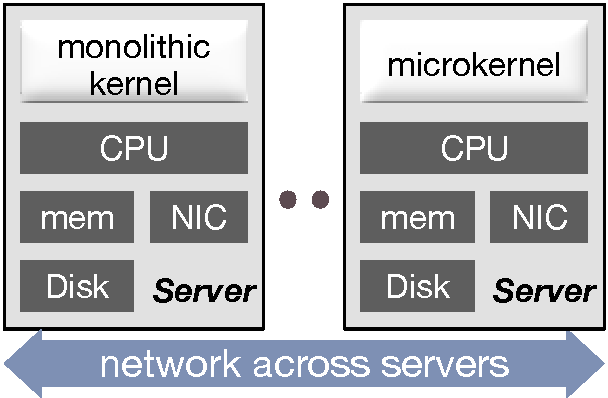
\includegraphics[width=1.7in]{lego/Figures/monolithic-arch.pdf}}
\caption[Monolithic OS.]{OSes Designed for Monolithic Servers.}
\label{fig-monolithic}
\end{center}
\end{subfigure}
\begin{minipage}{0.05in}
\hspace{0.05in}
\end{minipage}
\begin{subfigure}{1.8in}
\begin{center}
\centerline{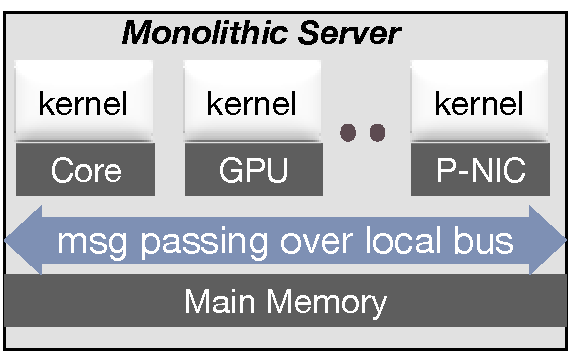
\includegraphics[width=1.8in]{lego/Figures/multikernel-arch.pdf}}
\caption[Multikernel Architecture.]{Multi-kernel Architecture. \small{P-NIC: programmable NIC.}}
\label{fig-multikernel}
\end{center}
\end{subfigure}
\begin{minipage}{0.05in}
\hspace{0.05in}
\end{minipage}
\begin{subfigure}{2.5in}
\begin{center}
\centerline{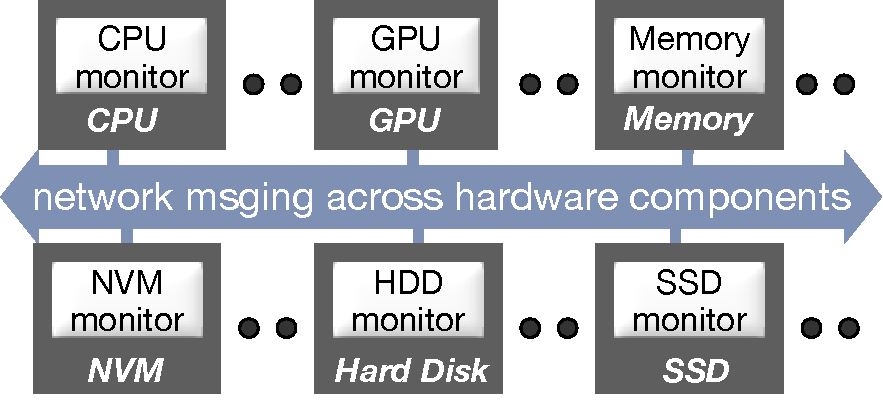
\includegraphics[width=2.6in]{lego/Figures/lego-arch.pdf}}
\caption[Splitkernel Architecture.]{Splitkernel Architecture.}
\label{fig-splitkernel}
\end{center}
\end{subfigure}
\caption[Operating System Architecture.]{Operating System Architecture.}
\end{figure*}
}

\ulinebfpara{Thread synchronization and data coherence.}
Threads and processes can share data even when they are not on the same \CN.
Similar to traditional concurrent programming, \sys\ threads can use synchronization primitives to build critical sections (\eg, with \syslock) 
and other semantics (\eg, flushing all requests with \fence).

An application can choose to cache data read from \sysread\ at the \CN\ (\eg, by maintaining \texttt{local\_rbuf} in the code example).
Different processes sharing data in a \rspace\ can have their own cached copies at different \CN{}s.
Similar to ~\cite{Shan18-OSDI}, \sys\ does not make these cached copies coherent automatically and lets applications choose their own coherence
protocols.
%mechanisms and policies.
%Note that maintaining coherence when caching shared data is not handled by DVMA automatically. 
We made this deliberate decision because automatic cache coherence on every read/write would incur  high performance overhead with commodity Ethernet infrastructure
and application semantics could reduce this overhead.
%(\eg, by infrequent messaging).
%to let users decide on their coherence mechanism on top of \sys\ and to prevent the potential high network communication overhead.
%if threads cache shared data, there can be multiple locations of caches. 
%We do not make these caches coherent automatically, as it could cause high network communication overhead.
%Users can manage coherence on their own.
%Different users can share memory and can use \sys's synchronization primitives to achieve inter-user synchronization (\eg, using \tas\ to define critical section). 


\subsection{\sys\ Architecture}

In \sys\ (Figure~\ref{fig-arch}), \CN{}s are regular servers each equipped with a regular Ethernet NIC and connected to a top-of-rack (ToR) switch.
\MN{}s are our customized devices directly connected to a ToR switch.
%
Applications run at \CN{}s on top of our user-space library called {\em \syslib}.
%\syslib\ handles application requests in the user space.
It is in charge of request ordering, request retry, congestion, and incast control. 
%\syslib\ issues raw Ethernet requests directly to the NIC (bypassing kernel with zero memory copy, similar to DPDK~\cite{DPDK}). 
%Similar to DPDK~\cite{DPDK}, \syslib\ bypasses kernel and has zero memory copy capability.

By design, an \MN\ in \sys\ is a \sysboard\ consisting of an ASIC which runs the hardware logic for all data accesses (we call it the {\em fast path} and prototyped it with FPGA),
an ARM processor which runs software for handling metadata and control operations (\ie, the {\em slow path}),
and an FPGA which hosts application computation offloading (\ie, the {\em extend path}).
An incoming request arrives at the ASIC and travels through standard Ethernet physical and MAC layers 
and a Match-and-Action-Table (MAT) that decides which of the three paths the request should go to based on the request type.
If the request is a data access (fast path), it stays in the ASIC and goes through a hardware-based virtual memory system
that performs three tasks in the same pipeline: address translation, permission checking, and page fault handling (if any).
Afterward, the actual memory access is performed through the memory controller, and the response is formed and sent out through the network stack.
Metadata operations such as memory allocation are sent to the slow path. % and handled in software that runs on Linux at the ARM processor.
Finally, customized requests with %customized, high-level operations such as pointer chasing and 
offloaded computation are handled in the extend path.
%which executes the corresponding application offload.
%The offload itself could internally issue data and metadata operations to the fast and the slow paths.
%In the rest of the paper, we focus on the design of the fast and the slow paths and how they interact with each other.






\if 0
\subsection{Paper Scope And Potential Extensions}
\label{sec:scope}
%We made it real by building an open-source, distributed smart hardware-based disaggregated memory framework.
This paper focuses on the low-level systems problem of how to most efficiently build an \MN\ hardware device and to support it with \CN-side software. 
In real deployment, a single \sysboard\ is usually insufficient.
A distributed set of \sysboard\ would allow applications to allocate and access memory from multiple \MN{}s using a unified virtual memory interface. 
Systems like LegoOS~\cite{Shan18-OSDI} and Clover~\cite{Tsai20-ATC} have demonstrated how to build a distributed \MN\ platform.
For example, LegoOS uses a “two-level” approach, where a global controller manages the entire memory space at coarse granularity and each \MN\ manages its own memory at fine granularity (like how \sysboard\ does). Each \MN\ can be over-committed (\ie, allocating more virtual memory than its physical memory size), and when an \MN\ is under memory pressure, it migrates data to another \MN\ (coordinated by the global controller).
In addition, LegoOS leaves the handling of \MN\ failure to applications, since most data-center applications already have their own reliability mechanisms.
A similar mechanism could be used to extend \sys\ to a distributed system, and we leave it for future work.

Another potential extension to our current implementation of \sys\ is a transparent user interface.
By design, \sys’s APIs can be called by different layers: directly by applications as what we show in this paper, by a runtime like the AIFM runtime~\cite{AIFM}, or by the kernel/hardware at \CN\ like LegoOS' pComponent~\cite{Shan18-OSDI}. \sysboard\ doesn’t need any change to support any of these usages.
The latter two usages of \sysboard\ would result in a transparent interface and allow the use of unmodified user applications.
For example, for the last case, the \CN\ kernel or hardware captures misses in \CN’s local memory and then calls \sys’s APIs to fulfill the misses.
%(after porting \syslib\ to the kernel space or to hardware).

\fi


%\yizhou{Clio architecture shares a lot similarities with disaggregated storage systems such as fiber channel storage area network (FC SAN). The key difference is that Clio targets microsecond-level disaggregated memory system which poses stricter requirements on the system design.}


%\yizhou{
%1) I think we should explicitly say "By design, MN consists of ASIC, FPGA, and ARM parts.. In our impl, the ASIC part is using FPGA too." I get the motive behind it. The way it is described makes readers think this is the real stuff. 2) Similarly, the customized extend path does not really have to be FPGA as well. It could be ASIC too. In all, I suggest differentiate "by design" and "our impl".}

\if 0

\section{Hardware-Based Virtual Disaggregated Memory}
\label{sec:vdm}

We advocate for a new approach for memory disaggregation:
a hardware-based ``smart'' virtual disaggregated memory system.
Specifically, this approach encorporates the following design principles.
%We believe that disaggregated memory should be managed at the memory side behind a per-client virtual memory abstraction, 
%but without the reliance on a host server and with the support for computation offloading.
%With a per-client virtual memory abstraction, 
%application-level programs and low-level systems like databases and JVM can all sit on \sys\ with each of them properly isolated,
%and the physical location of disaggregated memory can be transparent and thus non-contiguous and moved around.
%By building a hardware-based ``smart'' virtual disaggregated memory system,
%we can achieve low-latency performance, scalability, efficient memory utilization, low cost, and ease of management,
%as what the rest of this paper will show.
%Below are the principles that guide the design of \sys.

\boldpara{Managing memory at \MN{}s and exposing a per-client virtual memory abstraction.}
We manage disaggregated memory entirely within a disaggregated memory pool by building a virtual memory system at each \MN.
By encapsulating management in the disaggregated memory pool and allowing client applications to
access it as a black box,
we can achieve independent, transparent resource pool management,
which is a key reason behind industry's wide adoption of storage disaggregation~\cite{FACEBOOK-BRYCECANYON,FB1,SnowFlake-NSDI20,Ali-SinglesDay}. %why storage disaggregation has become the recent industry norm;
It also avoids the network communication overhead incurred in solutions that handle some or all management tasks at \CN{}s.

We choose to expose a {\em per-client virtual memory} abstraction,
where each client has an isolated space that it can access with virtual memory addresses at byte granularity.
%\textbf{Q1)} \textit{what abstraction disaggregated memory exposes}?
%Disaggregated memory should expose an abstraction that is versatile enough to support many different uses.
%One such abstraction is {\em per-client virtual memory},
Just like the classical virtual memory abstraction, this abstraction is low-level and generic enough to support many applications
and high-level enough to protect and hide raw memory. 
%This abstraction inherits the versatility and transparency benefits of the classical virtual memory abstraction. %process address spaces:
%1) application-level programs and low-level systems like databases and JVM can all sit on the same abstraction
%with each of them properly isolated,
%and 2) the physical location of disaggregated memory can be transparent and thus non-contiguous and moved around.
%The abstraction we believe to be the best fit for memory disaggregation is a virtual memory interface that is facing client processes running at \CN{}s.
%With this abstraction, disaggregated memory can be managed at \MN{}s, which is more efficient and flexible than at \CN{}s (\S\ref{sec:intro} and \S\ref{sec:pdm}).
%It is worth noticing that %\sys\ is a versatile system that can either 
For example, memory disaggregation solutions that operate below the application level,
\eg, language runtime~\cite{Semeru}, data-structure library~\cite{AIFM}, swap system~\cite{InfiniSwap,FastSwap}, %\fixme{anything else?},
can sit on top of \sys. % and are orthogonal to our work. 
They can be ported to \sys\ by replacing their RDMA-/messaging-based abstraction to \sys's virtual memory abstraction. % (Figure~\ref{fig-usage} U3).

\boldpara{Building a virtual memory system in hardware.}
We demonstrate that \MN{}s can be built as standalone hardware devices without a server box,
as its benefits outweigh the complexity of hardware development.
Building \MN\ as a single hardware device avoids the monetary cost of a whole server box and the energy cost of a power-hungry CPU.
It also avoids the performance overhead of NIC talking to the host server for handling virtual memory tasks like page fault handling.
Moreover, a hardware implementation could allow greater parallelism and customized pipelines
that is crucial in supporting disaggregate memory's scalability goals (TB-level memory, thousands of clients)
and in meeting today's and future high-speed network line rate~\cite{TONIC}.
%Today's disaggregated memory systems unfortunately have a strong reliance on host CPU, MMU, and OS
%for running a virtual memory system, even though these systems themselves do not necessarily need to run anything at the host server.
%The solution is obvious but never carried out before: building the virtual memory system in \MN\ hardware.

\boldpara{Designing a network layer that exploits memory disaggregation's unique features.}
We improve network communication performance and reduce its costs by 
exploiting the unique nature of memory disaggregation. % to co-design a new network layer.
%Unfortunately, existing disaggregated memory systems lose this optimization opportunity by sitting on RDMA or TCP.
Unlike general-purpose network solutions such as TCP and RDMA that have the same design for all endpoints (\ie, symmetric),
the network system for disaggregated memory can be {\em asymmetric}, as \CN{}s are always the request initiator and \MN{}s only respond to requests.
%RDMA and TCP have two fundamental features that make them unfit for memory disaggregation:
%1) they have the same design for all endpoints (\ie, symmetric),
%while memory disaggregation are asymmetric in nature (\CN{}s are always the request initiator and \MN{}s only respond to requests);
Moreover, not all memory operations require strict ordering.
Thus, we can relax network layer's reliability guarantees (\eg, allowing packet reordering)
and enforce (weaker) orderings at the memory operation level.
%2) their reliable transports are connection-based and follow strict packet ordering.
%These features result in scalability bottlenecks and added hardware complexity.
%However, as we will show in \S\ref{sec:network}, neither are required if we can customize the network layer for the client-facing virtual memory model.

\boldpara{Supporting computation offloading with a unified virtual memory view.}
The network communication between \CN{}s and \MN{}s is the major cause of disaggregated memory's performance overhead.
To reduce this overhead, applications should be able to offload their less computation-intensive tasks to \MN{}s.
\sys\ offers a unified virtual memory view for application computation at both \CN\ and \MN.
%and offloads running at \MN{}s cannot have a coherent memory view with computation running at \CN{}s.
Furthermore, running offloaded computation in hardware is a desired option, %reduces \MN{}'s energy cost 
as it could achieve more parallelism and performance customization while avoiding CPU energy cost.
\sys\ allows offloads that run in hardware to use the \sys\ virtual memory interface in the same way as how software runs on \sys.
%However, %a major obstacle of hardware-based offloading currently is 
%it is hard to offload computation to \MN\ hardware today,
%largely because there is no good system support for offloads to use (virtualized) memory
%We build an offloading framework that offers a unified virtual memory view for application computation at both \%CN\ and \MN.
%applications should be able to easily and safely offload their less computation-intensive tasks to \MN{}s.




\section{Hardware Active Disaggregated Memory}
\label{sec:phdm}

%This section gives an overview of the \phdm\ model, 
%its benefits, and its use cases.

%\subsection{\phdm\ Overview}
%\label{sec:phdmoverview}

\phdm\ has a server-based compute pool that runs applications
and a separate memory pool that consists of network-attached hardware memory devices.
%\phdm\ has a distributed, network-attached memory pool 
%that is separated from the compute pool.
%\phdm\ manages memory at the remote memory pool.
%and runs applications at the compute pool.
An application process running at a \CN{} can use memory from any \MN{},
and an \MN{} can host data for many applications running on different \CN{}s.
%With this design of disaggregated and distributed memory services,
Thus, \phdm\ delivers independent management and scaling of memory and compute pools 
and efficient memory resource utilization.
%Doing so reduces network RTTs and makes management tasks such as configuration, upgrade, and failure handling easy
%with no or little disturbance to \CN{}s.

An \phdm\ system manages and virtualizes physical memory at \MN{}s
and offers one or more {\em distributed memory services}.
\phdm\ provides a protected, client-centric virtual memory abstraction 
and potentially more higher-level memory service interfaces.
Applications running at \CN{}s can directly and safely use these interfaces to access remote memory. % and be protected from each other.
%These services have a client-centric view, providing interfaces that can directly and easily be used by clients 
%and offering proper protection across different applications.
%It provides high-level memory services and
% can support new types of applications that require large memory space, 
%inter-node memory sharing, or fast data storage.
%Section~\ref{sec:usecases} gives several examples of \phdm\ memory services.

\phdm\ executes all performance-critical tasks on hardware at \MN{}s,
%As explained in \S\ref{sec:disaggregation}, 
%With fast increasing datacenter network bandwidth, \MN{}s need to be able to serve large amounts of 
%requests concurrently to deliver {\em network line-rate} performance.
%Running software in many-core CPU could potentially meet the performance requirement but comes with high monetary and energy cost,
%while running software in low-energy ``wimpy'' cores cannot keep up with high network line rate.
%as handling memory requests in hardware is critical in meeting 
as doing so can meet the performance, scalability, and cost goals of remote memory systems.
With varying application needs in today's datacenters,
disaggregated memory systems should be flexible enough to provide different services and interfaces.
Thus, in our proposed \phdm\ model, the remote memory layer is {\em reconfigurable}.
%We further propose to implement \phdm's memory services on programmable hardware
%to meet our target usage and deployment models:
Specifically, an \MN{} can be configured to offer different (sets of) memory services,
but once a cluster of \MN{}s are configured they are only reconfigured when 
there is a need to change, patch, or upgrade services.
This model is in line with Microsoft's FPGA deployment~\cite{Catapult}
and what we view as a good use of reconfigurable hardware in datacenters.

\if 0
Finally, we view \phdm\ as a general model that can have different hardware choices for \MN{}s,
as long as they incorporate some programmable hardware for performance-critical and non-fixed tasks in memory services
(\eg, a single FPGA, FPGA+SoC, ASIC+FPGA, or ASIC+FPGA+SoC).
Non-performance-critical tasks can run in software, and fixed functionalities can run in non-programmable hardware.
\fi


%\subsection{Use Cases}
%\label{sec:usecases}
Many types of applications can make use of \phdm.
%In some cases, applications could explicitly call APIs an \phdm\ service provides
%(and be aware of the disaggregated nature of their in-memory data).
%In other cases, they could transparently access an \phdm\ service without knowing the disaggregated or remote nature.
Below we give some examples. % on what services an \phdm\ system can provide and how applications can use them.
We implemented an instance of the first three types in this paper,
leaving the rest for future work.

\boldpara{Extended (semantic-rich) virtual memory.}
A basic service \phdm\ can provide is a remote virtual memory space that lets applications
store in-memory data (\eg, as extended, slower heaps).
%Similar to traditional process address spaces, each application process on each \CN{}
%can have their own remote address space that \phdm\ protects from other processes'.
In addition to simple, hardware-like virtual memory APIs such as reading and writing to a memory address, 
\phdm\ could provide higher-level APIs like synchronization primitives, pointer manipulation, 
vector and scatter-gather operations~\cite{Aguilera-FarMemory}.
Applications and language libraries can then build complex data structures like vectors 
and trees with these APIs.
%We implemented this extended virtual memory service in \sys.

\boldpara{In-memory and ephemeral storage.}
\phdm\ could offer in-memory storage services such as distributed key-value stores, databases, and file systems.
With \phdm, many storage operations (\eg, key-value pair lookup, SQL select) 
could be implemented in hardware at where the data is, offering enhanced performance. 
%In addition, built-in distributed support in \phdm\ could be used to offer high availability and failure resilience
%to the in-memory storage services.
\phdm\ is also a good fit for building ephemeral storage and storage caching that do not require failure resilience~\cite{SnowFlake-NSDI20,Pocket,fitzpatrick2004distributed}.
%We implemented a distributed key-value store in \sys\ with optional replication support.

\boldpara{Data sharing.}
Since multiple \CN{}s can access the same \MN{}s in \phdm,
\phdm\ could be used for data sharing and communication across \CN{}s.
This is especially useful for new datacenter services like serverless computing~\cite{Berkeley-Serverless},
which currently has no or poor support for managing states and inter-function communication.
With \phdm, serverless functions can run on \CN{}s and store states or communication messages in the disaggregated memory layer.
Similarly, \phdm\ can also be used for storing global states such as the parameter server in distributed machine learning systems.
%We implemented a multi-version data sharing service in \sys\
%that can be accessed by different \CN{}s concurrently.

\boldpara{Offloading data processing.}
\phdm\ is a good candidate for offloading data processing and data analytics. 
Data-intensive applications can offload computation that frequently access in-memory data together with 
these data to \MN{}s.
One such example is disaggregated Spark shuffle~\cite{Stuedi-ATC19}, where the shuffle
operation could be implemented in programmable hardware and the shuffle data could be 
stored in \MN{}s of \phdm.

\boldpara{Remote swap and remote disk.}
Legacy applications and libraries can also benefit from \phdm\ in a transparent way.
Two such examples are remote memory-based disk and remote swap~\cite{InfiniSwap}.
The OS at the \CN{}s can add a memory-based block device that sits in \phdm\
in a similar way as building the {\em ramdisk} module.
Applications can directly use this new device or use it as a swap space.

\boldpara{Disaggregated OS.}
Recently, there have been proposals to completely disaggregate memory from compute.
\lego~\cite{Shan18-OSDI} is such a proposal that organizes compute nodes as processors with no memory 
and \MN{}s as memory devices with no computation.
%While \lego\ currently only works on emulated hardware, it can build on \phdm\ to have a 
%real hardware solution.
\lego\ can build on \phdm\ by configuring \CN{}s as its compute nodes %(called {\em pComponent}s) 
and \MN{}s as its memory nodes. %(called {\em mComponent}s).


\fi

\section{SuperNIC Board Design}
\label{sec:snic:design}

{
\begin{figure*}[th]
\begin{center}
\centerline{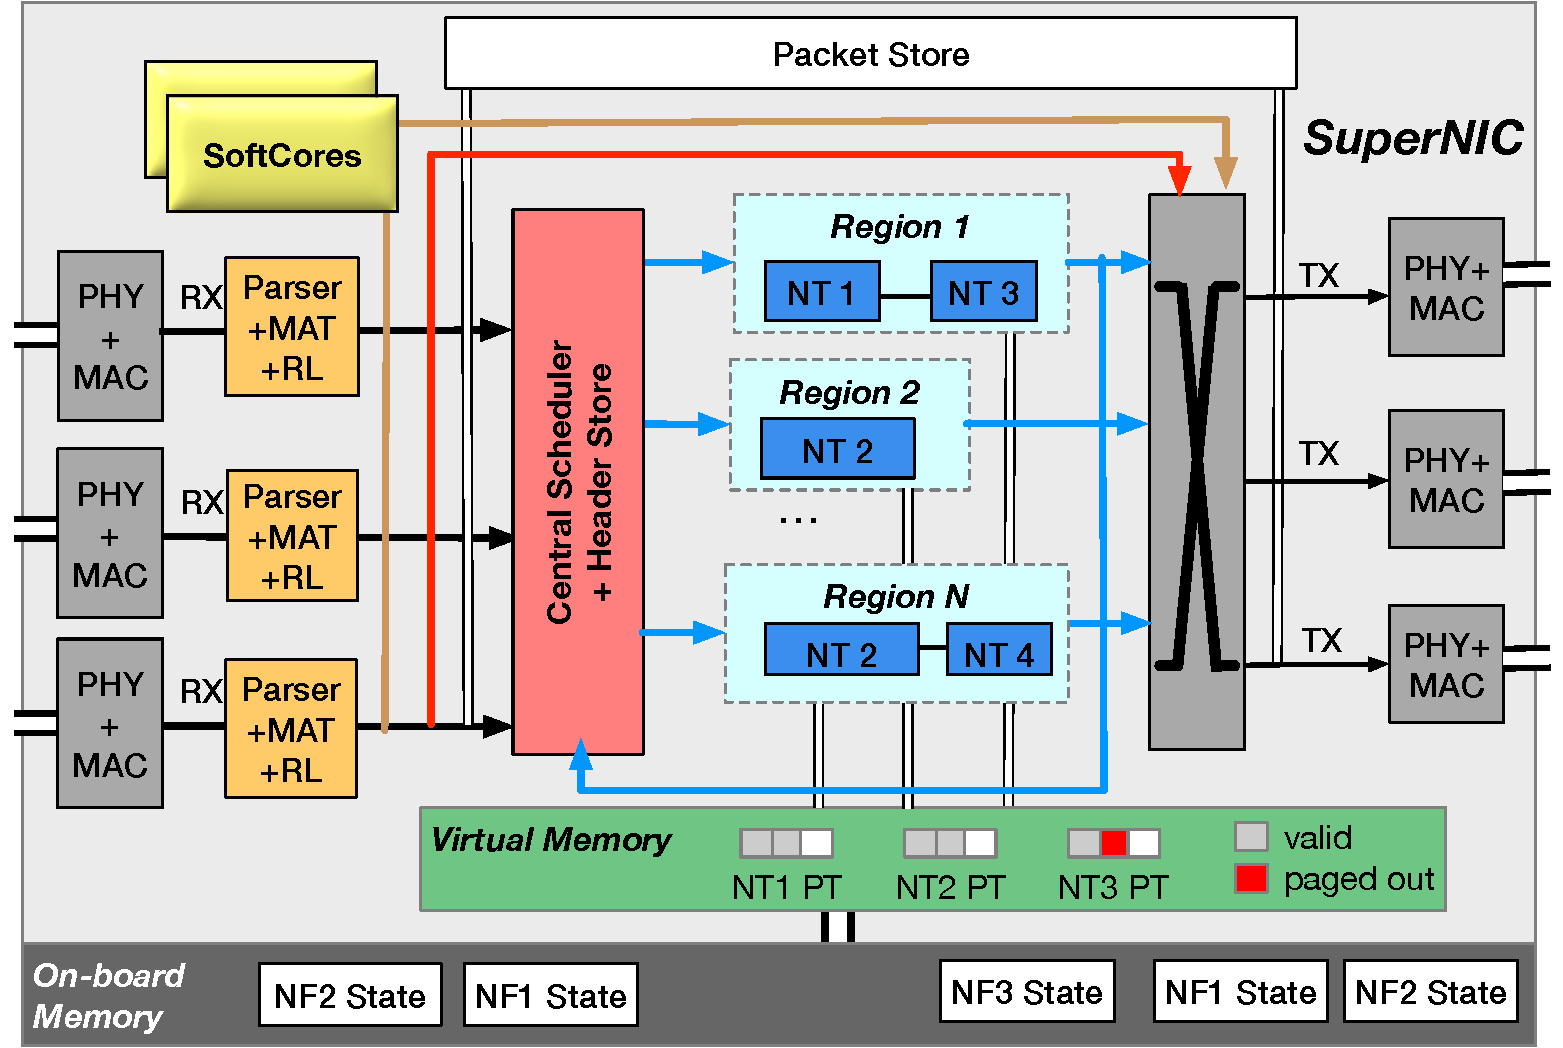
\includegraphics[width=\textwidth]{snic/Figures/board.pdf}}
\mycaption{fig-snic-board}{\snic\ On-Board Design.}
{
RL: Rate Limiter. PT: Page Table
}
\end{center}
\end{figure*}
}
{
\begin{figure*}[th]
\begin{center}
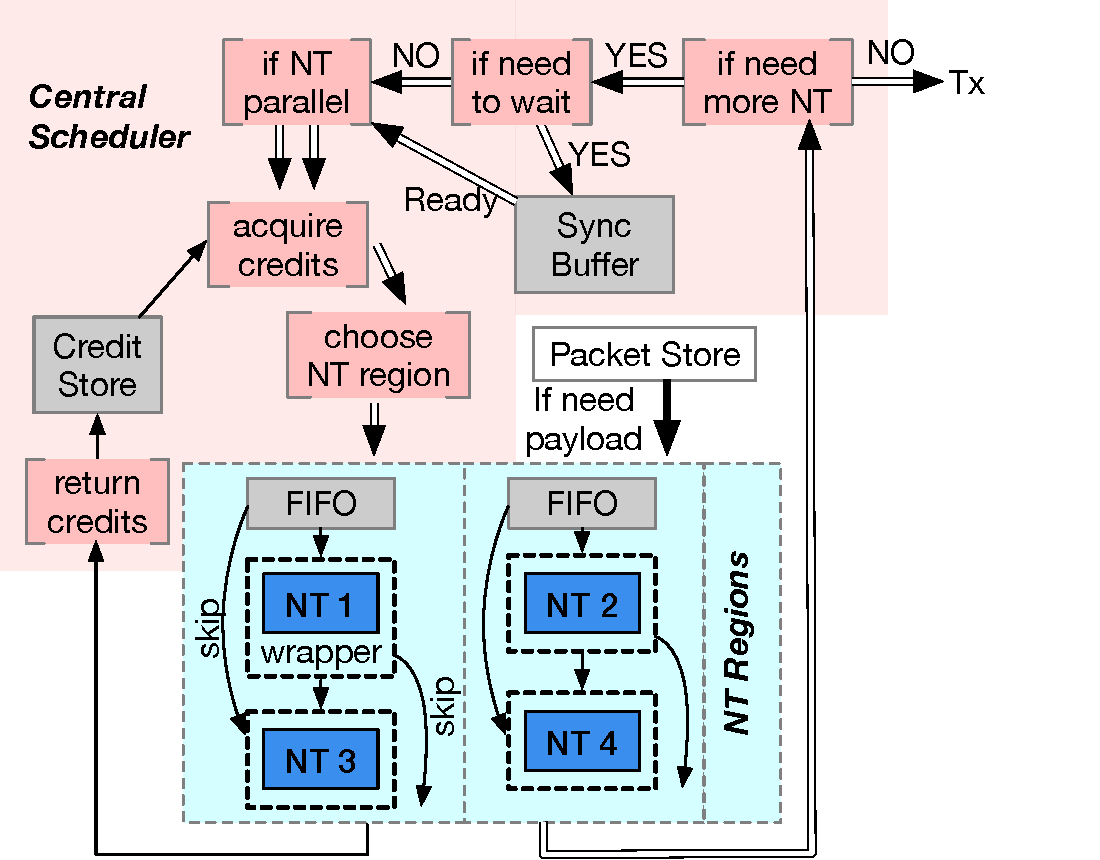
\includegraphics[width=0.9\textwidth]{snic/Figures/scheduler.pdf}
\mycaption{fig-sched}{\snic\ Packet Scheduler and \nt\ Region Design.}
{
Double arrows, single arrows, and thick arrows represent packet headers, credits, and packet payload.
}
\end{center}
\end{figure*}
}

Traditional server SmartNICs have plenty of hardware resources when hosting network functions for applications running on the local server~\cite{SmartNIC-nsdi18,Caulfield-2018}.
In contrast, \snic{} is anticipated to often be fully occupied or even over-committed, as it needs to host \nt{}s from more tenants with limited hardware resources to save costs.
Thus, a key and unique challenge in designing \snic{}s is space- and performance-efficient consolidation in a multi-tenant environment.
Moreover, \snic\ faces a more dynamic environment where not only the load of an application but also applications themselves could change from time to time.
Thus, unlike traditional SmartNICs that focus on packet processing and packet scheduling, \snic\ also needs to schedule \nt{}s efficiently.
%, and both types of scheduling needs to accommodate to a dynamic, multi-tenant environment.
%be more scalable and more flexible.
This section first goes over the high-level architecture of \snic, then discusses our mechanisms for efficient packet and \nt\ scheduling, followed by the discussion of our scheduling and fairness policies, and ends with a description of \snic's virtual memory system.
%We handle the former with SoftCores and the latter with hardware.
%An \snic\ has three major tasks: packet processing, packet scheduling, and \nt\ scheduling.
%overall approach \fixme{TODO if have space}  

\subsection{Board Architecture and Packet Flow}

We design the \snic\ board to simultaneously achieve several critical goals:
\textbf{G1)} parsing/de-parsing and scheduling packets at line rate;
\textbf{G2)} high-throughput, low-latency execution of \nt\ DAGs;
\textbf{G3)} safe and fair sharing of all on-board resources;
\textbf{G4)} quick adaptation to traffic load and workload changes;
\textbf{G5)} good scalability to handle many concurrent workloads and \nt{}s;
\textbf{G6)} flexible configuration and adjustment of control-plane policies;
and \textbf{G7)} efficient usage of on-board hardware resources.
%using most of the on-board hardware resources for application \nt{}s.
Figure~\ref{fig-snic-board} illustrates the high-level architecture of the \snic\ board.

\snic's data plane consists of reconfigurable hardware (\eg, FPGA) for running user \nt{}s (blue parts in Figure~\ref{fig-snic-board})
and a small amount of non-reconfigurable hardware (ASIC) for non-user functionalities, similar to the ``shell'' or ``OS'' concept~\cite{Catapult-v2,Amazon-F1,amorphos-osdi18,coyote-osdi20}.
We choose a hardware-based data-plane design because \nt{}s like transports demand high-speed, parallel processing, and a fully reconfigurable hardware allows the maximum flexibility in \nt\ hardware designs.
Many of our design ideas can potentially be applied to other types of hardware and software \nt\ implementations, such as PISA pipelines and ARM cores.
%In our prototype, 90\% space of the \snic\ chip is dedicated for \nt{}s (\textbf{G7}).

We divide the \nt\ area into {\em region}s, each of which could be individually reprogrammed to run different \nt{}s.
Different \nt\ regions can be executed in parallel.

The control plane runs as software on a small set of general-purpose cores (SoftCores for short) (\eg, a small ARM-based SoC). 
To achieve the performance that the data plane requires and the flexibility that the control plane needs, we cleanly separate these two planes.
The data plane handles all packet processing on ASIC and FPGA (\textbf{G1}).
The control plane is responsible for setting up policies and scheduling \nt{}s and is handled by the SoftCores (\textbf{G6}).
In our prototype, we built everything on FPGA. 


When a packet arrives at an RX port, it goes through a standard physical and reliable link layer.
Then our parser parses the packet's header and uses a Match-and-Action Table (MAT) to decide where to route the packet next.
The parser also performs rate limiting for multi-tenancy fairness (\S\ref{sec:snic:policy}).
The parser creates a packet descriptor for each packet and attaches it to its header. The descriptor contains fields for storing metadata, such as an \nt\ DAG UID and the address of the payload in the packet store. 
The SoftCores determine and install rules in the MAT, which include three cases for routing packets to the next step.
%There are three cases.
First, if a packet specifies no \nt\ information or is supposed to be handled by another \snic\ (\S\ref{sec:snic:dist}), the \snic\ will only perform simple switching functionality and send it to the corresponding TX port (red line).
Second, if a packet specifies the operation type \texttt{CTRL}, it will be routed to the SoftCores (orange line). These packets are for control tasks like adding or removing \nt{}s, adding \nt\ DAGs (\S\ref{sec:snic:ntsched}), and control messages sent from other \snic{}s (\S\ref{sec:snic:dist}).

Finally, all the remaining packets need to be processed on the \snic, which is the common case.
Their payloads are sent to the {\em packet store}, and their headers go to a central scheduler (black arrows). 
The scheduler determines when and which \nt\ chain(s) will serve a packet and sends the packet to the corresponding region(s) for execution (blue arrows).
If an \nt\ needs the payload for processing, the payload is fetched from the packet store and sent to the \nt.
During the execution, an \nt\ could access the on-board memory through a virtual memory interface, in addition to accessing on-chip memory.
After an \nt\ chain finishes, if there are more \nt{}s to be executed, the packet is sent back to the scheduler to begin another round of scheduling and execution.
When all \nt{}s are done, the packet is sent to the corresponding TX port.
%, which uses an arbiter to guarantee bandwidth fairness across applications.


\subsection{Packet Scheduling Mechanism}
\label{sec:snic:packetsched}

We now discuss the design of \snic's packet scheduling mechanism. Figure~\ref{fig-sched} illustrates the overall flow of \snic's packet scheduling and execution.
%To efficiently execute such complex \nt\ DAGs, we first propose the concept of {\em \nt\ chain}, which allows one packet to be processed by a chain of \nt{}s without the need to go through the scheduler multiple times.
%Second, we build a flexible run-time system that supports both {\em \nt-level parallelism} (running different \nt{}s in parallel) and {\em instance-level parallelism} (running multiple instances of the same \nt{}s in parallel) in hardware.
%Existing hardware-based network function systems like Click~\cite{clicknp-sigcomm16}, E2~\cite{e2-sosp15}, and PANIC~\cite{panic-osdi20} focus on scheduling a single NF or a simple sequence of NFs with instance-level parallelism.
%\snic\ provides all three types of scheduling: \nt\ chaining, \nt-level parallelism, and instance-level parallelism, and in a scalable, efficient way.
%Doing so achieves high-throughput, low-latency \nt\ DAG execution (\textbf{G2}), quick adaptation to traffic load changes (\textbf{G4}), and fast and scalable scheduling (\textbf{G5}).

\bolditpara{\nt-chain-based FPGA architecture and scheduling.}
%Today's network systems are seeing increasing amounts of network functions that can be executed as a DAG (\eg, previous work found 53.8\% NF pairs can run in parallel~\cite{NFP-sigcomm17}).
As \snic\ enables more types of endpoints and workloads to offload their network tasks, the number of \nt{}s and their execution flows will become even more complex, which could impact both the complexity of board design and the performance of packet scheduling.
Our idea to confront these challenges is to execute as many \nt{}s as possible in one go, by chaining \nt{}s together.
%There can be different ways to split an \nt\ DAG can 
We put chained \nt{}s (called an {\em \nt\ chain}) in one \nt\ region (\eg, \nt{}1$\xrightarrow[]{}$\nt{}3 and \nt{}2$\xrightarrow[]{}$\nt{}4 in Figure~\ref{fig-snic-board}).
%A packet that uses a chain goes through all the \nt{}s in the chain without the need to involve the scheduler in between.
Instead of connecting each \nt\ to a central scheduler (as what PANIC~\cite{panic-osdi20} does), we connect each region to the scheduler.
Doing so allows us to use a much smaller crossbar between the \nt\ regions and the central scheduler, thereby reducing hardware complexity and area cost (\textbf{G7}).

Furthermore, we leverage \nt\ chains to reduce the scheduling overhead and improve the scalability of the central scheduler.
Our idea is to {\em reserve} credits for an {\em entire} \nt\ chain as much as possible and then execute the chain as a whole; only when that is not possible, we fall back to a mechanism that may involve the scheduler in the middle of a chain. 
Doing so reduces the need for a packet to go through the scheduler after every \nt, thereby improving both the packet's processing latency and the central scheduler's scalability (\textbf{G5}).

On top of the fixed chain design, we propose an optimization to enable efficient \nt\ time sharing across multiple users and to accommodate cases where some packets of an application only access a part of a chain (\textbf{G4}, \textbf{G6}).
Our idea is to support the {\em skipping} of arbitrary \nt(s) in a chain.
For example, a user can access \nt{}1 and \nt{}4 by first skipping \nt{}3 in Region-1 and then skipping \nt{}2 in Region-2 in Figure~\ref{fig-sched}.


\noindent{\ul{\textbf{Scheduling packets with \nt-level and instance-level parallelism.}}}~~
At an \snic, different regions run in parallel.
We exploit two types of parallelism by controlling what \nt{}s to put in parallel regions.
The first type concurrently executes {\em different packets} at multiple instances of the {\em same \nt\ chain} (what we call {\em instance-level parallelism}).
We automatically create more/less instances of an \nt\ chain based on load and send different packets in a round-robin way to the parallel instances.
We will discuss our \nt\ autoscaling policy in \ref{sec:snic:policy}.


The second type concurrently executes the {\em same packet} at multiple {\em different \nt{}s} (what we call {\em \nt-level parallelism}).
We infer what \nt{}s can run in parallel in an \nt\ DAG (\eg, in Figure~\ref{fig-nt-example}, \nt{}1 and \nt{}2 can run in parallel with \nt{}3 for user1).
We expect a fair amount of opportunities to explore \nt-level parallelism, as previous work found that 53.8\% NF pairs can run in parallel~\cite{NFP-sigcomm17}.
To execute a packet at several \nt{}s concurrently, the scheduler makes copies of the packet header and sends them to these \nt{}s concurrently. To obey the order of \nt{}s that users specify, we maintain a {\em synchronization buffer} to store packet headers after they return from an \nt{}'s execution and before they could go to the next stage of \nt{}s (Figure~\ref{fig-sched}).

{
\begin{figure*}
\begin{center}
\centerline{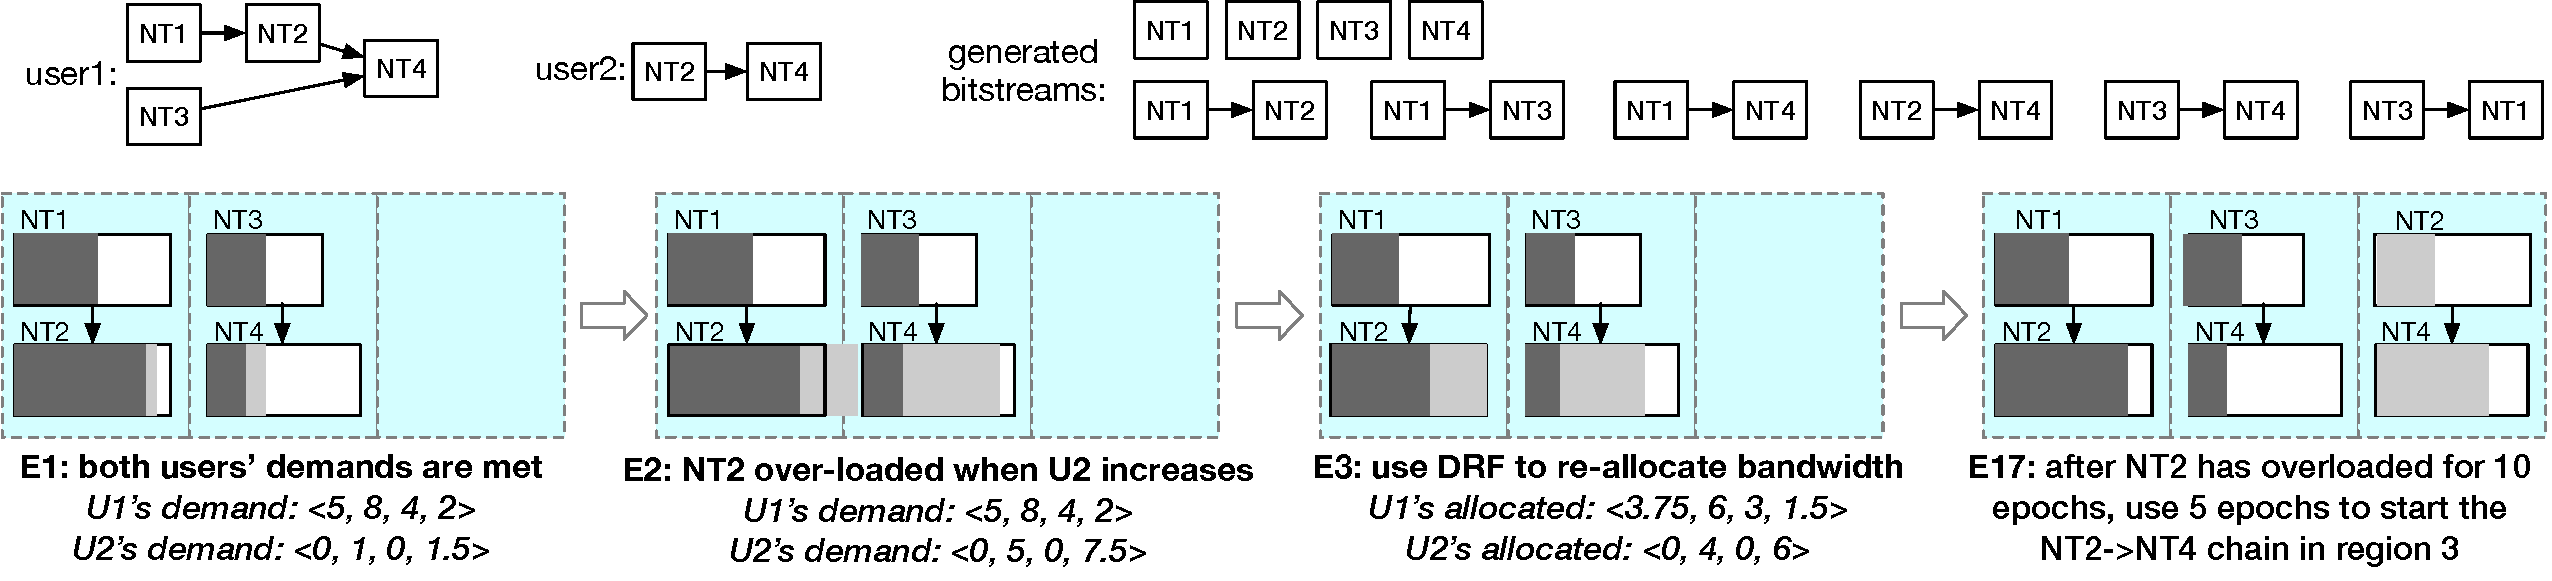
\includegraphics[width=0.9\textwidth]{Figures/nt-example.pdf}}
\vspace{-0.1in}
\mycaption{fig-nt-example}{An Example of \nt\ chaining and scheduling.}
{
Top: user1 and user2's \nt\ DAGs and \snic's generated bitstreams for them.
Bottom: timeline of \nt\ bandwidth allocation change.
Dark grey and light grey represent user1 and user2's load.
The launched chains are \nt{}1$\xrightarrow[]{}$\nt{}2 and \nt{}3$\xrightarrow[]{}$\nt{}4,
with \nt{}2 and \nt{}4 being shared by the two users.
The maximum throughput of NT1, NT2, and NT4 are 10 units each, and NT3's is 7 units.
NT2 is the dominant resource for user1, and NT4 is the dominant for user2.
}
\end{center}
\vspace{-0.2in}
\end{figure*}
}


\subsection{\nt\ (De-)Launching Mechanism}
\label{sec:snic:ntsched}
\snic's SoftCore handles \nt\ deployment, launch, and scheduling tasks, as a part of the control path.
A new challenge specific to \snic\ comes from the need to do more frequent \nt\ reconfigurations than traditional programmable network devices.
To enable more consolidation, we allow multiple \nt{}s to {\em time share} an FPGA space, and we auto-scale \nt{}s.
Both these cases involve the slow FPGA PR process.
We propose a set of new mechanisms and policies to reduce or hide the PR costs.
We now discuss the mechanisms and defer the policy discussions to \S\ref{sec:snic:policy}.

\bolditpara{\nt\ deployment.}~~
Users deploy \nt{}s to the \snic\ platform ahead of time as FPGA netlists (which can be thought of as Intermediate Representations in software).
When receiving newly deployed \nt{} netlists for an application, we first generate a set of FPGA bitstreams (which can be thought of as executable binaries in software).
We enumerate all possible combinations of \nt{}s under user-specified \nt\ DAG ordering requirements when generating bitstreams. 
This is because bitstream generation is a slow process that usually takes a few hours or even longer. 
Generating more bitstreams at deployment time gives the \snic\ more flexibility to choose different \nt\ combinations at the run time. 
Figure~\ref{fig-nt-example} shows an example of generated bitstreams based on two DAGs of two users.
%\noteyiying{delete the following sentence if need more space}
%We do not generate bitstreams for three-\nt{} chains in this example, as that exceeds what a region can hold.
%For example, with three \nt{}s where the user specifies the first two to fan in to the third, we generate bitstreams for \nt{}1, \nt{}2, \nt{}3, \nt{}1$\xrightarrow{}$\nt{}2, \nt{}2$\xrightarrow{}$\nt{}1, \nt{}1$\xrightarrow{}$\nt{}3, \nt{}2$\xrightarrow{}$\nt{}3, \nt{}1$\xrightarrow{}$\nt{}2$\xrightarrow{}$\nt{}3, and \nt{}2$\xrightarrow{}$\nt{}1$\xrightarrow{}$\nt{}3.
We store pre-generated bitstreams in the \snic{}'s on-board memory; each bitstream is small, normally less than 5\MB.

When generating bitstreams, we attach a small \snic\ wrapper to each \nt\ (Figure~\ref{fig-sched}).
%This module monitors the load of each \nt\ and \yiying{Will, what else is in the module?}
This wrapper is essential: it enables skipping an \nt\ in a chain (\S\ref{sec:snic:packetsched}), monitors the runtime load of the \nt\ (\S\ref{sec:snic:policy}), ensures signal integrity during PR, and provides a set of virtual interfaces for \nt{}s to access other board resources like on-board memory (\S\ref{sec:snic:memory}).

\bolditpara{\nt\ chain launching.}~~
We start a new \nt\ chain when an application is deployed (pre-launch), when the chain is first accessed by a packet in an application (on-demand), or when we scale out an existing \nt\ chain. For the first and third cases, we start the new \nt\ only when there is a free region (see \S\ref{sec:snic:policy} for detail).
%The SoftCore picks a free region to launch the chain. 
For the on-demand launching case, when all regions are full, we still need to launch the new chain to be able to serve the application. In this case, we need to de-schedule a current \nt\ chain to launch the new chain (see \S\ref{sec:snic:policy} for how we pick the region).

The \snic\ SoftCore handles this context switching with a {\em stop-and-launch} process.
Specifically, the SoftCore sends a signal to the current \nt{}s to let them ``stop''.
These \nt{}s then store their states in on-board memory to prepare for the stop.
At the same time, the SoftCore informs the scheduler to stop accepting new packets. 
The scheduler will buffer packets received after this point.
After the above {\em stop step}s finish, the SoftCore reads the new bitstream from the on-board memory via DMA and starts the FPGA PR process ({\em launch}).
This process is the slowest step, as the maximum reported achievable PR throughput is around 800\,MB/s~\cite{coyote-osdi20}, or about 5\,\ms\ for our default region size.
Afterwards, the newly launched chain can start serving packets, and it will first serve previously buffered packets, if any.

%\boldpara{Swap and victim region.}~~
%A unique and new challenge in scheduling \nt{}s in FPGA is that unlike software, the \nt\ region reconfiguration process as described above is slow. 
%We tackle this challenge from both the mechanism and policy perspectives.
%We now discuss our ideas in mechanisms.

To reduce the overhead caused by \nt\ reconfiguration, we use a technique similar to the traditional victim cache design. We keep a de-scheduled \nt\ chain in a region around for a while unless the region is needed to launch a new chain. If the de-scheduled \nt\ chain is accessed again during this time, we can directly use it in that region, reducing the need to do PR at that time.

%we always leave one or few regions empty; we call them {\em swap region}s.
%To start a new chain, the SoftCore directly launches it in one swap region and start processing new packets with it.
%In the background, the SoftCore de-schedule an \nt\ chain by performing the {\em stop} step as illustrated above to create one more swap region.
%This swap region approach allows us to reduce the reconfiguration time to only the {\em launch} time. 

%Our second idea is inspired by victim cache in the traditional CPU architecture. 
%When de-scheduling an \nt\ chain, instead of clear the region, we leave it as is and tag it as a special {\em victim swap region}.
%If a swap region is needed to launch a new chain, this region can be picked.
%Otherwise, before it's picked, if packets access this chain again, they can directly use the region.
%If the chain's load is increased to be more than another chain's load, this other chain's region will be marked as the victim region, and the original victim region becomes a normal region.
%Our victim region approach avoids the overhead of de-scheduling and launching an \nt\ chain when there's only a short period of low load.

\subsection{Packet and \nt\ Scheduling Policy}
\label{sec:snic:policy}

We now discuss our packet and \nt\ scheduling policies.
Figure~\ref{fig-nt-example} shows an example of how an \snic\ with three regions evolves as load changes.

\bolditpara{Overall \nt\ scheduling strategy.}~~
Our overall strategy is to avoid FPGA PR as much as possible and treat \nt\ context switching (\ie, replacing a current \nt\ chain with a new one through FPGA PR) as a last resort, since context switching prevents the old \nt\ from running altogether and could result in thrashing in the worst case. 

For on-demand \nt\ launching, we first check if the \nt\ is the same as any existing \nt{} on the \snic.
If so, and if the existing \nt{} still has available bandwidth, we time share the existing \nt\ with the new application. %(\circled{1}).
In this case, new traffic can be served immediately.
Otherwise, we check if there is a free region.
If so, we launch the \nt\ at this region, and new traffic can be served after FPGA PR finishes.
Otherwise, we reach out to the distributed \snic\ platform and check if any other \snic\ has the same \nt\ with available bandwidth or a free region. 
If so, we route traffic to that \snic\ (to be discussed in \S\ref{sec:snic:dist}).
Otherwise, we run the \nt\ at the endpoint if users provide the alternative way of executing it there.
%user an alternative way of launching the \nt, \eg, running in hardware or software at the endpoint.
If all of the above fail, we resort to context switching by picking the region that is least loaded and using stop-and-launch to start the \nt.

We also try to hide PR latency behind the performance-critical path as much as possible.
%This is because it is slow to switch contexts (involving reconfiguring \nt{}s) and the 
Specifically, when a new application is deployed, we check if any of its \nt{}s is missing on an \snic. If there are any and if there are free regions on the \snic\ for these \nt{}s, we {\em pre-launch} them at the free regions, instead of launching them {\em on-demand} when the first packet accesses the \nt{}s, as the latter would require waiting for the slow PR and slow down the first few packets. 
%These pre-launched \nt{}s are the first batch of victims we choose to de-schedule if free regions are needed for other \nt{}s.

\bolditpara{\nt\ auto-scaling.}~~
To adapt to load changes, \snic\ automatically scales out/down instances of the same \nt\ (instance-level parallelism) (\textbf{G2, G4}).
Specifically, we use our per-\nt\ monitoring module to identify bottleneck \nt{}s and the load that they are expected to handle.
If there are free regions, we add more instances of these \nt{}s by performing PR on the free regions.
When the load to an \nt\ reduces to what can be handled with one instance less, we stop one of its instances and migrate the traffic of the stopped instance to other running instances.
Since PR is slow, we should scale out/down an \nt\ only if there is a persistent load increase/decrease instead of just occasional load spikes.
To do so, we only scale out/down an \nt\ if the past \texttt{MONITOR\_PERIOD} time has overloaded/underloaded the \nt.
\texttt{MONITOR\_PERIOD} should be at least longer than the PR latency to avoid thrashing. Since our measured PR latency is 5\ms, we set \texttt{MONITOR\_PERIOD} to be 5\ms\ by default. 
After experimenting other length, we find this length to work the best with most real-world traffic~\cite{facebook-sigcomm15,Atikoglu12-SIGMETRICS}.
%\noteyiying{Update this after getting Will's new monitoring sensitivity results.}
%\texttt{HIGH\_LOAD} is a heuristic depending on workloads.
%Previous works have reported different traffic peak lengths~\cite{facebook-sigcomm15,facebook-sigmetrics12}, \eg, millisecond-level in the 2015 Facebook trace~\cite{facebook-sigcomm15}, for which we could set \texttt{HIGH\_LOAD} to \fixme{XXX}.

\bolditpara{Scheduling with fairness.}~~
As we target a multi-tenant environment, \snic\ needs to fairly allocate its resources to different applications (\textbf{G3}).
%On top of the above strategy, we seek fairness across applications.
Different from existing fairness solutions, we treat every \nt\ as a separate type of resource, in addition to ingress bandwidth, egress bandwidth, packet store, and on-board memory space.
This is because we support the time sharing of an \nt, and different \nt{}s can be shared by different sets of users. Our fairness policy follows Dominant Resource Fairness (DRF)~\cite{DRF}, where we identify the {\em dominant} resource type for each application and seek a fair share for each application's dominant type. We also support weighted DRF~\cite{DRF,beyond-DRF} for users with different priorities.

Instead of a user-supplied static resource demand vector used in traditional DRF systems, we use {\em dynamically monitored resource demands} as the target in the DRF algorithm.
Specifically, at each {\em epoch}, we use the ingress parser, egress de-parser, the central scheduler, and our virtual memory system to monitor the actual load demand before requests are dispatched to a particular type of resource.
For example, for each user, the central scheduler measures the rate of packets that should be sent next to an \nt\ before assigning credits; \ie, even if there is no credit for the \nt, we still capture the intended load it should handle.
Based on the measured load at every type of resource for an application, we determine the dominant type of resource and use DRF to allocate resources after considering all applications' measured load vectors.
At the end of every epoch, our DRF algorithm outputs a new vector of resource allocation for each application, which the next epoch will use.
Compared to static resource demand vectors, our run-time monitoring and dynamic resource vectors can promptly adapt to load changes to maximize resource utilization. % with a higher degree of consolidation.

%We rerun the DRF algorithm right after scaling out/down an \nt{}, since scaling essentially changes the ``cap'' of the \nt's resource amount.

Another novelty is in how we achieve the assigned allocation.
Instead of throttling an application's packets at each \nt\ and every type of resource to match the DRF allocation, we only control the application's ingress bandwidth allocation.
Our observation is that since each \nt's throughput for an application, its packet buffer space consumption, and egress bandwidth are all proportional to its ingress bandwidth, we could effectively control these allocations through the ingress bandwidth allocation.
Doing so avoids the complexity of throttling management at every type of resource.
Moreover, throttling traffic early on at the ingress ports helps reduce the load going to the central scheduler and the amount of payload going to the packet store.
Our current implementation controls ingress bandwidth through rate limiting.
Future work could also use other mechanisms like Weighted Fair Queuing.
The only resource that is not proportional to ingress bandwidth is on-board memory space.
We control it through our virtual memory system (\S\ref{sec:snic:memory}).

Finally, the length of an epoch, \texttt{EPOCH\_LEN}, is a configurable parameter.
At every epoch, we need to run the DRF algorithm and possibly change the bandwidth and memory allocation.
Thus, \texttt{EPOCH\_LEN} should be longer than the time taken to perform these operations (around 3\mus\ with our implementation).
%Our measured time is 3\mus\ for running the DRF algorithm, negligible for changing bandwidth, and 15-20\mus\ for swapping out a 2\MB\ page.
%Note that swapping out memory can be done in a lazy fashion and does not complete in an epoch.
Meanwhile, it is desirable to set a short \texttt{EPOCH\_LEN} to quickly adapt to load variations and to update rate allocations approximately once per average RTT~\cite{xcp-sigcomm02, rcp-sigcomm06}.
Thus, we set the default value of \texttt{EPOCH\_LEN} to 20\mus.

\subsection{Virtual Memory System}
\label{sec:snic:memory}
\snic's allow \nt{}s to use off-chip, on-board memory.
To isolate different applications' memory spaces and to allow the over-subscription of physical memory space in an \snic, we build a simple page-based virtual memory system.
\nt{}s access on-board memory via a virtual memory interface,
where each \nt\ has its own virtual address space.
Our virtual memory system translates virtual memory addresses into physical ones and checks access permissions with a single-level page table.
We use huge pages (2\MB\ size) to reduce the amount of on-chip memory to store the page table.
Physical pages are allocated on demand; when a virtual page is first accessed, \snic\ allocates a physical page from a free list.

We further support the over-subscription of an \snic's on-board memory, \ie, an \snic\ can allocate more virtual memory space than its physical memory space.
When the physical memory is full, adding more \nt\ would require shrinking memory already assigned to existing applications (\S\ref{sec:snic:ntsched}).
In this case, we reduce already assigned memory spaces by migrating memory pages to a remote \snic, \ie, swapping out pages.
To decide what pages to swap out, we first use the DRF algorithm to identify what \nt{}(s) should shrink their memory space. 
Within such an \nt, we pick the least recently accessed physical page to swap out.
Our virtual memory system tracks virtual memory accesses to capture per-page access frequency. 
It also transparently swaps in a page when it is accessed.
If no other \snic{} has free memory space when the \snic\ needs to grow its virtual memory space, we reject requests to add new \nt{}s or to enlarge existing \nt{}'s memory.
\section{Distributed SuperNIC}
\label{sec:dist}

The design discussion so far focused on a single \snic. To enable better consolidation and network as a service, we 
%When we use a single \snic\ to consolidate \nt{}s of its connected endpoints, the \snic\ needs to be provisioned with the aggregated peak load of these endpoints.
%To further reduce cost, we 
build a rack-scale distributed \snic\ platform that enables one \snic\ to use other \snic{}s' resources.
With this platform, a rack's \snic{}s can collectively provision for the maximum aggregated load of all the endpoints in the rack.

As discussed in \S\ref{sec:overview}, we support two types of \snic\ pool topology.
For the switch-attached topology, the ToR switch serves as the load balancer across different \snic{}s.
It also decides which \snic\ to launch a new instance of an \nt\ with the goal of balancing traffic and efficiently utilizing \snic\ hardware resources.
%Specifically, it chooses the \snic\ that has enough free regions and is lightly loaded to launch new instances of \nt\ chains.
%Afterwards, the switch simply directs incoming flows to the \snic{}s that contain their target \nt{}s.
Supporting the intermediate-pool topology where the ToR switch cannot perform the above tasks is more complex. Below we discuss our design for it.

%\boldpara{Distributed Control Plane.}~~
SoftCores on the \snic{}s in the intermediate pool form a distributed control plane. 
They communicate with each other to exchange metadata and cooperate in performing distributed tasks. % like \nt\ migration and memory swapping.
We choose this peer-to-peer design instead of a centralized one, because the latter requires another global manager and adds complexity and cost to the rack architecture. %\zac{I am not sure about this argument -- I have heard that other places (e.g. google) have used the centralized manager architecture because it's easier to build and deploy than P2P ones. I personally don't buy this argument either. Do you have stronger support?}
Every \snic\ collects its FPGA space, on-board memory, and port bandwidth consumption, and it periodically sends this information to all the other \snic{}s in the rack.
Each \snic\ thus has a global view of the rack and can redirect traffic to other \snic{}s if it is overloaded.
%make decisions like \nt\ migration independently.
To redirect traffic, the \snic's SoftCore sets a rule in the parser MAT to forward certain packets (\eg, ones to be processed by an \nt\ chain on another \snic) to the remote \snic.

%\notearvind{We could also talk about something more basic - if the same NT is loaded on many snics, we can balance the load across all instances and achieve good consolidation. Maybe that would be easier for reviewers to accept before we talk about NT migration.}

%\boldpara{\nt\ Migration.}~~
If an \snic\ is overloaded and no other \snic{}s currently have the \nt\ chain that needs to be launched, the \snic\ tries to launch the chain at another \snic.
Specifically, the \snic's SoftCore first identifies the set of \snic{}s in the same rack that have available resources to host the \nt\ chain.
Among them, it picks one that is closest in distance to it (\ie, fewest hops).
The \snic's SoftCore then sends the bitstreams of the \nt{} chain to this picked remote \snic, which launches the chain in one of its own free regions.
When the original \snic\ has a free region, it moves back the migrated \nt\ chain. 
%It does so by first launching the \nt\ chain locally, then removing the MAT tunneling rule, and finally instructing the remote \snic\ to remove its \nt\ chain.
If the \nt\ chain is stateful, then the SoftCore manages a state migration process after launching the \nt\ chain locally, by first pausing new traffic, then migrating the \nt's states (if any) from the remote \snic\ to the local \snic. %and finally removing the MAT rule.


\section{Case Studies}
\label{sec:snic:application}

We now present two use cases of \snic\ that we implemented, one for disaggregated memory and one for regular servers.

\subsection{Disaggregated Key-Value Store}
\label{sec:snic:kvstore}
We first demonstrate the usage of \snic\ in a disaggregated environment by adapting a
recent open-source FPGA-based disaggregated memory device called {\em Clio}~\cite{Clio}.
The original Clio device hosts standard physical and link layers, a Go-Back-N reliable transport, and a system that maps keys to physical addresses of the corresponding values.
Clients running at regular servers send key-value load/store/delete requests to Clio devices over the network.
When porting to \snic, we do not change the client-side or Clio's core key-value mapping functionality.

\bolditpara{Disaggregating transport.}~~
The Go-Back-N transport consumes a fair amount of on-chip resources %ß(5.8\% LUTs and 2.6\% BRAM of the Clio device and 
(roughly the same amount as Clio's core key-value functionality~\cite{clio-arxiv}).
%(mainly on-chip memory used to store states for retransmission). 
We move the Go-Back-N stack from multiple Clio devices to an \snic\ and consolidate them by handling the aggregated load.
After moving the Go-Back-N stack, we extend each Clio device's link layer to a reliable one (\S\ref{sec:snic:overview}).

\bolditpara{Disaggregating KV-store-specific functionalities.}~~
A unique opportunity that \snic\ offers is its centralized position when connecting a set of endpoints, which users could potentially use to more efficiently coordinate the endpoints.
We explore this opportunity by building a replication service and a caching service as two \nt{}s in the \snic.
%that connects the Clio devices.

For \textbf{replication}, the client sends a replicated write request with a replication degree $K$, which the \snic\ handles by replicating the data and sending them to $K$ Clio devices. 
In comparison, the original Clio client needs to send $K$ copies of data to $K$ Clio devices or send one copy to a primary device, which then sends copies to the secondary device(s).
The former increases the bandwidth consumption at the client side, and the latter increases end-to-end latency.

For \textbf{caching}, the \snic\ maintains recently written/read key-value pairs in a small buffer. It checks this cache on every read request. If there is a cache hit, the \snic\ directly returns the value to the client, avoiding the cost of accessing Clio devices. Our current implementation that uses simple FIFO replacement already yields good results. Future improvements like LRU could perform even better.

\subsection{Virtual Private Cloud}
\label{sec:snic:vpc}

Cloud vendors offer Virtual Private Cloud (VPC) for customers to have an isolated network environment where their traffic is not affected by others and where they can deploy their own network functions such as firewall, network address translation (NAT), and encryption.
Today's VPC functionalities are implemented either in software~\cite{andromeda-google-nsdi18,ovs-nsdi15,ovs-sigcomm21} or offloaded to specialized hardware at the server~\cite{vfp-nsdi17,SmartNIC-nsdi18,aws-nitro}.
As cloud workloads experience dynamic loads and do not always use all the network functions (\S\ref{sec:snic:motivation}), VPC functionalities are a good fit for offloading to \snic.
Our baseline here is regular servers running Open vSwitch (OVS) with three NFs, firewall, NAT, and AES encryption/decryption. %Both senders and receivers servers employ the same setting and are connected to a physical switch directly.
We connect \snic{}s to both sender and receiver servers and then offload these three NFs to each \snic\ as one \nt\ chain. 
\section{Evaluation}
\label{sec:results}

This section presents the performance evaluation of \lego\ using micro- and macro-benchmarks and two unmodified real applications.
We also quantitatively analyze the failure rate of \lego.
We ran all experiments on a cluster of 10 machines, each with two Intel Xeon CPU E5-2620 2.40GHz
processors, 128 GB DRAM, and one 40 Gbps Mellanox ConnectX-3 InfiniBand network adapter;
a Mellanox 40 Gbps InfiniBand switch connects all of the machines. 
The Linux version we used for comparison is v4.9.47.

\subsection{Micro- and Macro-benchmark Results}
\noindent{\textit{\uline{Network performance.}}}
Network communication is at the core of \lego' performance.
Thus, we evaluate \lego' network performance first before evaluating \lego\ as a whole.
Figure~\ref{fig-net-latency} plots the average latency of sending messages with socket-over-InfiniBand (Linux-IPoIB) in Linux,
\lego' implementation of socket on top of InfiniBand (LegoOS-Sock-o-IB), and \lego' implementation of RPC over InfiniBand (LegoOS-RPC-IB).
\lego\ uses LegoOS-RPC-IB for all its internal network communication across components and uses LegoOS-Sock-o-IB for 
all application-initiated socket network requests.
Both \lego' networking stacks significantly outperform Linux's.

\noindent{\textit{\uline{Memory performance.}}}
Next, we measure the performance of \mcomponent\ using a multi-threaded user-level micro-benchmark. 
In this micro-benchmark, each thread performs one million sequential 4\KB\ memory loads in a heap.
We use a huge, empty \excache\ (32\GB) to run this test, 
so that each memory access can generate an \excache\ (cold) miss and go to the \mcomponent.

Figure~\ref{fig-iops-memory} compares \lego' \mcomponent\ performance 
with Linux's single-node memory performance using this workload.
We vary the number of per-\mcomponent\ worker threads from 1 to 8 
with one and two \mcomponent{}s (only showing representative configurations in Figure~\ref{fig-iops-memory}).
In general, using more worker threads per \mcomponent\ and using more \mcomponent{}s both improve throughput when an application has high parallelism,
but the improvement largely diminishes after the total number of worker threads reaches four.
%but using 4 worker threads can already saturate the performance.
We also evaluated the optimization technique in \S~\ref{sec:zerofill} ({\em p-local} in Figure~\ref{fig-iops-memory}).
As expected, bypassing \mcomponent\ accesses with p-local lines significantly 
improves memory access performance.
The difference between p-local and Linux demonstrates the overhead of trapping to \lego\ kernel and setting up \excache.

\noindent{\textit{\uline{Storage performance.}}}
To measure the performance of \lego' storage system, we ran a single-thread micro-benchmark 
that performs sequential and random 4\KB\ read/write to a 25\GB\ file on a Samsung PM1725s NVMe SSD (the total amount of data accessed is 1\GB).
For write workloads, we issue an {\em fsync} after each {\em write} to test the performance of writing all the way to the SSD.

Figure~\ref{fig-iops-storage} presents the throughput of this workload on \lego\ and on single-node Linux.
For \lego, we use one \mcomponent\ to store the buffer cache of this file and initialize the buffer cache to empty
so that file I/Os can go to the \scomponent\ (Linux also uses an empty buffer cache).
Our results show that Linux's performance is determined by the SSD's read/write bandwidth.
\lego' random read performance is close to Linux, since network cost is relatively low compared to the SSD's random read performance.
With better SSD sequential read performance, network cost has a higher impact.
\lego' write-and-fsync performance is worse than Linux because
\lego\ requires one RTT between \pcomponent\ and \mcomponent\ to perform write 
and two RTTs (\pcomponent\ to \mcomponent, \mcomponent\ to \scomponent) for fsync.

{
\begin{figure*}[t]
\begin{center}
\centerline{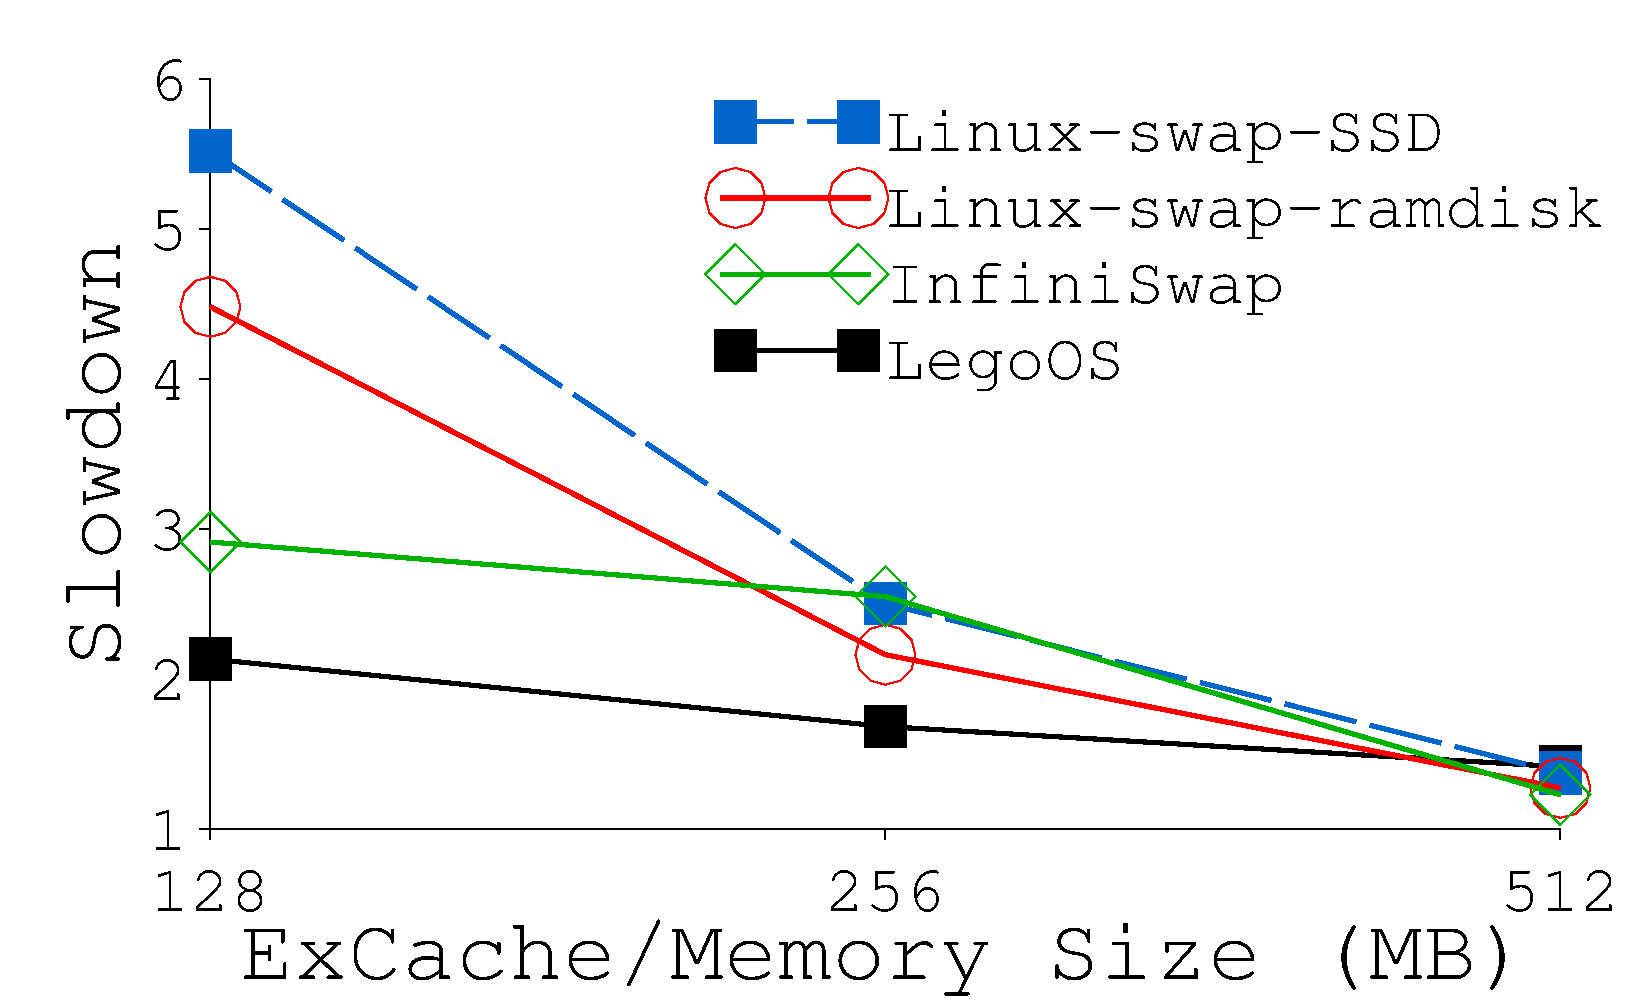
\includegraphics[width=0.5\textwidth]{lego/Figures/g_plot_LEGO_tf4.pdf}}
\caption[TensorFlow Performance.]{TensorFlow Performance.}
\label{fig-tf4}
\end{center}
\end{figure*}
}
{
\begin{figure*}[th]
\begin{center}
\centerline{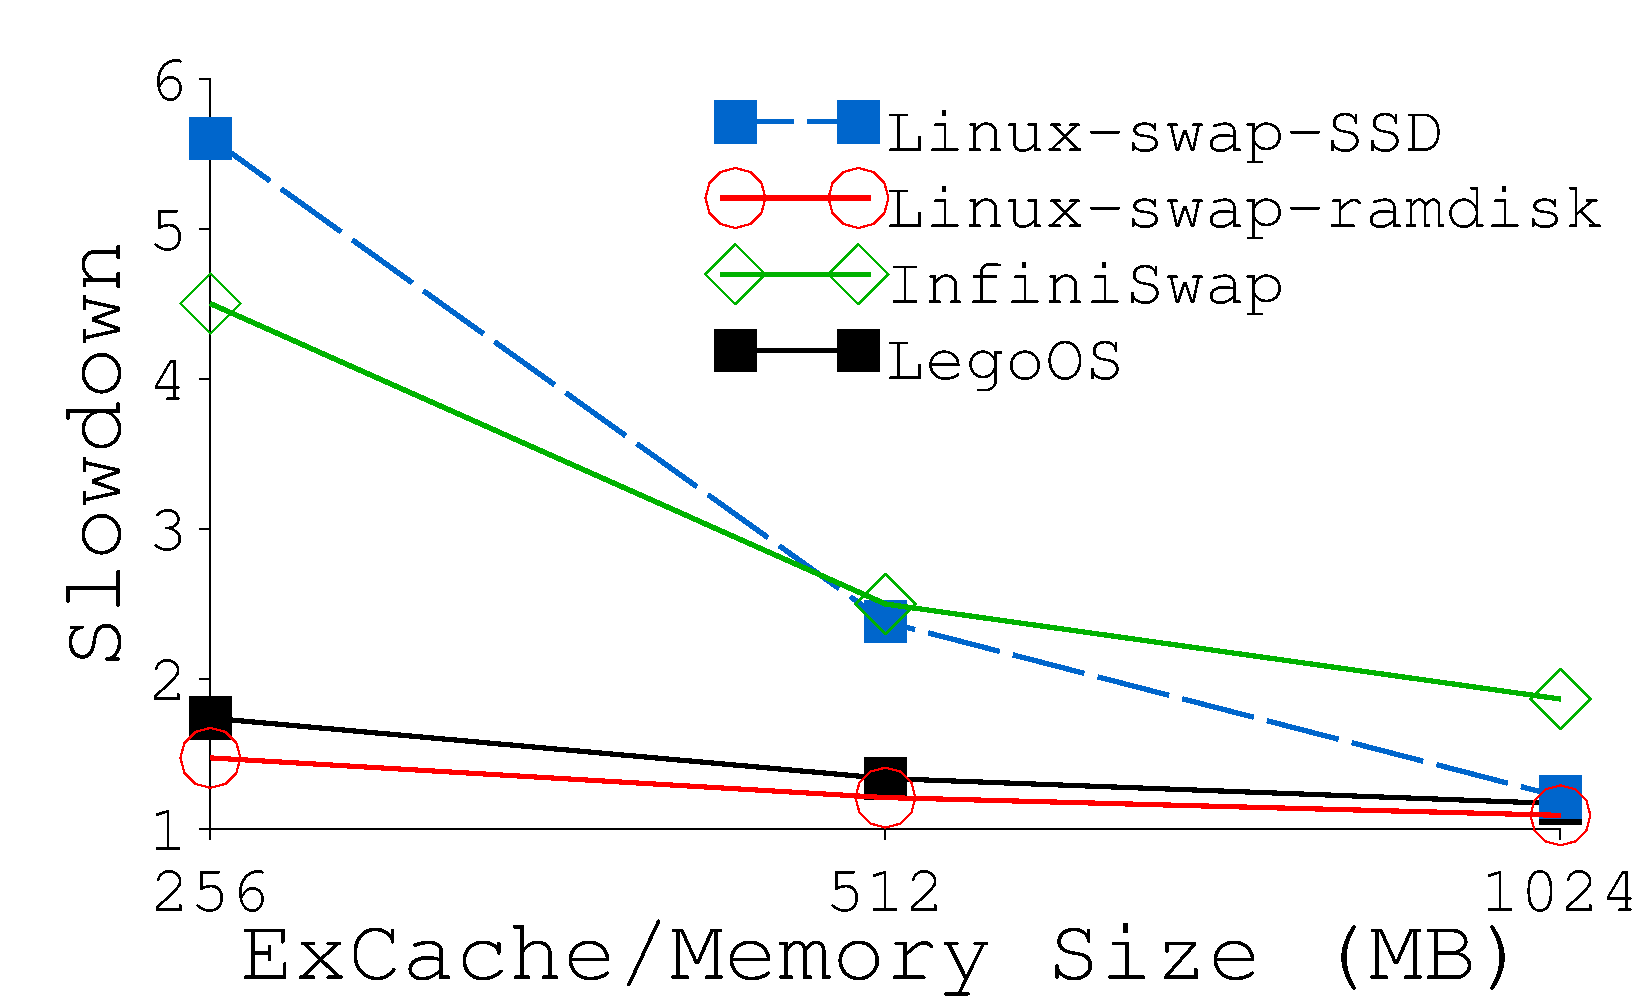
\includegraphics[width=0.5\textwidth]{lego/Figures/g_plot_LEGO_phoenix.pdf}}
\caption{Phoenix Performance.}{Phoenix Performance.}
\label{fig-phoenix}
\end{center}
\end{figure*}
}
{
\begin{figure*}[th]
\begin{center}
\centerline{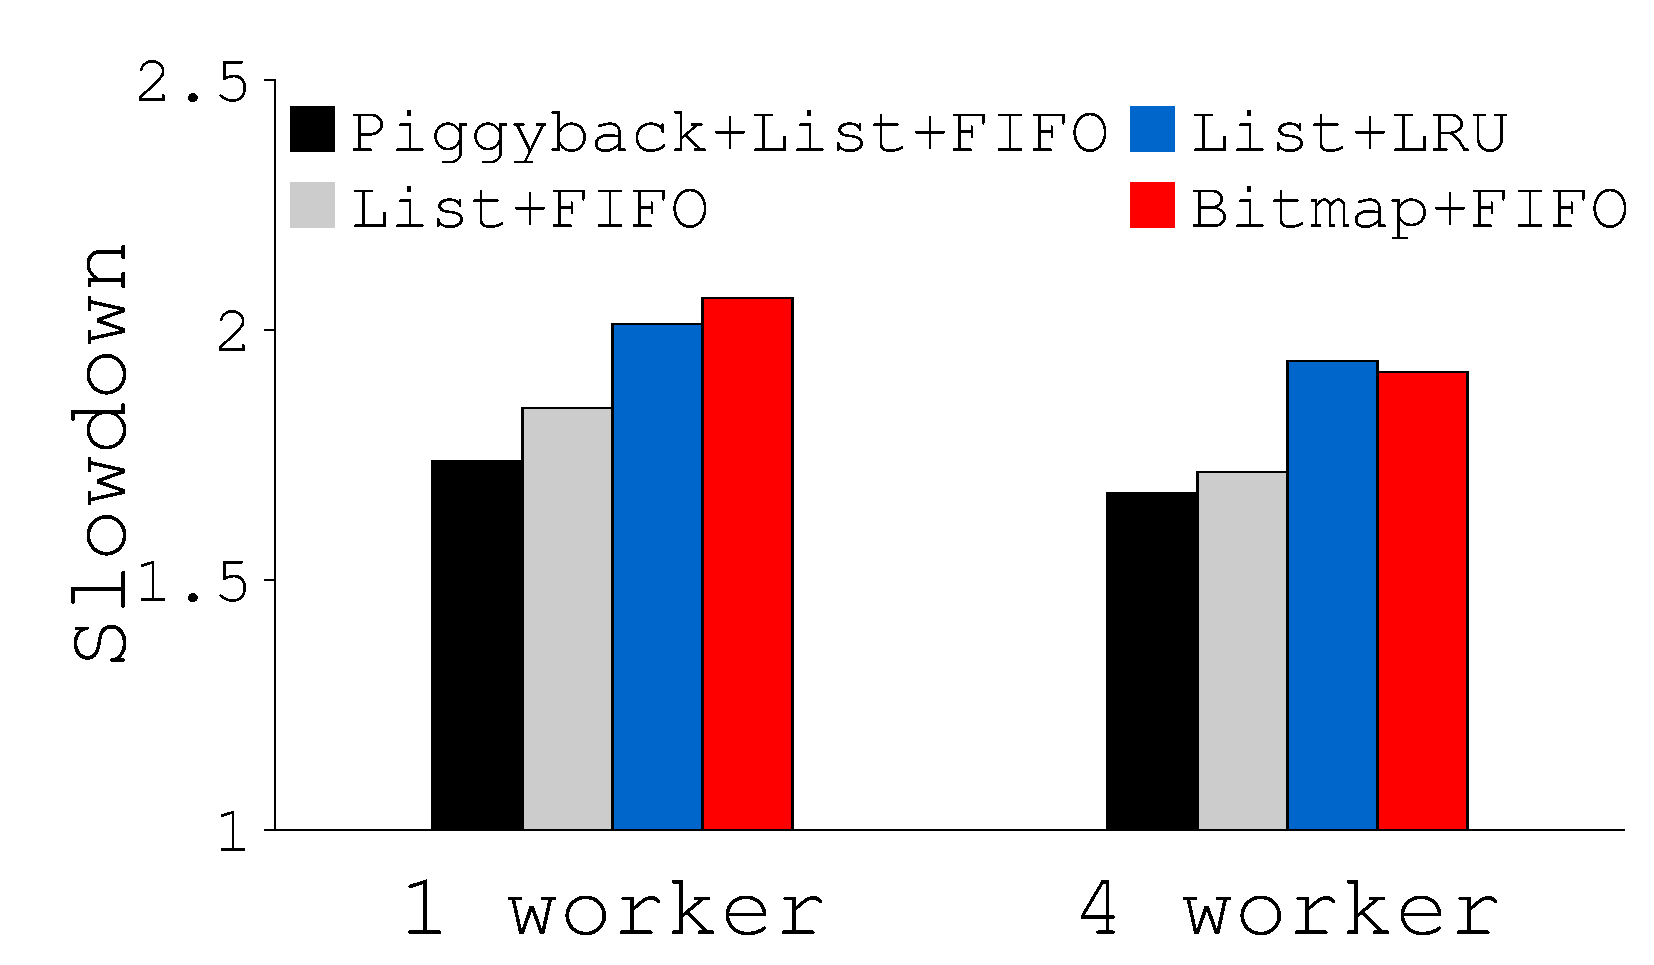
\includegraphics[width=0.5\textwidth]{lego/Figures/g_plot_LEGO_excache_tech.pdf}}
\caption{ExCache Management.}{ExCache Management.}
\label{fig-excache-opt}
\end{center}
\end{figure*}
}
{
\begin{figure*}[th]
\begin{center}
\centerline{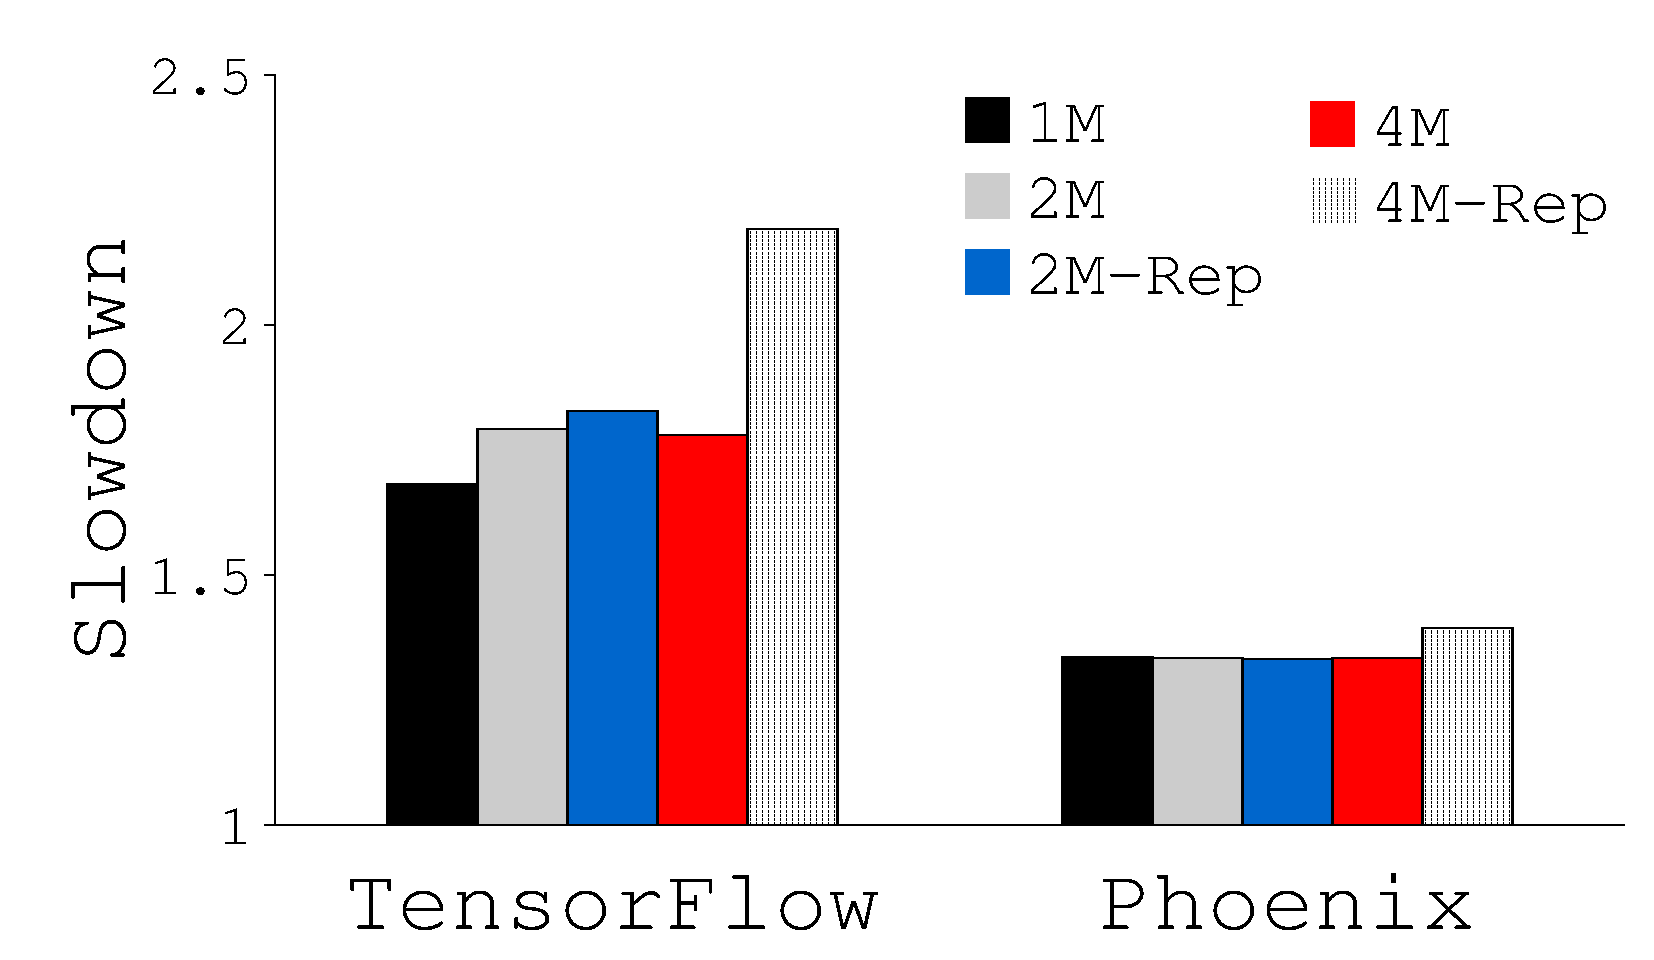
\includegraphics[width=0.5\textwidth]{lego/Figures/g_plot_LEGO_number_memory_rep.pdf}}
\caption[Memory Config.]{Memory Config.}
\label{fig-mem-rep}
\end{center}
\end{figure*}
}
\noindent{\textit{\uline{PARSEC results.}}}
We evaluated \lego\ with a set of workloads from the PARSEC benchmark suite~\cite{PARSEC},
including BlackScholes, Freqmine, and StreamCluster.
These workloads are a good representative of compute-intensive datacenter applications, 
ranging from machine-learning algorithms to streaming processing ones.
Figure~\ref{fig-parsec} presents the slowdown of \lego\ 
over single-node Linux with enough memory for the entire application working sets.
\lego\ uses one \pcomponent\ with 128\MB\ \excache,
one \mcomponent\ with one worker thread, and one \scomponent\ for all the PARSEC tests.
For each workload, we tested one and four workload threads.
StreamCluster, a streaming workload, performs the best because of its 
batching memory access pattern (each batch is around 110\MB).
BlackScholes and Freqmine perform worse because of their larger working sets (630\MB\ to 785\MB).
\lego\ performs worse with higher workload threads, 
because the single worker thread at the \mcomponent\ becomes the bottleneck to achieving higher throughput.
%This result suggests that stream processing is a good fit to \lego.
%Finally, for these PARSEC workloads, the number of \mcomponent s have no or small effects.

\subsection{Application Performance}
\label{sec:appresults}
We evaluated \lego' performance with two real, unmodified applications, 
TensorFlow~\cite{TensorFlow} and Phoenix~\cite{Ranger07-HPCA}, a single-node multi-threaded implementation of MapReduce~\cite{DeanEtAl04-MapReduce}.
TensorFlow's experiments use the Cifar-10 dataset~\cite{CIFAR-DS} and Phoenix's use a Wikipedia dataset~\cite{Wiki-DS}.
Unless otherwise stated, the base configuration used for all TensorFlow experiments
is 256\MB\ 64-way \excache, one \pcomponent, one \mcomponent, and one \scomponent.
The base configuration for Phoenix is the same as TensorFlow's with the exception that the base \excache\ size is 512\MB.
The total amount of virtual memory addresses touched in TensorFlow is 4.4\GB\ (1.75\GB\ for Phoenix).
The total working sets of the TensorFlow and Phoenix execution are 0.9\GB\ and 1.7\GB.
Our default \excache\ sizes are set as roughly 25\% of total working sets.
We ran both applications with four threads.

\noindent{\textit{\uline{Impact of \excache\ size on application performance.}}}
Figures~\ref{fig-tf4} and \ref{fig-phoenix} plot the TensorFlow and Phoenix run time comparison across 
\lego, a remote swapping system (InfiniSwap~\cite{GU17-NSDI}), 
a Linux server with a swap file in a local high-end NVMe SSD, 
and a Linux server with a swap file in local ramdisk.
All values are calculated as a slowdown to running the applications on a Linux server that have enough local resources (main memory, CPU cores, and SSD).
For systems other than \lego, we change the main memory size to the same size of \excache\ in \lego, with rest of the memory on swap file. 
With around 25\% working set, \lego\ only has a slowdown of 1.68\x\ and 1.34\x\ for TensorFlow and Phoenix
%of incurs the overhead of TensorFlow and Phoenix on \lego\ are 
compared to a monolithic Linux server that can fit all working sets in its main memory.

\lego' performance is significantly better than swapping to SSD and to remote memory 
largely because of our efficiently-implemented network stack, simplified code path compared with Linux paging subsystem,
and the optimization technique proposed in \S\ref{sec:zerofill}.
Surprisingly, it is similar or even better than swapping to local memory, even when \lego' memory accesses are across network.
This is mainly because ramdisk goes through buffer cache and incurs memory copies between the buffer cache and the in-memory swap file.

\lego' performance results are not easy to achieve and we went through rounds of design and implementation refinement.
Our network stack and RPC optimizations yield a total improvement of up to 50\%.
For example, we made all RPC server (\mcomponent's) replies {\em unsignaled} to save \mcomponent' processing time
and to increase its request handling throughput.
Another optimization we did is to piggy-back dirty cache line flush and cache miss fill into one RPC.
The optimization of the first anonymous memory access (\S\ref{sec:zerofill}) improves \lego' performance further by up to 5\%.

\noindent{\textit{\uline{\excache\ management.}}}
Apart from its size, how an \excache\ is managed can also largely affect application performance.
We first evaluated factors that could affect \excache\ hit rate and found that higher associativity improves hit rate
but the effect diminishes when going beyond 512-way.
We then focused on evaluating the miss cost of \excache, since the miss path is handled by \lego\ in our design.
We compare the two eviction policies \lego\ supports (FIFO and LRU),
two implementations of finding an empty line in an \excache\ set (linearly scan a free bitmap and fetching the head of a free list),
and one network optimization (piggyback flushing a dirty line with fetching the missing line).

Figure~\ref{fig-excache-opt} presents these comparisons with one and four \mcomponent\ worker threads. 
All tests run the Cifar-10 workload on TensorFlow with 256\MB\ 64-way \excache, one \mcomponent, and one \scomponent.
Using bitmaps for this \excache\ configuration is always worse than using free lists
because of the cost to linearly scan a whole bitmap,
and bitmaps perform even worse with higher associativity.
Surprisingly, FIFO performs better than LRU in our tests, even when LRU utilizes access locality pattern.
We attributed LRU's worse performance to the lock contention it incurs;
the kernel background thread sweeping the \excache\ locks an LRU list when adjusting the position of an entry in it,
while \excache\ miss handler thread also needs to lock the LRU list to grab its head.
Finally, the piggyback optimization works well and the combination of FIFO, free list, and piggyback yields the best performance.

{
\begin{table*}[th]\footnotesize
\begin{center}
\begin{tabular}{ l || c | c | c | c | c | c || c | c}
 & Processor & Disk & Memory  & NIC & Power & Other & Monolithic & \lego\ \\
\hline
%Unit Cost & \$6500 & \$530 & \$760 & \$360 & \$380 &\$320 & \$7400 & N/A \\
%Monolithic & 100 & (200) & (400) & (100) & (100) & 100 & 3  & \$704,200\\
%Disaggregation & 0 & 100 & 200 + 50 & 0 & 100 & 125 & 4 & \$350,600 \\

MTTF (year) & 204.3 & 33.1 & 289.9 & 538.8 & 100.5 & 27.4 & 5.8 & 6.8 - 8.7 \\
%MTTF  & &&&&&& \\

\end{tabular}
\end{center}
\vspace{-0.2in}
\mycaption{tbl-failure}{Mean Time To Failure Analysis.}
{
MTTF numbers of devices (columns 2 to 7) are obtained from~\cite{Failure-Disk-FAST07}
and MTTF values of monolithic server and \lego\ are calculated using the per-device MTTF numbers.
%Unit: year.
%MTTPF: Mean Time To Permanent (hardware) Failure, MTTF: Mean Time To (all types of hardware) Failure.
%Per-device MTTF used to calculate MTTPF are collected from Table 3 in \cite{Failure-Disk-FAST07}.
%Processor failure includes the failure of CPU, fan, and CPU heat sink (for both monolithic server and Lego).
}
%\vspace{-0.1in}
\end{table*}
%\vspace{-0.1in}
}


\noindent{\textit{\uline{Number of \mcomponent{}s and replication.}}}
Finally, we study the effect of the number of \mcomponent s and memory replication.
Figure~\ref{fig-mem-rep} plots the performance slowdown as the number of \mcomponent s increases from one to four.
Surprisingly, using more \mcomponent{}s lowers application performance by up to 6\%.
This performance drop is due to the effect of \excache\ piggyback optimization. 
When there is only one \mcomponent, flushes and misses are all between the \pcomponent\ and this \mcomponent,
thus enabling piggyback on every flush.
%the \mcomponent\ to be flushed to is always the  to fetch the missing page from.
However, when there are multiple \mcomponent{}s, \lego\ can only perform piggyback when flushes and misses are to the same \mcomponent.
%this is not true anymore. Essentially,
%multiple \mcomponent s case will involve more network RPC than one \mcomponent\ case.

We also evaluated \lego' memory replication performance in Figure~\ref{fig-mem-rep}.
Replication has a performance overhead of 2\% to 23\% (there is a constant 1\MB\ space overhead to store the backup log).
\lego\ uses the same application thread to send the replica data to the backup \mcomponent\ and then 
to the primary \mcomponent, resulting in the performance lost. 
%The performance overhead is a result of 
%We also tested synchronous replication where foreground waits for the write back of backup memory log.
%The synchronous replication scheme has an overhead of 1.2\%.

\noindent{\textit{\uline{Running multiple applications together.}}}
All our experiments so far run only one application at a time.
Now we evaluate how multiple applications perform when running them together on a \lego\ cluster.
We use a simple scenario of running one TensorFlow instance and one Phoenix instance together in two settings:
1) two \pcomponent{}s each running one instance, both accessing one \mcomponent (2P1M),
and 2) one \pcomponent\ running two instances and accessing two \mcomponent{}s (1P2M).
Both settings use one \scomponent. Figure~\ref{fig-multiapp} presents the runtime slowdown results.
We also vary the number of \mcomponent\ worker threads for the 2P1M setting (4 and 8 workers)
and the amount of \excache\ for the 1P2M setting (1\GB\ and 0.5\GB).
With 2P1M, both applications suffer from a performance drop
because their memory access requests saturate the single \mcomponent.
Using more worker threads at the \mcomponent\ improves the performance slightly.
%due to burst memory access requests from both applications resulting much higher queuing delay in the \mcomponent.
For 1P2M, application performance largely depends on \excache\ size, similar to our findings with single-application experiments.

{
\begin{figure*}[t]
\begin{center}
\centerline{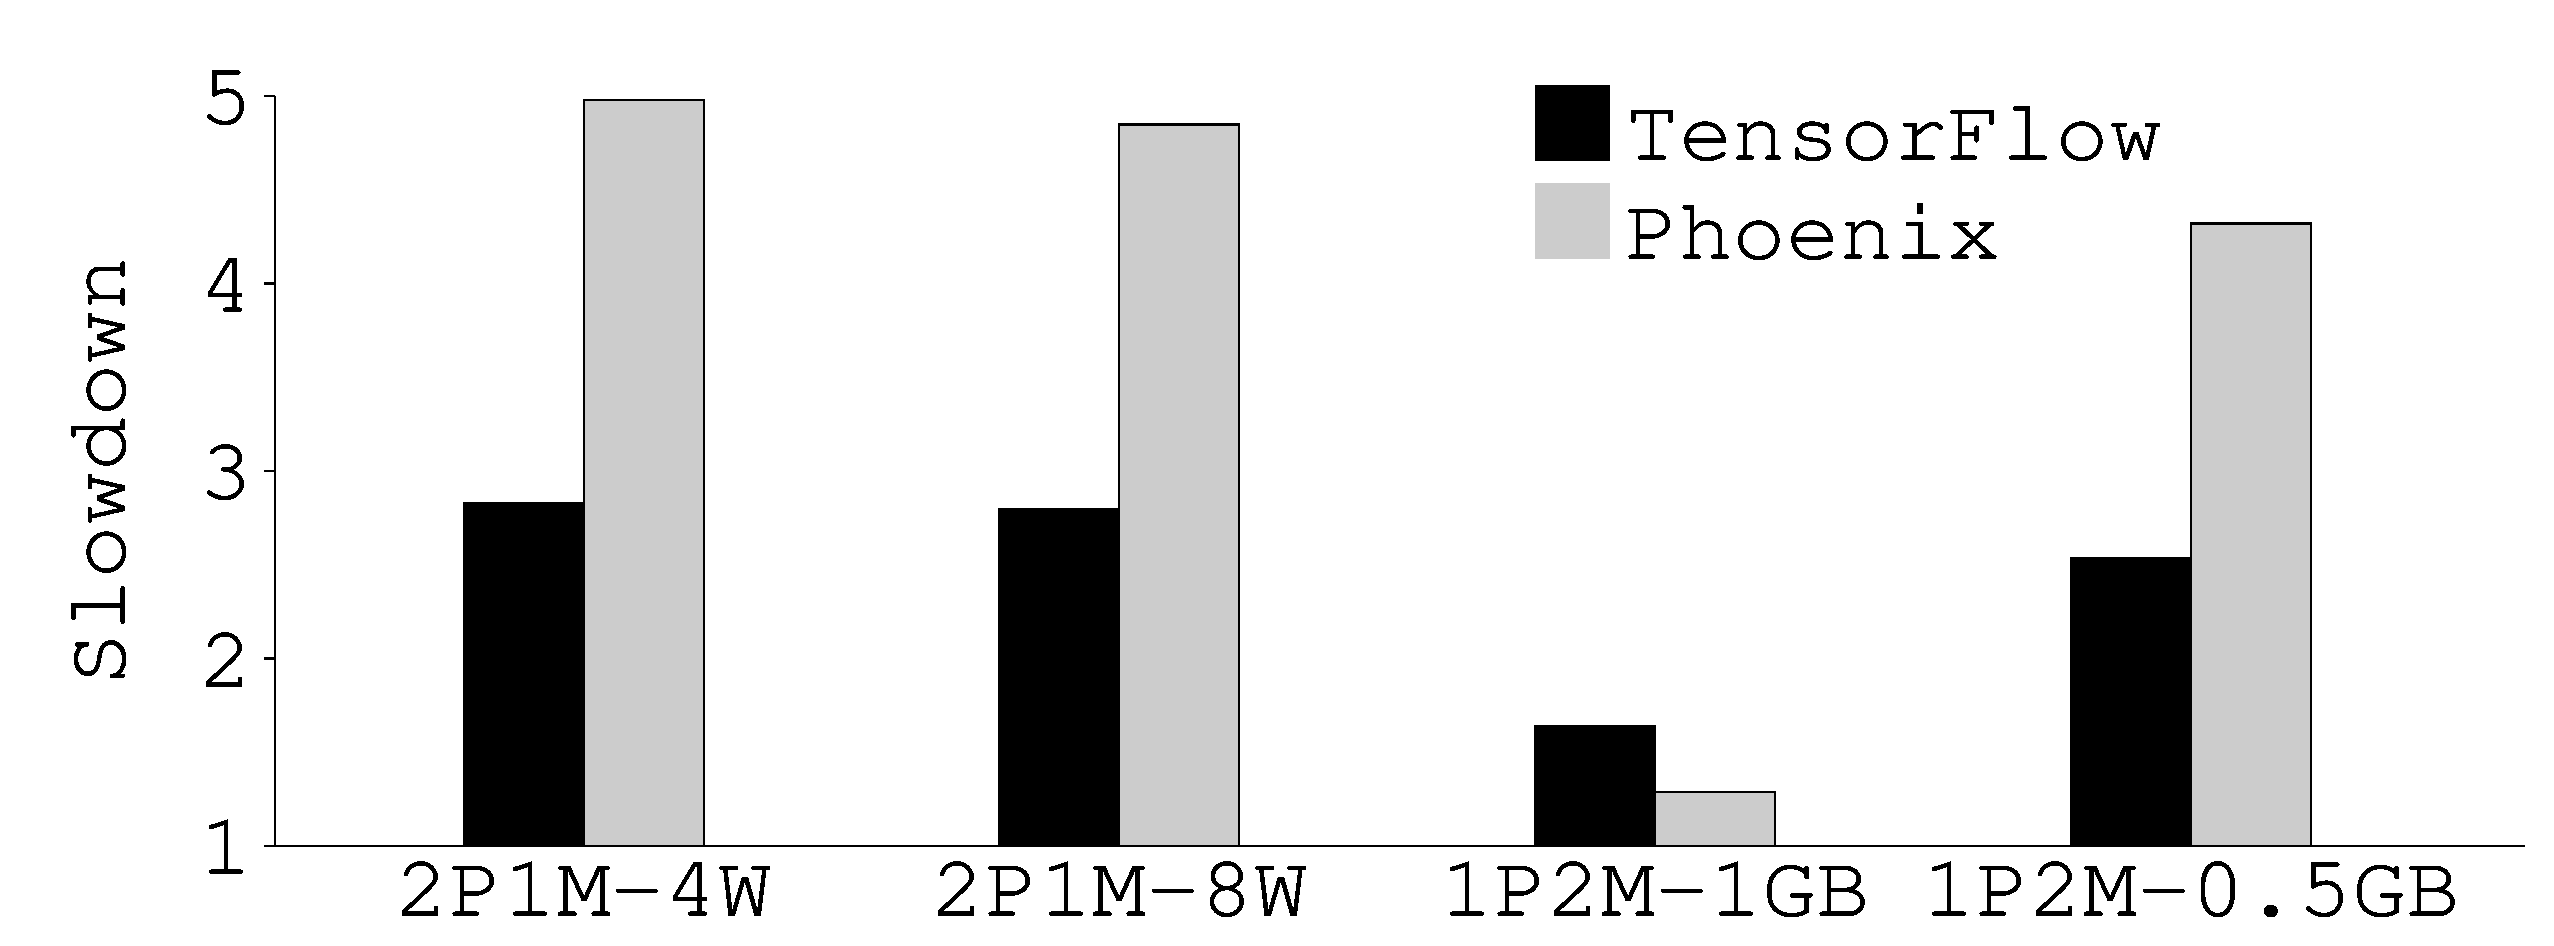
\includegraphics[width=0.6\textwidth]{lego/Figures/g_plot_LEGO_multiapp.pdf}}
\caption[Multiple Applications.]{Multiple Applications.}
\label{fig-multiapp}
\end{center}
\end{figure*}
}
%s to two applications running on same \pcomponent, 0.5G Excahce, being 19.7\% of resident memory, results
%much higher cache conflicts and evictions, furthermore reflected by 3-4 times slowdown in runtime. Meanwhile,
%1\GB\ \excache, 39.4\% of resident memory, reveals a better performance than the former.

\if 0
\subsection{Resource Packing Analysis}
\label{sec:cost}
A key advantage of a \lego\ cluster is its better resource packing compared to a monolithic cluster.
We provide a quantitative analysis of this benefits using the Google cluster trace~\cite{GoogleTrace}.
This cluster only runs VMs and the trace reports the amount of physical machines used to run the VMs 
in a 29-day period. 
The trace also provides the total amount of CPU and memory in each physical machine
and the amount of CPU and memory used by each VM.
With this set of information, we calculated the CPU and memory utilization of the whole Google cluster.

We calculate the amount of total memory and total CPU needed for a \lego\ cluster separately.
For memory, since \lego\ can freely allocate memory from any \mcomponent{}s and the allocation is performed on demand, 
we simply use the estimation of total memory required being {\small{$1+RepOvhd$}} of total memory used,
where {\small{$RepOvhd$}} is the space overhead to store the backup log for each \mcomponent.
The estimation of \lego' CPU usage is more complex.
Since \lego\ cannot split a process across \pcomponent{}s and the trace does not provide information of 
processes within a VM, we simply treat one VM as the unit of allocation.
We perform a further estimation by using a first-fit allocation algorithm to assign VMs to \pcomponent{}s 
based on available cores of \pcomponent{}s.

\fixme{will continue analysis after power outage}
\fi

\subsection{Failure Analysis}
\label{sec:failure-results}
Finally, we provide a qualitative analysis on the failure rate of a \lego\ cluster compared to a monolithic server cluster.
Table~\ref{tbl-failure} summarizes our analysis.
To measure the failure rate of a cluster, we use the metric Mean Time To (hardware) Failure (MTTF), 
the mean time to the failure of a server in a monolithic cluster
or a component in a \lego\ cluster.
Since the only real per-device failure statistics we can find are
the mean time to hardware replacement in a cluster~\cite{Failure-Disk-FAST07},
the MTTF we refer to in this study indicates the mean time to the type of 
hardware failures that require replacement.
Unlike traditional MTTF analysis, we are not able to include transient failures.
%MTTF indicates the frequency of hardware replacement in a cluster.

To calculate MTTF of a monolithic server, we first obtain the replacement frequency of different hardware devices in a server
(CPU, memory, disk, NIC, motherboard, case, power supply, fan, CPU heat sink, and other cables and connections)
from the real world (the COM1 and COM2 clusters in \cite{Failure-Disk-FAST07}).
For \lego, we envision every component to have a NIC and a power supply, 
and in addition, a \pcomponent\ to have CPU, fan, and heat sink, an \mcomponent\ to have memory, and an \scomponent\ to have a disk.
We further assume both a monolithic server and a \lego\ component to fail when any hardware devices in them fails
and the devices in them fail independently.
Thus, the MTTF can be calculated using the harmonic mean ({\em HM}) 
of the MTTF of each device.

\vspace{-0.05in}

\begin{small}
\begin{equation}
MTTF = \frac{HM_{i=0}^n(MTTF_i)}{n}
\end{equation}
\end{small}

\vspace{-0.05in}

\noindent where $n$ includes all devices in a machine/component. 

Further, when calculating MTTF of \lego, we estimate the amount of components needed in \lego\ 
to run the same applications as a monolithic cluster.
Our estimated worst case for \lego\ is to use the same amount of hardware devices 
(\ie, assuming same resource utilization as monolithic cluster).
\lego' best case is to achieve full resource utilization 
and thus requiring only about half of CPU and memory resources 
(since average CPU and memory resource utilization in monolithic server clusters is around 50\%~\cite{GoogleTrace,AliTrace}).

With better resource utilization and simplified hardware components (\eg, no motherboard),
\lego\ improves MTTF by 17\% to 49\% compared to an equivalent monolithic server cluster.

\if 0
Best case:
\begin{equation}
MTTF_{Lego} = \frac{HM(MTTF_P, MTTF_M, MTTF_S)}{3}
\end{equation}

Worst case:
\begin{equation}
MTTF_{Lego} = \frac{HM(MTTF_P/2, MTTF_M/2, MTTF_S)}{3}
\end{equation}
\fi


%% https://homes.cs.washington.edu/~arvind/papers/pcp.pdf

{
\begin{table*}[th]\footnotesize
\begin{center}
\begin{tabular}{ p{1in} | p{1.5in} |p{3.3in} | p{0.5in}}

\textbf{Goal} &
\textbf{Mechanism} &
\textbf{Description} &
\textbf{Section} \\
\hline
\hline

Connectivity            & Reliable link layer & enable connection between supernic and endpoints & XX \\
\hline
Endpoint Integration    & Endpoint shim layer & APIs and lighteweight states & XX \\
\hline
\hline

Perf & Partial NF Chaining & XXXX  & XXX \\
\hline

Perf & Service-level Parallelism & XXXX  & XXX \\
\hline

Perf & Instance-level Parallelism & XXXX  & XXX \\
\hline

Correctness & Reorder Buffer & parallel services and instances & XXX \\
\hline

Perf \& Security & Resource Partition & Partition resource to improve aggregated on-board throughput & XXX \\
\hline
\hline

Management & Softcore & Runs management plane (all policies) & XX \\
\hline

Consolidation & Packet Store & Shared central packet buffer & XX \\
\hline

Fairness & Credit Allocation & Eager and \& on-demand policies & XXX \\
\hline

Fairness & Header/PIFO Queues & XX & XXX \\
\hline

XX & NF Wrapper & XXXX & XXX \\
\hline

Security & Segmented VM & XXXX & XXX \\
\hline


PR Facility & PR Region Decoupler & Logically isolates static and dynamic PR regions, with quiescence API & XXX \\
\hline

Computation Scaling & PR-based Auto Scaling & PR can replace, add, and remove NFs during runtime & XXX \\
\hline

Computation Scaling & Bitstream Store & A table of bitstreams saved in on-board DRAM & XXX \\
\hline

Better Deployment & Bitstream AutoGen & A framework to generate wrapped bitstreams using user netlists & XXX \\
\hline


\end{tabular}
\end{center}
\mycaption{table-techniques}{Technique Summary.}
{
PR: Partial Reconfiguration.
NF: Network Function.
}
\end{table*}
}


\if 0
\section{\sysname\ Overview}
\label{sec:overview}

We walk through the key challenges and present out solutions.

\boldunderpara{Key Challenges:}
\begin{itemize}[leftmargin=0cm,itemindent=.35cm]

\myitem{C1:}
After decoupling the network, what's left at the endpoints?
And how can endpoints communicate with the NetPool?
%
\textbf{Answer:} \TODO{}
We observe that a reliable link layer is sufficient
to connect endpoints and NetPool.
We design a shim library at the endpoints.

\myitem{C2:}
How to efficiently and safely consolidate applications onto NetPool
with limited amount of resource?
%
\textbf{Answer:} \TODO{}
Scheduling: space and time sharing limited resource.
Auto Scaling: xxx.
Isolation: segmented virtual memory, XXX.
Fairness: PIFO, XXX.



\myitem{C3:}
How to design a flexible management interface so that
we can deploy, upgrade, scale applications easily?
\textbf{Answer:}
Although FPGA enables in field reconfiguration,
it is far from a complete solution.
In response, \sysname\ makes a clean separation between the management and data plane.
The management plane makes decisions based on runtime policies
and react to real time traffic load. The data plane simply follows
the management plane's instructions and adapts its computation layout.
We build the management plane using C running at softcores.
As a result, \sysname\ has software-alike configurability
while able to run at raw hardware speed.

\myitem{C4:} The NetPool adds another hop in the path and is
shared by many applications, how to ensure low latency and high throughput?
%
\textbf{Answer:}
Latency: we make two technical contributions.
a) to optimize the common case, we propose \textif{partial chaining}
to shorten the connection latency between chained functions.
b) we use service-level parallelism to shorten critical path.
Throughput:
we use \textit{resource partitioning} and ensure SuperNIC's system
component (e.g., packet scheduler) is able to sustain peak throughput.
\yizhou{partitioning maybe beneficial for side channels}.
When consolidated computation exceeds SuperNIC's capacity,
we use either time- or space-sharing to multiplex resource.
As a result, the execution latency build up.
We trade some extra latency for the consolidation benefits.
Luckily, we obverse that datacenter traffic is bursty and mostly underutilized,
thus peak load scenario is rare.

\myitem{C5:} Failure.
The failure domain is enlarged.
Shall we handle it? If so, how?
Make endpoints multi-homed. Add another link
to switch or to another sNIC.

\yizhou{other challenges: tail latency. security, side channels, programming framework.}

\yizhou{for latency part: it would be great to say:
we obverse the average chain length is XXX,
and we find XX\% traffic will traverse N NFs.
Also, in our eval, during low load, we found offloading transport and NF
to SuperNIC actually improves latency compared to baselin (running transport
on CPU or smartnic like bluefield.)
}

\end{itemize}
%
\\


\textbf{Features}

1. Distributed setup.
A resource pool has set of connected SuperNIC, in mesh or others.
3 planes.
Traffic can bounce among SuperNICs.
Load balancing. (\TODO{depends.})

2. Resource consolidation and abstraction groups.
Describe how end points can choose to offload whatever to supernic,
they could enjoy flexible combo. (this is essentially our Abstraction discussion earlier.)

3. New smartnic architecture.
Highlight prior archs, esp PANIC, show the difference.
Our arch has the benefits of both worlds (we have a diagram for this).

4. Packet Processing Parallelism.
We introduce service-level and instance-level parallelism.
And to ensure ordering, we introduce Reorder Buffer, a mechanism that XXX.

5. Runtime NF Scheduling and scaling, time and space sharing.
We closely monitor NF status and does automatic NF scheduling and scaling

6. Performance Isolation and Protection.
We have virtual memory interface for on-board memory.
We use PIFO and other things to control bandwidth etc.
\fi

\section{\sysname\ Design Yizhou}
\label{sec:design}

\subsection{Overview}

SuperNIC's innovation comes from two parts, the board-level design and the distributed design.

\subsubsection{At Board-Level}

We adopt PANIC’s architecture as our baseline.
Its design enables resource consolidation and flexible NF chaining.
Despite its advantages over traditional RMT, Pipeline, and SoC-based SmartNICs, PANIC suffers from long chaining latency and cannot scale resources.

We propose three techniques to improve this state-of-the-art SmartNIC architecture, namely, 1) traffic-aware NF merging, 2) eager credit allocation scheduling, 3) on-demand scheduling and auto-scaling. These techniques are crucial for reducing latency and enable flexible consolidation. We will cover the details later. (NF merging has two benefits: reduce latency, and increase slot resource utilization while reducing the pressure on the xbar. We need experiments to show.)

In addition, we introduce a softcore (could be a real SoC in the future)
to run the management and control plane tasks.
Our microservice-style software is partitioned into \texttt{agents}.
Each agent is responsible for one particular task, e.g., we currently have monitoring agent, auto-scaling agent, Inter-SuperNIC agent, PR agent, and so on.
It presents a shell-alike interface hence administrates can control SuperNIC via simple commands. 

In all, a single SuperNIC supports multi-tenancy chaining,
traffic-aware NF merging, on-demand scheduling, and auto scaling.
It presents flexible policies with a clean separation of data and management/control planes.

\subsubsection{At Distributed-Level}

A single SuperNIC has limited resources and may become the computation bottleneck during peak load.
To tackle this issue, we leverage the fact that SuperNICs under one ToR are
connected in a ring or a mesh.
We \textit{logically} group such a pool of physically distributed SuperNICs as one giant computation entity.
Within the pool, SuperNICs are able to auto-scale, migrate, and balance computation among each other.

We offer two-level auto-scaling, in which a certain computation offload
can not only scale-up within one SuperNIC
but also scale-out across SuperNICs.
On top of it, SuperNICs can migrate computation and balance traffic on demand.

These designs are possible because of the following components.
First, each SuperNIC board has extensive monitoring facilities collecting runtime statistics for software agents to consume and make decisions using flexible policies.
Second, our fast PR mechanism serves as the basis.
Third, we deploys a hardware routing agent to help re-route traffic.

\subsection{Physical Connections}

\textit{Endpoints and Link Layer}.
We need to describe what's the minimum setting required at the endpoint side. The minimum setting is used when the whole transport and NF are moved to SuperNIC.
The minimum setting should include: a) a reliable link layer, with one-hop flow control, error detection and correction. b) a shim layer exposed to applications. this layer needs to save at least the connection IDs.
I'm a bit worried about the error correction part - what if we cannot guarantee
100\% error-free, then what's the guarantee we offer to endpoints.
We had discussion on this part before, e.g., expose bit error as network failure.

\subsection{On-chip Architecture}

\yizhou{Overview. Add a figure.}

\subsubsection{Parser}
Each RX port has a Parser attached. All parsers share a service chain store.
The parser uses Match-Action-Table style to generate a runtime
descriptor for each packet.
This descriptor is a metadata placeholder, includes XXX.

\subsubsection{Central Scheduler}

\yizhou{Deserves a zoom-in figure.}

\textbf{On-demand and eager credit management}:
The classical pull and push model proposed by
Click (used by PANIC) is designed for single element/NF.
With a NF chain, especially consider the extra cost
of going back to Scheduler or going across xbar,
it is beneficial to favor push over pull.
Mapping to our model, we propose on-demand
and eager credit management.

On-demand credit allocation:
If a packet is going to use a NF, the packet must allocate credit right before traversing the NF.
Hence, if a packet needs to traverse a NF chain, the packet must go back to the central scheduler to
allocate credit for the next NF in the chain. 

Eager credit allocation:
The packet can pre-allocate credits for services it going to use.
Hence, if a packet wants to traverse a NF chain, the packet would 
allocate credits for all NFs in the chain.
Implication: a packet will wait until all NFs in a chain have available credits.

Eager credit pre-allocate resources, lower latency, but may have poor resource utilization.
We think the eager should be the default policy during low load.
We should switch to on-demand when load spikes.

\subsubsection{Parallelism}
Reorder buffer.

Three-level parallelism.
1) pipeline level.
2) fine-grained, needs help from a PL framework.
3) service-level, coarse-grained. Either manual linking, or use a high-level scripting language like Click.
4) instance-level, among instances of the same service.

For now, 1) come from user, 2) is our future work,
We can do 3), manually. We have to do 4).
Both 3 and 4 need the help of ROB.

\yizhou{we could briefly mention that this can benefit from a programming framework. The PL part is deferred to the Discussion section.}

\subsubsection{Service Scheduling}
Mechanism: we use counters. rely on fpga PR, a softcore.
Policy: based on counters? once it exceeds/lowers than XXX, we do YYY.

\subsubsection{Abstraction Groups}

0. Wrapper, and other facilities: slot, PR wrapper, etc.

1. Transports (what about congestion control?)
2. Network Function

\if 0
\subsubsection{NF Shell}
We expose a standard shell abstraction to each running NF.
The shell is analogous to a system call interface,
through which NF will communicate with the rest of SuperNIC.
The shell has several standard signals such as fixed clock (250 MHz),
a pair of network interface, memory access interface, and control signals. Amazon F1 has a similar shell.
\fi

\subsubsection{Security Measures}
Consolidating resource means we need security measures.
1) NFs are only allowed to access shared resource via a fixed set of interfaces provided by shell. This reduced the exposed attack surface.
2) On-board memory employs a simple segment-based permission checking.
3) From FPGA's perspective, the generation framework (we should have a section describing what's this) would do security checks during compilation time, to filter FPGA side-channels designs (bunch papers on this).

\subsection{Distributed SuperNICs}

\subsubsection{Scale-out}
\subsubsection{Migration}
\subsubsection{Hardware Routing Agent}


%\section{Discussion}

\subsection{Programming Model}
Couple points.
1) why we need such a PL model?
2) what's in this PL model?
3) the challenges and benefits of designing/using this PL model?

We could benefit from having a programming framework, like ClickNP, the ones
that provide APIs to do packet processing. Through these APIs,
SuperNIC can do better scheduling etc.
We do not have such model yet.
Ideally, such model can be:
1) a way to describe services, their linking etc.
And SuperNIC is able to infer better NF merging and runtime scheduling policies.
2) a set of shell interfaces through which NFs interact with SuperNIC.

Also its worth mentioning: it is user/system's responsibility to partition
the function among endpoints and SuperNIC. 

\subsection{Failure}

We restrict out discussion to transient failures.
We assume permanent failures are rare.
SuperNIC adds back fate-sharing failure domain (all the connected devices and the SuperNIC). It is making failure handling a bit worse than a full disaggregation model.

Ideally, we want SuperNIC be able to physically isolate its on-board
failure domains, possibly by using different power supplies and chips.
For example, the board has two domains, one pass-through and one computation domain.
The latter hosts all logic and softcore.
If the latter fails, SuperNIC is still able to route traffic via the pass-through domain hence the connected
devices are still reachable from others.

\subsection{Security and FPGA Side-Channels}

We ensure security by properly isolate resources.
FPGA side-channels are possible, but they can be prevented
during compile time by checking user logic.
Most malicious FPGA programs have a certain signature logic.

%\section{Related Work}
\label{sec:lego:related}

\textbf{Hardware Resource Disaggregation.}
There have been a few hardware disaggregation proposals from academia and industry,
including Firebox~\cite{FireBox-FASTKeynote}, HP "The Machine"~\cite{HP-TheMachine,HP-MemoryOS}, dRedBox~\cite{dRedBox-DATE},
and IBM Composable System~\cite{IBM-Composable}.
Among them, dRedBox and IBM Composable System package hardware resources in one big case 
and connect them with buses like PCIe.
The Machine's scale is a rack and it connects SoCs with NVMs with a specialized coherent network.
FireBox is an early-stage project and is likely to use high-radix switches to connect  customized devices.
The disaggregated cluster we envision to run \lego\ on is one that hosts hundreds to thousands of
non-coherent, heterogeneous hardware devices, connected with a commodity network.

\textbf{Memory Disaggregation and Remote memory.}
Lim \etal\ first proposed the concept of hardware disaggregated memory
with two models of disaggregated memory: using it as network swap device 
and transparently accessing it through memory instructions~\cite{Lim09-disaggregate,Lim12-HPCA}.
Their hardware models still use a monolithic server at the local side. 
\lego' hardware model separates processor and memory completely. %is different.
%
Another set of recent projects utilize remote memory without changing 
monolithic servers~\cite{Dragojevic14-FaRM,Nelson15-ATC,remote-region-atc18,GU17-NSDI,Novakovic16-SOCC,hotpot-socc17}.
For example, InfiniSwap~\cite{GU17-NSDI} transparently swaps local memory to remote memory via RDMA.
These remote memory systems help improve the memory resource packing in a cluster.
However, as discussed in \S\ref{sec:lego:motivation}, unlike \lego, these solutions cannot solve other limitations 
of monolithic servers like the lack of hardware heterogeneity and elasticity. 

\textbf{Storage Disaggregation.}
Cloud vendors usually provision storage at different physical machines~\cite{deepview-nsdi18,url:aws-storage,url:vmware-vSAN}.
Remote access to hard disks is a common practice, because their high latency and low throughput
can easily hide network overhead~\cite{petal-asplos96,blizzard-nsdi14,Parallax-hotos15,Legtchenko-hotstorage17}.
While disaggregating high-performance flash is a more challenging task~\cite{FlashDisaggregation,url:facebook-lighting}.
Systems such as ReFlex~\cite{ReFlex}, Decibel~\cite{decibel-nsdi17}, and PolarFS~\cite{PolarFS-VLDB18},
tightly integrate network and storage layers to minimize software overhead in the face of fast hardware.
Although storage disaggregation is not our main focus now,
we believe those techniques can be realized in future \lego\ easily.

\textbf{Multi-Kernel and Multi-Instance OSes.}
Multi-kernel OSes like Barrelfish~\cite{Baumann-SOSP09,Barrelfish-DC}, Helios~\cite{Helios-SOSP}, Hive~\cite{Hive-SOSP}, and fos~\cite{fos-SOCC}
run a small kernel on each core or programmable device in a monolithic server,
and they use message passing to communicate across their internal kernels.
Similarly, multi-instance OSes like Popcorn~\cite{popcorn-eurosys15} and Pisces~\cite{Pisces-hpdc15} run multiple Linux kernel instances
on different cores in a machine. % to provide heterogeneous support and performance isolation.
Different from these OSes, \lego\ runs on and manages a distributed set of hardware devices;
it manages distributed hardware resources using a two-level approach and handles device failures (currently only \mcomponent).
In addition, \lego\ differs from these OSes in how it splits OS functionalities, where it executes the split kernels,
and how it performs message passing across components.
Different from multi-kernels' message passing mechanisms which are performed over buses or using shared memory in a server, 
\lego' message passing is performed using a customized RDMA-based RPC stack over InfiniBand or RoCE network.
Like \lego, fos~\cite{fos-SOCC} separates OS functionalities and run them on different processor cores that share main memory.
Helios~\cite{Helios-SOSP} runs {\em satellite kernels} on heterogeneous cores and programmable NICs that are not cache-coherent.
We took a step further by disseminating OS functionalities to run on individual, network-attached hardware devices. % and run split kernel at hardware controllers.
Moreover, \lego\ is the first OS that separates memory and process management and runs virtual memory system completely at network-attached memory devices.

\textbf{Distributed OSes.}
There have been several distributed OSes built in late 80s and early 90s~\cite{Amoeba-Status,Amoeba-Experience,Sprite,MOSIX,V-System,Accent-SOSP,DEMOS-SOSP,Charlotte}.
Many of them aim to appear as a single machine to users and focus on improving inter-node IPCs. 
Among them, the most closely related one is Amoeba~\cite{Amoeba-Status,Amoeba-Experience}.
It organizes a cluster into a shared process pool and disaggregated specialized servers.
Unlike Amoeba, \lego\ further separates memory from processors and different hardware components are
loosely coupled and can be heterogeneous instead of as a homogeneous pool.
There are also few emerging proposals to build distributed OSes in datacenters~\cite{Wolfgang-hotcloud18,Schwarzkopf-apsys13}, 
\eg, to reduce the performance overhead of middleware.
\lego\ achieves the same benefits of minimal middleware layers by only 
having \lego\ as the system management software for a disaggregated cluster
and using the lightweight \vnode\ mechanism.

\section{Conclusion}
\label{sec:snic:conclude}

We propose network disaggregation and consolidation by building SuperNIC, a new networking device specifically for a disaggregated datacenter.
Our FPGA prototype demonstrates the performance and cost benefits of \snic.
Our experience also reveals many new challenges in a new networking design space that could guide future researchers.

\section{Acknowledgments}
Chapter 5, in part, has been submitted for publication of the material as it may appear in Yizhou Shan, Will Lin, Ryan Kosta, Arvind Krishnamurthy, Yiying Zhang, ``Disaggregating and Consolidating Network Functionalities with SuperNIC'', \textit{arXiv, 2022}. The dissertation author was the primary investigator and author of this paper.

%

%\documentclass[pageno]{jpaper}

%replace XXX with the submission number you are given from the ASPLOS submission site.
%\newcommand{\asplossubmissionnumber}{968}

%\usepackage[normalem]{ulem}
%
\newcommand{\mycaption}[3]{\beforecaption\caption{\label{#1}{\bf #2} \em\small #3}\aftercaption}

\newcommand{\BigO}[1]{${\cal O}(#1)$}
\newcommand{\BigOmega}[1]{$\Omega(#1)$}
\newcommand{\BigTheta}[1]{$\Theta(#1)$}

% only foreign words should be italicized... (example given should not)
\newcommand{\eg}{\textit{e.g.}}
\newcommand{\ie}{\textit{i.e.}}
\newcommand{\etal}{\textit{et al.}}
\newcommand{\etc}{\textit{etc.}}
\newcommand{\adhoc}{\textit{ad hoc}}

% units
\newcommand{\KB}{\,KB}
\newcommand{\MB}{\,MB}
\newcommand{\GB}{\,GB}
\newcommand{\TB}{\,TB}
\newcommand{\MBs}{\,MB/s}
\newcommand{\KBs}{\,KB/s}
\newcommand{\Kbs}{\,Kbit/s}
\newcommand{\mbs}{\,Mbit/s}
\newcommand{\mus}{\mbox{\,$\mu s$}}
\newcommand{\ms}{\mbox{\,$ms$}}

\renewcommand{\em}{\it}
\newcommand{\x}{$\times$}

% lego
\newcommand{\splitkernel}{splitkernel}
\newcommand{\lego}{LegoOS}
\newcommand{\ib}{IB}
\newcommand{\ibverbs}{IB-Verbs}
\newcommand{\rdma}{RDMA}
\newcommand{\dcrack}{DC-Rack}
\newcommand{\vnode}{vNode}
\newcommand{\vip}{vIP}
\newcommand{\vmount}{vMount}
\newcommand{\mmap}{{\texttt{mmap}}}
\newcommand{\munmap}{{\texttt{munmap}}}
\newcommand{\mremap}{{\texttt{mremap}}}
\newcommand{\grm}{GRM}
\newcommand{\gmm}{GMM}
\newcommand{\gsm}{GSM}
\newcommand{\gpm}{GPM}
\newcommand{\excache}{ExCache}
\newcommand{\vicache}{VtmCache}
\newcommand{\vregion}{vRegion}
\newcommand{\microos}{monitor}
%\newcommand{\microos}{$\mu$OS}
\newcommand{\brk}{{\texttt{brk}}}
\newcommand{\pcomponent}{pComponent}
\newcommand{\mcomponent}{mComponent}
\newcommand{\scomponent}{sComponent}

% dsnvm
\newcommand{\dsnvm}{DSPM}
\newcommand{\dsm}{DSM}
\newcommand{\nvm}{PM}
\newcommand{\hotpot}{Hotpot}
\newcommand{\mrmw}{MRMW}
\newcommand{\mrsw}{MRSW}
\newcommand{\wfetch}{FETCH}
\newcommand{\cd}{CD}
\newcommand{\dr}{DR}
\newcommand{\on}{ON}
\newcommand{\dn}{DN}
\newcommand{\xn}{CN}
\newcommand{\master}{MN}
\newcommand{\xactid}{CID}
\newcommand{\dirty}{dirty}
\newcommand{\committed}{committed}
\newcommand{\redundant}{redundant}
\newcommand{\ib}{IB}
\newcommand{\sendreply}{\texttt{send-reply}}
\newcommand{\atomicsendreply}{\texttt{atomic-send-reply}}
\newcommand{\multisendreply}{\texttt{multicast-send-reply}}
\newcommand{\journaled}{JOURNALED}
\newcommand{\fsyncsafe}{FSYNC\_SAFE}
\newcommand{\X}{{$\times$}}
\newcommand{\pmfs}{PMFS}
\newcommand{\tmpfs}{tmpfs}
\newcommand{\Octopus}{Octopus}
\newcommand{\Mojim}{Mojim}
\newcommand{\dsmnoxact}{DSM-NoXact}
\newcommand{\dsmxact}{DSM-Xact}
\newcommand{\clflush}{\texttt{clflush}}
\newcommand{\pcommit}{\texttt{pcommit}}
\newcommand{\mfence}{\texttt{mfence}}
\newcommand{\sfence}{\texttt{sfence}}
\newcommand{\ra}{\textbf{R1.a}}
\newcommand{\rb}{\textbf{R1.b}}
\newcommand{\rcs}{\textbf{R2.a}}
\newcommand{\rcm}{\textbf{R2.b}}
\newcommand{\rdr}{\textbf{R3.r}}
\newcommand{\rdu}{\textbf{R3.u}}
\newcommand{\re}{\textbf{R3}}
\newcommand{\rf}{\textbf{R4}}

%
\newcommand{\mm}{mm$^2$}
\newcommand{\figtitle}[1]{\textbf{#1}}
\newcommand{\us}{$\mu$s}
\newcommand{\fixme}[1]{{\color{red}\textbf{#1}}}

\definecolor{pink}{rgb}{1.0,0.47,0.6}
\newcommand{\adrian}[1]{{\color{green}\textbf{#1}}}
\newcommand{\laura}[1]{{\color{pink}\textbf{#1}}}
\newcommand{\joel}[1]{{\color{red}\textbf{#1}}}
\newcommand{\ameen}[1]{{\color{blue}\textbf{#1}}}
\newcommand{\arup}[1]{{\color{yellow}\textbf{#1}}}
\newcommand{\hungwei}[1]{{\color{purple}\textbf{#1}}}


\newcommand{\note}[2]{\fixme{$\ll$ #1 $\gg$ #2}}

\newcommand{\myitem}[1]{\item \textbf{#1}}

\lstloadlanguages{% Check Dokumentation for further languages ...
        %[Visual]Basic
        %Pascal
        C
        %C++
        %XML
        %HTML
        %Java
}

\lstdefinestyle{customc}{
  belowcaptionskip=1\baselineskip,
  breaklines=true,
  frame=b,
  xleftmargin=\parindent,
  language=C,
  showstringspaces=false,
  basicstyle=\scriptsize\ttfamily,
  keywordstyle=\bfseries\color{green!40!black},
  commentstyle=\itshape\color{purple!40!black},
  identifierstyle=\color{blue},
  stringstyle=\color{red},
}
\lstset{escapechar=@,style=customc}

%\usepackage[numbers,sort]{natbib}

%\begin{document}

\title{Clio: A Hardware-Software Co-Designed Disaggregated Memory System \\ \textbf{Extended Abstract}\vspace{-0.3in}}

\date{}

\maketitle

\thispagestyle{empty}

%\section{Introduction and Motivation}
%\label{sec:intro}






\section{Motivation}

Modern data-center applications like graph computing, data analytics, and deep learning have increasing demand for access to large amounts of memory~\cite{FastSwap}.
Unfortunately, servers are facing {\em memory capacity walls} because of pin, space, and power limitations~\cite{HP-MemoryEvol,ITRS14,MemoryWall95}.
Going forward, it is imperative for datacenters to seek solutions that can go beyond what a (local) machine can offer, \ie, using remote memory.
At the same time, data centers are seeing the needs from management and resource utilization perspectives
to {\em disaggregate} resources~\cite{Ali-SinglesDay,SnowFlake-NSDI20,FB1}\textemdash separating hardware resources into different network-attached pools 
that can be scaled and managed independently.
These real needs have pushed the idea of memory disaggregation ({\em \md} for short):
organizing computation and memory resources as two separate network-attached
pools, one with compute nodes ({\em CN}s) and one with memory nodes ({\em MN}s).

\section{Limitations of the State of the Art}
So far, \md\ research has all taken one of two approaches,
building/emulating \MN{}s with either regular servers~\cite{AIFM,InfiniSwap,FastSwap,Shan18-OSDI,zombieland} 
or raw memory devices with no processing power~\cite{Tsai20-ATC,Lim09-disaggregate,Lim12-HPCA,HP-TheMachine}.
%,ATC21Paper
%\textit{Is it possible to build \MN{}s without a server}, as promised by the original proposal of \md~\cite{Lim09-disaggregate,Shan18-OSDI}?
The fundamental issues of server-based approaches such as RDMA-based systems are the monetary cost of a host server and the inherent performance and scalability limitations caused by the way NICs interact with the host server's virtual memory system.
Raw-device-based solutions have low costs.
However, they introduce performance, security, and management problems
because when \MN{}s have no processing power, all the data and control planes have to be handled at \CN{}s~\cite{Tsai20-ATC}.
%\MN{}s become too ``dumb'' and low level when removing its processing power altogether.
%overhead of root cause why RDMA is unfit for \md\ is that it is designed to work around a host server,
%and traditional servers' virtual memory system is not designed for \md.
%Contrary to server-based \md\ solutions, \pdm\ is another extreme where there is no processing at all at \MN{}s.
%The root cause of \pdm's various performance, security, and management problems is exactly this: 
%\MN{}s are too ``dumb'' and low level.

%From the above discussion, we find that both server-based \md\ and raw physical \md\ have their limitations.
Server-based \MN{}s and \MN{}s with no processing power are two extreme approaches of building \MN{}s.
We seek a sweet spot in the middle by proposing a hardware-based \md\ solution that has the right amount of processing power at \MN{}s.
%for the right type of \MN{} management system.
%To mitigate RDMA's various issues for \md, one could try to improve RDMA's hardware design or add a software layer to work around RDMA's problems.
%This paper takes a different approach by starting
Furthermore, we take a clean-slate approach by starting from the requirements of \md\
and designing a \md-native system.
%LegoOS is the only existing work that also proposes a .
%Unfortunately, LegoOS still uses server software and the RDMA network to emulate its hardware design, leaving all the research questions we ask in this paper unanswered.

\section{Key Insights and Proposal}

{
\begin{figure*}[th]
\begin{subfigure}{1.7in}
\begin{center}
\centerline{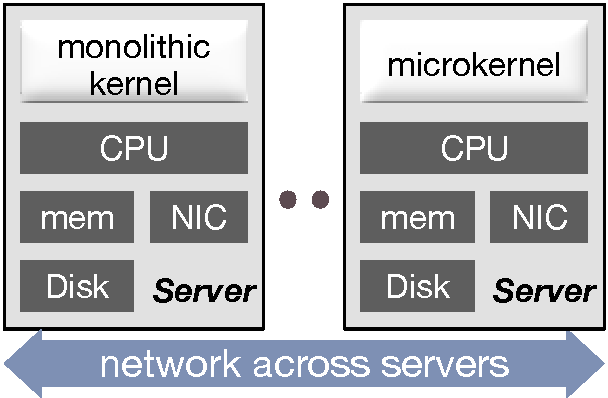
\includegraphics[width=1.7in]{lego/Figures/monolithic-arch.pdf}}
\caption[Monolithic OS.]{OSes Designed for Monolithic Servers.}
\label{fig-monolithic}
\end{center}
\end{subfigure}
\begin{minipage}{0.05in}
\hspace{0.05in}
\end{minipage}
\begin{subfigure}{1.8in}
\begin{center}
\centerline{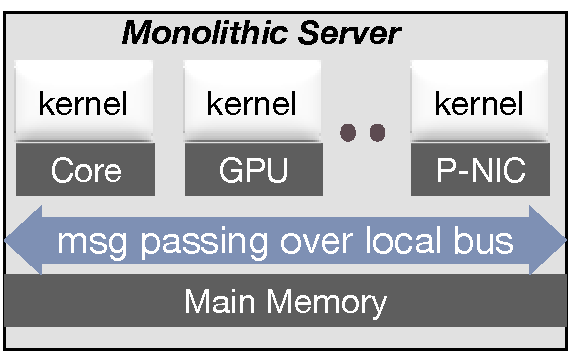
\includegraphics[width=1.8in]{lego/Figures/multikernel-arch.pdf}}
\caption[Multikernel Architecture.]{Multi-kernel Architecture. \small{P-NIC: programmable NIC.}}
\label{fig-multikernel}
\end{center}
\end{subfigure}
\begin{minipage}{0.05in}
\hspace{0.05in}
\end{minipage}
\begin{subfigure}{2.5in}
\begin{center}
\centerline{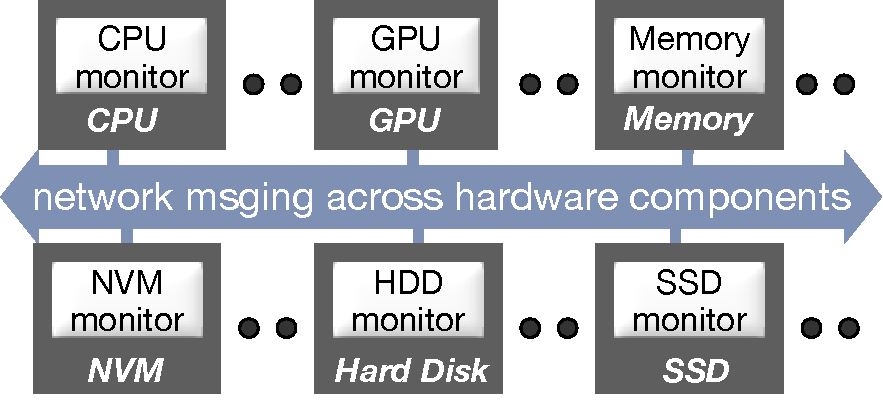
\includegraphics[width=2.6in]{lego/Figures/lego-arch.pdf}}
\caption[Splitkernel Architecture.]{Splitkernel Architecture.}
\label{fig-splitkernel}
\end{center}
\end{subfigure}
\caption[Operating System Architecture.]{Operating System Architecture.}
\end{figure*}
}

We built {\em \sys}, a hardware-based disaggregated memory system (Figure~\ref{fig-arch}).
%focusing on the hardware-based virtual memory system and network stack.
\sys\ includes a \CN-side user-space library called {\em \syslib}
and a new hardware-based \MN\ device called {\em \sysboard}.
Multiple application processes running on different \CN{}s could allocate memory from the same \sysboard, with each process having its own {\em remote virtual memory address space}.
Applications access their remote memory space using APIs that \sys\ provides (\eg, \alloc, \sysread, \syswrite, \syslock), and the accesses are in byte granularity.
For each API, \sys\ provides a synchronous version and an asynchronous version, with the former following sequential consistency and the latter following release consistency.

A \sysboard\ consists of three main components: 1) a hardware chip that integrates a thin network stack and a virtual memory system to handle data requests (the {\em fast path}), 2) an ARM processor that runs software to handle metadata requests and background tasks (the {\em slow path}), and 3) an FPGA that hosts application computation offloading (the {\em extend path}).

In building \sys, we explore new requirements, challenges, and benefits of \md.
Specifically, we answer three important research questions.

First, \textbf{how does the design and implementation of a
dedicated hardware \MN\ differ from server and programmable NIC
designs?}
%To protect the accesses from different applications to the memory in an \MN\ and to make such accesses flexible, 
%we should use a virtual memory system to check and map virtual memory addresses to physical addresses.
Current \md\ solutions rely on a host server (its OS and MMU) to provide a virtual memory system so that accesses to the memory are protected and flexible. 
Using a whole server just for the virtual memory system is overkill and unnecessarily adds monetary and energy costs to \md. %consumes too much power.
Another possibility is to use a low-power processor (\eg, ARM) in a SmartNIC to run the virtual memory system~\cite{iPipe}. 
However, doing so has high performance impact mainly because the virtual memory system is on a separate chip from the NIC.
%However, doing so has performance overhead, both because the virtual memory system is on a separate chip from the NIC
%and because the virtual memory system is not designed for \md.
%To date, there has been no attempt
%\yizhou{I think here we should emphasize that: MNs emulated using host server has cost and power waste while the SmartNIC-based ones have perf issue. In all, there is no ideal solution for building real server-less MNs. Hence we took a ...}
Overall, server-based approaches have cost overheads while SmartNIC solutions have performance overheads.
We took a clean-slate approach by building a hardware-based virtual memory system that is integrated with a customized hardware network stack, 
both of which are designed specifically for handling virtual memory requests sent over the network.

Second, \textbf{how can a low-cost \MN\ host TBs of memory and support thousands of concurrent application processes?}
Different from traditional (local) memory, an \MN\ is intended to be shared by many applications running at different \CN{}s,
and the more applications it can support, the more efficiently its memory can be utilized.
Thus, we aim to have each \MN\ host TBs of memory for thousands of concurrent applications processes.
However, a hardware design is constrained by the limited resources in a hardware chip such as on-chip memory.
Compared to traditional software-based virtual memory systems, 
how can an \MN\ use orders of magnitude less resources while achieving orders of magnitude higher scalability?
%which raises the problem of how to manage the scalability we target in hardware.
%is especially accute in an \hdm\ because of its low cost requirements.
Current solutions like RDMA NICs swap metadata between NIC's on-chip memory and host server memory,
which comes with performance overhead (4\x\ compared with when metadata is in the NIC memory~\cite{Pythia}).
%RDMA improves scalability by adding more hardware resources to cache more metadata/states), which comes with increasing monetary and energy costs.

Our clean-slate approach is to carefully examine each virtual-memory and networking task 
and to redesign them to \textbf{1)} eliminate states and metadata whenever possible (\eg, by eliminating the RDMA "Memory-Region" concept),
\textbf{2)} move complex but non-performance-critical states, metadata, and tasks to the software slow path,
\textbf{3)} shift functionalities to the \CN\ (\syslib) to reduce \MN's complexity 
(\eg, our reliable network transport runs at \syslib, and \MN\ is ``transport-less''; we achieve reliability by ordering and retrying at the memory request level instead of the packet level),
and \textbf{4)} design bounded-size, inherently scalable data structures (we propose a new page table design that lets all processes share one global page table whose size is determined by the physical memory size).
%For the remaining functionalities that still need caching, we redesign them to guarantee good cache-miss performance.
As a result, each \MN\ (\sysboard) could support TBs of memory and thousands of application processes with only 1.5\MB\ on-chip memory.
%\yizhou{On top of network scalability, I think its also worth explaining how we are able to support TBs of memory. Because this reminds me of O(1) memory issues. With TBs of memory, the memory related metadata and OPs increased as well. Our pros: our fast path use huge page + hashtable-based pgtable, bounded latency. Our cons: our buddy allocator running in ARM is still prone to this huge memory issue.}
%For certain functionalities, we avoid states and metadata alltogether by re-designing the functionalities.
%For functionalities that could be and move the ones that can be moved to the \CN\ side.
%and not relying on cache for good performance.

Third, \textbf{how to minimize tail latency in a \md\ system}?
%\textbf{is it possible to minimize tail latency by processing all read/write requests deterministically?} 
Tail latency is important in data centers especially for workloads that have large fanouts (\eg, Spark jobs).
Although much effort has focused on improving the network and core scheduling for low tail latency~\cite{nanoPU,Shenango,Shinjuku,ZygOS,RPCValet},
the memory system has largely been overlooked.
However, the (remote) memory system is what contributes to extreme long tails in a \md\ system.
For example, RDMA's round-trip latency is around 1--2\mus\ in the common case,
but its tail could be as long as 16.8\ms. % (when there is a page fault).
%The main reason for RDMA's various tails is its reliance on the host virtual memory system, which is not designed for \md\ or for low tail latency.

We reexamine traditional memory system
%from the tail latency and perspectives 
and propose a set of novel mechanisms to bound \sys's tail latency.
Our core idea is to include {\em all} the functionalities that are needed to fulfill all types of data requests in one hardware pipeline
and to make this hardware pipeline {\em performance deterministic}.
This pipeline takes one incoming data unit every cycle (\ie, no pipeline stalls) and completes every request in a fixed number of cycles.
Two major technical hurdles in achieving this performance are to perform page table lookups and to handle page faults in a bounded, short time period.  
For the former, we propose a new {\em overflow-free} hash-based page table that bounds all page table lookups to {\em at most one DRAM access} (instead of the long page table walk in a traditional CPU architecture).
Our novel idea is to avoid overflows at the virtual memory address allocation time, by retrying the allocation until a non-overflow virtual memory address range is found.
For the latter, we propose a new mechanism to handle page faults in hardware with bounded cycles (instead of the costly process of interrupting and handling page faults in OS).

%These mechanisms include 1) handling page faults in hardware,
%2) d
%RDMA’s way is to pre-reserve memory and to use large on-device cache. But cache can’t always work, and reserving memory results in inefficient memory utilization.
%Our solution is to allocate physical memory on-demand and to make the cache miss path fast by handling page faults in hardware and by designing a new hash-based page table. We also carefully designed our hardware pipeline to have deterministic, bounded latency.

\section{Main Artifacts and Key Results}

{
\begin{figure*}[th]
\begin{center}
\centerline{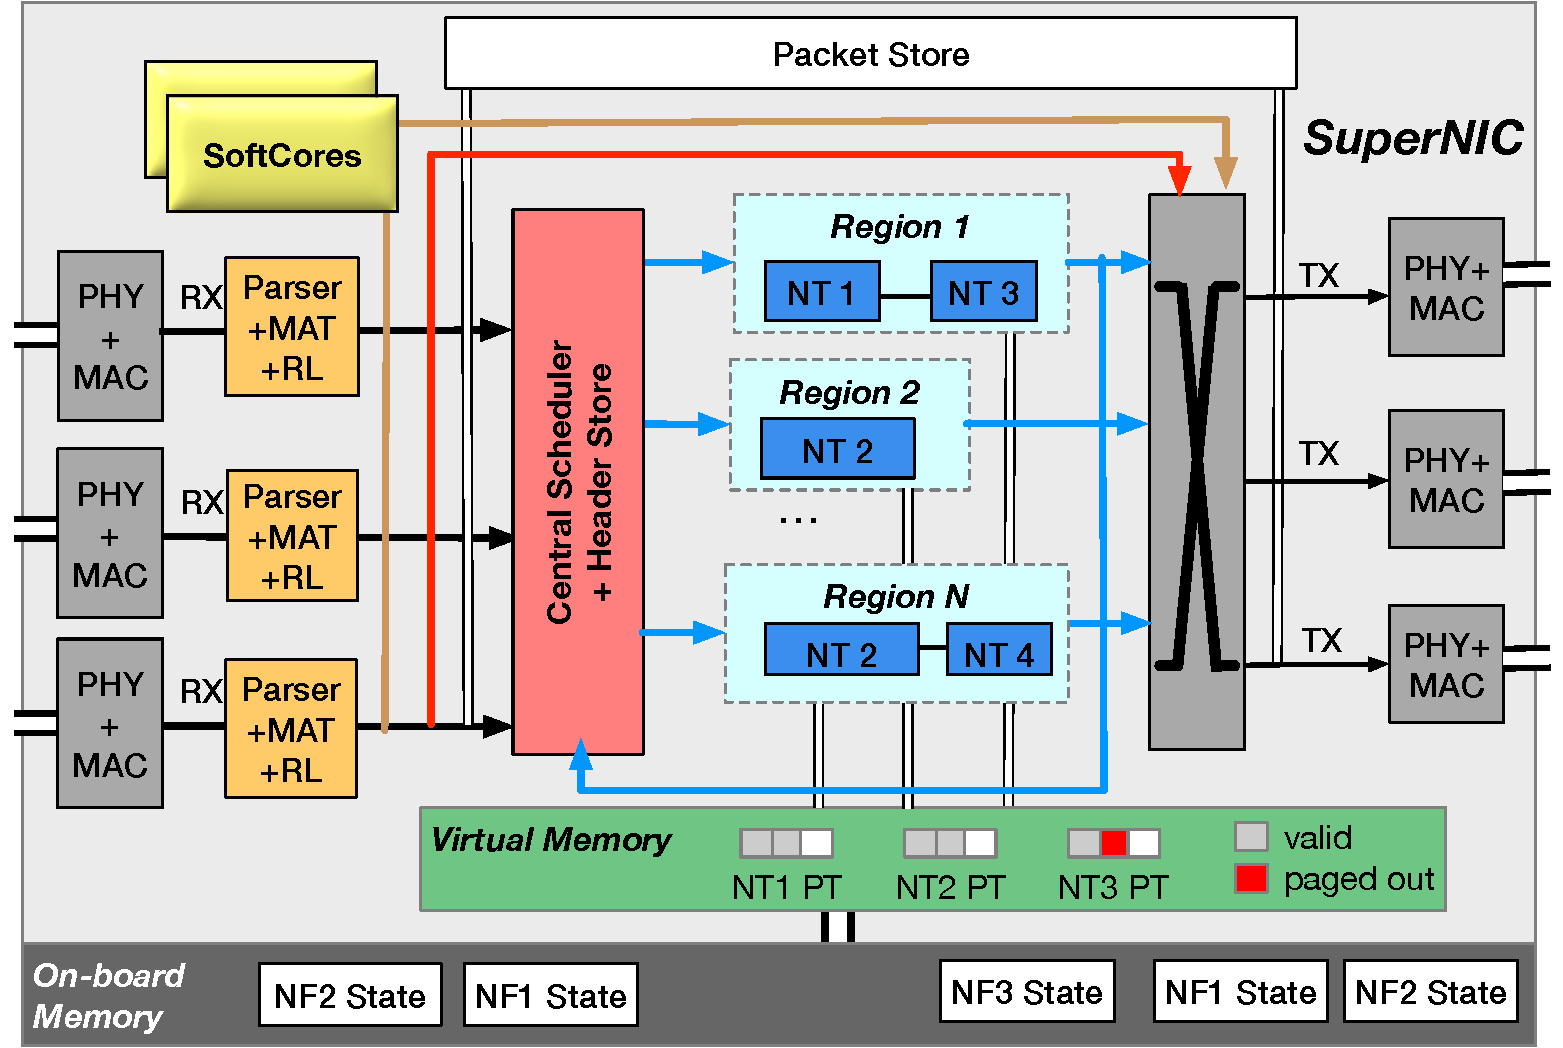
\includegraphics[width=\textwidth]{snic/Figures/board.pdf}}
\mycaption{fig-snic-board}{\snic\ On-Board Design.}
{
RL: Rate Limiter. PT: Page Table
}
\end{center}
\end{figure*}
}
{
\begin{figure*}[th]
\begin{center}
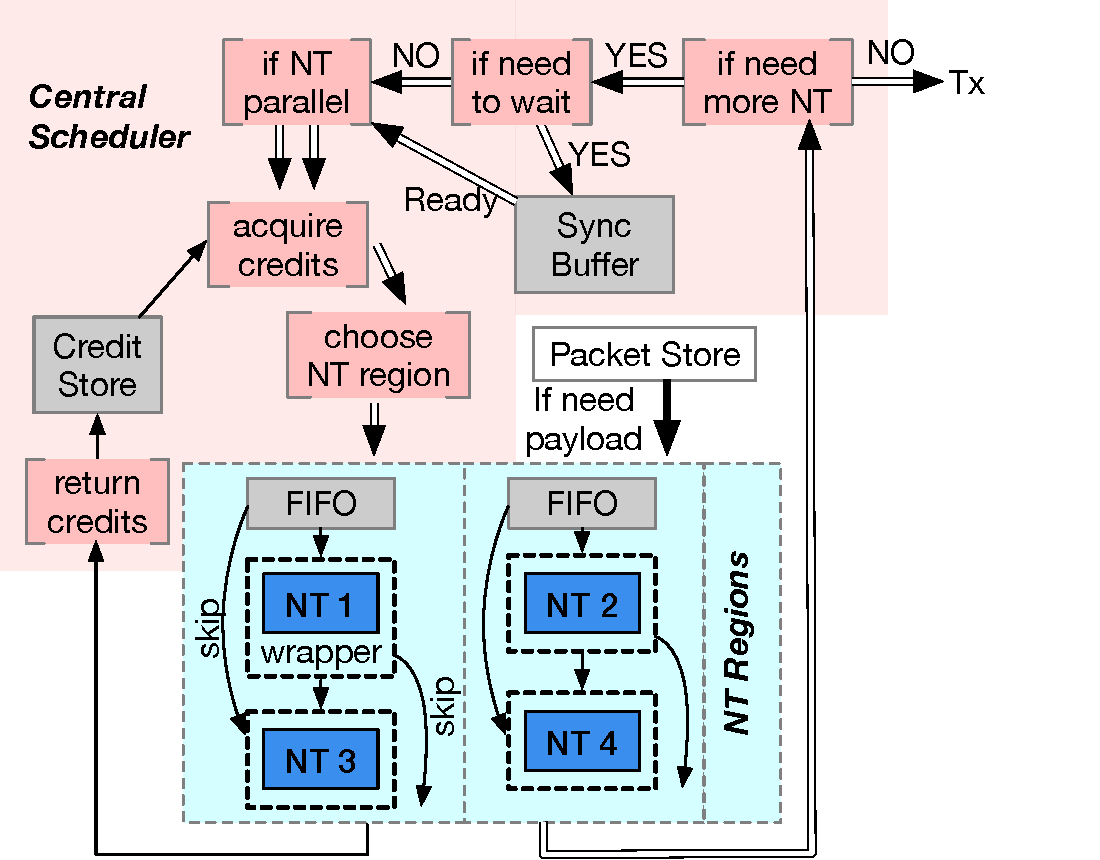
\includegraphics[width=0.9\textwidth]{snic/Figures/scheduler.pdf}
\mycaption{fig-sched}{\snic\ Packet Scheduler and \nt\ Region Design.}
{
Double arrows, single arrows, and thick arrows represent packet headers, credits, and packet payload.
}
\end{center}
\end{figure*}
}

We prototyped \sysboard\ with a Xilinx MPSoC FPGA board~\cite{ZCU106} and implemented \syslib\ as a user-space library on Linux servers. 
Figure~\ref{fig-coremem} illustrates the overall board-level design.
We built three applications using \sys:
a FaaS-style image compression utility, a radix-tree index, and a key-value store.
%We prototyped \sys's memory device with FPGA (\sysboard).
%\sys\ achieves high throughput (100\Gbps\ with FPGA prototype), low (tail) latency (XXX\mus\ end-to-end MTU round trip latency), 
%low cost (XXX\x\ energy saving), %and great extendibility,
%and \sys\ scales well with XXX. %eliminates {\em all} scalability bottlenecks in both its memory and network systems.
Our FPGA \sys\ prototype achieves 100\Gbps\ throughput and an end-to-end latency of 2.5\mus\ at median and 3.2\mus\ at 99-percentile.
We compared \sys\ with native RDMA, two RDMA-based disaggregated/remote memory systems~\cite{Tsai20-ATC,Kalia14-RDMAKV}, 
a software emulation of hardware-based disaggregated memory LegoOS~\cite{Shan18-OSDI},
%an FPGA-based RDMA implementation~\cite{StRoM}, 
and a software-based SmartNIC BlueField~\cite{BlueField}.
\sys\ scales much better and has orders of magnitude lower tail latency than RDMA, 
while achieving similar throughput and median latency as RDMA (even with the slower FPGA frequency in our prototype).
\sys\ has 1.1\x\ to 3.4\x\ energy saving compared to CPU-based and SmartNIC-based disaggregated memory systems 
and is 2.7\x\ faster than software-based SmartNIC solutions. 
%We will make \sys\ publicly available upon this paper's publication.


Overall, this paper makes the following contributions.

\begin{itemize}

\item The first publicly described hardware-based disaggregated memory system and an FPGA prototype.

\item A demonstration of how to co-design system software (a full virtual memory system), hardware architecture (memory management unit), and networking stack (a customized reliable network).

\item A demonstration of how to co-design the compute and the memory sides in a disaggregated system.

\item A demonstration of how to separate data and control plane in a virtual memory system for disaggregated memory.

\item Three applications built with real disaggregated memory, with some offloading their computation to memory devices.
%\item Hardware-based distributed operation support such as migration and replication.

% and a set of extended virtual memory APIs. 
%\item Demonstration of how real systems could use and benefit from disaggregated memory services.

%\item Two hardware-based high-level distributed memory services.
%\item Demonstration of two deployment models of disaggregated memory hardware.

\end{itemize}



%\subsection*{Why ASPLOS}
%\label{sec:why-asplos}
\section{Why ASPLOS}
This paper demonstrates how to implement a core OS functionality, the virtual memory system, in hardware in a non-conventional way.
We also demonstrate how to co-design hardware and software.
Thus, this paper fits well with the scope of ASPLOS in
architecture and system.
 
\pagebreak
%\bibliographystyle{plain}
%\bibliography{all-defs,all,personal,all-confs,local,paper}


%\end{document}




  %%%%%%%%%%%%%%%%%%%%%%%%5
%\clearpage
%\pagestyle{empty}
%\input{department}
\clearpage






%\setstretch{1}
%\bibliography{ws1,ws2,asplos,fpga,full,hot-chips,immd4,microchip,other,BuildingStuff}

\setstretch{0.8}
\titlespacing*{\section}{0em}{1ex}{1ex}
\begin{small}

%\bibliographystyle{ieeetr}
\begin{spacing}{0.3}
\bibliographystyle{abbrv}
%\bibliographystyle{mbt_dj}
\bibliography{all-defs,all,personal,all-confs,local,paper}
\end{spacing}
\end{small}

%\clearpage
%\input{bio}
%\clearpage
%\input{budget}
%\clearpage
%\input{facilities}

\end{document}





\clearpage

\appendix

\section{Appendix}

\subsection{FPGA Resource Utilization}

The following table shows the FPGA resources used by \snic{} shell.
Most of the resources are left for running \nt{}s.

\begin{center}
\scriptsize
\begin{tabular}{ p{0.6in} | p{0.2in} |p{0.27in} }
 & \textbf{Logic} & \textbf{Memory} \\
\textbf{Module} & \textbf{(LUT)} & \textbf{(BRAM)} \\
\hline
\hline
%Firewall     & 2.8\% & 0.5\% \\
%AES-256       & 0.4\% & 0 \\
%Transport    & 1.3\% & 0.42\% \\
%\hline
%\hline
\snic{} Core & 4.36\%   & 4.74\% \\
Packet Store & 0.91\%   & 9.17\% \\
PHY+MAC      & 0.72\%   & 0.35\% \\
DDR4Controller         & 1.57\%   & 0.29\% \\
MicroBlaze   & 0.25\%   & 1.81\% \\
Misc         & 1.52\%   & 0.75\% \\
%\textbf{Total (w/o \nt{})}        & \textbf{9.33\%}   & \textbf{17.11\%} \\
\hline
\textbf{Total}        & \textbf{9.33\%}   & \textbf{17.11\%} \\
\end{tabular}
\end{center}



\subsection{Cost Calculation}
We explain the different deployment models and the cost calculation formulas behind our CapEx comparisons.
We limit our scope to rack-scale as the higher-level network hierarchies
are orthogonal to the resource pool deployment models.
We calculate that, to deploy a certain number of endpoints, what's the
network cost (i.e., the network interface card, cable, and switch port costs).

We compare the following models:
1) Non-disaggregation model, or the traditional model, termed \texttt{traditional}.
2) Disaggregation model, in which we insert the network pool between endpoints and the ToR switch (Figure~\ref{fig-topology} (a)), termed \texttt{ring}.
3) Disaggregattion model, in which we connect the pool of network devices directly to the ToR switch (Figure~\ref{fig-topology} (b)), termed \texttt{direct}.
For both disaggregation models, we further compare two type of devices: sNIC which has auto-scaling capability and multi-host NIC which can only provision for max resource usage. With runtime dynamic scaling and load balancing features, sNICs can provision for less than the max required resource , the specific ratio is calculated by comparing a particular workload's the sum-of-peak versus the peak-of-sum.

In all, we have the following models under comparison:
\texttt{traditionl, sNIC-direct, sNIC-ring, mhnic-direct, mhnic-ring}.

We now detail the cost calculations.
In the traditional non-disaggregation model,
each endpoint has a full-fledged NIC and a normal high-speed cable for connection to the ToR switch.
In both disaggregation models, since most network tasks are offloaded to the network resource pool, each endpoint can uses a down-scaled NIC.
Furthermore, the last hop link layer between endpoints and the network resource pool is reliable, we can leverage down-scaled, cheaper and less reliable physical cable~\cite{RAIL-NSDI}.

We use the following parameters in our calculation:
\begin{itemize}
\item Deploy \texttt{N} devices.
\item Each switch port has a cost of \texttt{costSwitchPort}
\item A full-fledged NIC's cost is \texttt{costNIC}. A down-scaled NIC cost is \texttt{costDSNIC}.
\item A normal high-speed cable cost is \texttt{costCable}.
A down-scaled less reliable physical cable cost is \texttt{costDSCable}.
\item A consolidation ratio \texttt{consolidRatio} determines how many endpoints are sharing one network resource pool device. We can calculate the number of network pool devices by \texttt{M = N / consolidRatio}.
\item For a network device, only a certain portion is dedicated to running network task, other parts are used as shell. We define the cost ratio used by network task to be \texttt{NTCostRatio}.
\item The peak-of-sum versus the sum-of-peak yields the auto-scaling potentials. A multi-host NIC (mhnic) provisions for the sum-of-peak while an sNIC provisions for the peak-of-sum. We call this ratio \texttt{capExConsolidRatio}.
\item The multi-host NIC's cost can be calculated as \texttt{costMHNIC = costNIC * N}.
\item The sNIC's cost can be calculated as \texttt{costsNIC = costMHNIC * capExRatio}, in which \texttt{capExRatio = (1 - NTCostRatio) + NTCostRatio * capExConsolidRatio}.
\end{itemize}

We now define each model's cost.

The traditional deployment model's cost is straightforward, it includes NIC, cable and switch ports:
\begin{gather}
N * (costNIC + costCable + costSwitchPort)
\end{gather}

The disaggregation models' cost has more moving parts than the traditional. It includes the down-scaled NICs and cables, network pool devices, the cables to the ToR switch, and switch ports.

The first disaggregation model (Figure~\ref{fig-topology} (a)) can be calculated as follows (for both \texttt{sNIC-ring, mhnic-ring}). 
\begin{align}
N * (costDSNIC + costDSCable) + \\
M * (costsNIC + costCable + costSwitchPort)
\end{align}

The second disaggregation model (Figure~\ref{fig-topology} (b)) can be calculated as follows (for both \texttt{sNIC-direct, mhnic-direct}).
\begin{align}
N * (costDSNIC + costCable + costSwitchPort) + \\
M * (costsNIC + costCable + costSwitchPort)
\end{align}

This tables shows the real-world numbers we use.

\begin{center}
\scriptsize
\begin{tabular}{|l|l|l|} 
 \hline
 Parameters & Value & Note \\
 \hline\hline
 costSwitchPort & \$250 & FS 100Gbps switch~\cite{fs-64port-switch} \\
 costNIC & \$500 & Mellanox Connect-X5 \\
 costCable & \$100 & FS DAC 100Gbps cable \\
 costDSNIC & costNIC * 0.2 & Numbers from our prototpe \\
 costDSCable & costCable * 0.6 & ~\cite{RAIL-NSDI} \\
 consolidRatio & 4 & Current model\\
 NTCostRatio & 0.9 & Numbers from our prototype \\
 capExConslidRatio & 0.23 & Facebook Hadoop trace~\cite{facebook-sigcomm15} \\
 \hline
\end{tabular}
\end{center}

%\subsection{Extended Evaluation Results}

{
\begin{figure*}[th]
\begin{minipage}{\figWidthSix}
\begin{center}
\centerline{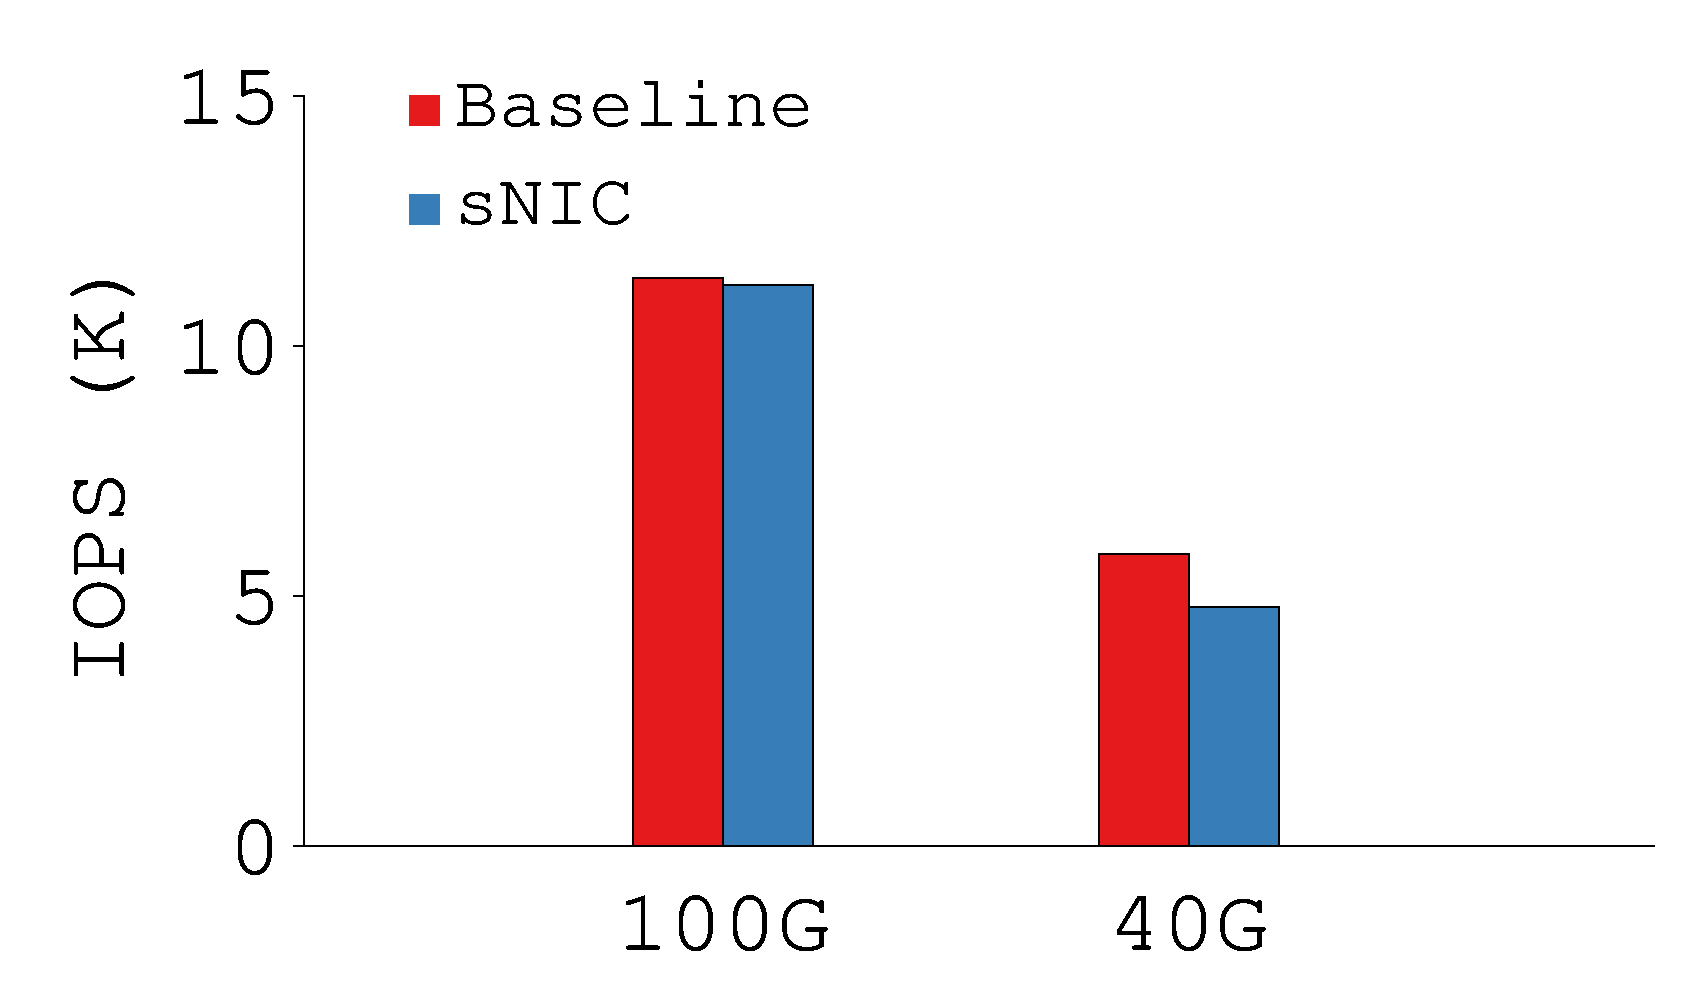
\includegraphics[width=\columnwidth]{Figures/g_plot_conslid_perf.pdf}}
\vspace{-0.1in}
\mycaption{fig-kv-consolid}{Consolidation Performance w/ FB Key-Value.}
{
}
\end{center}
\end{minipage}
\begin{minipage}{\figWidthSix}
\begin{center}
\centerline{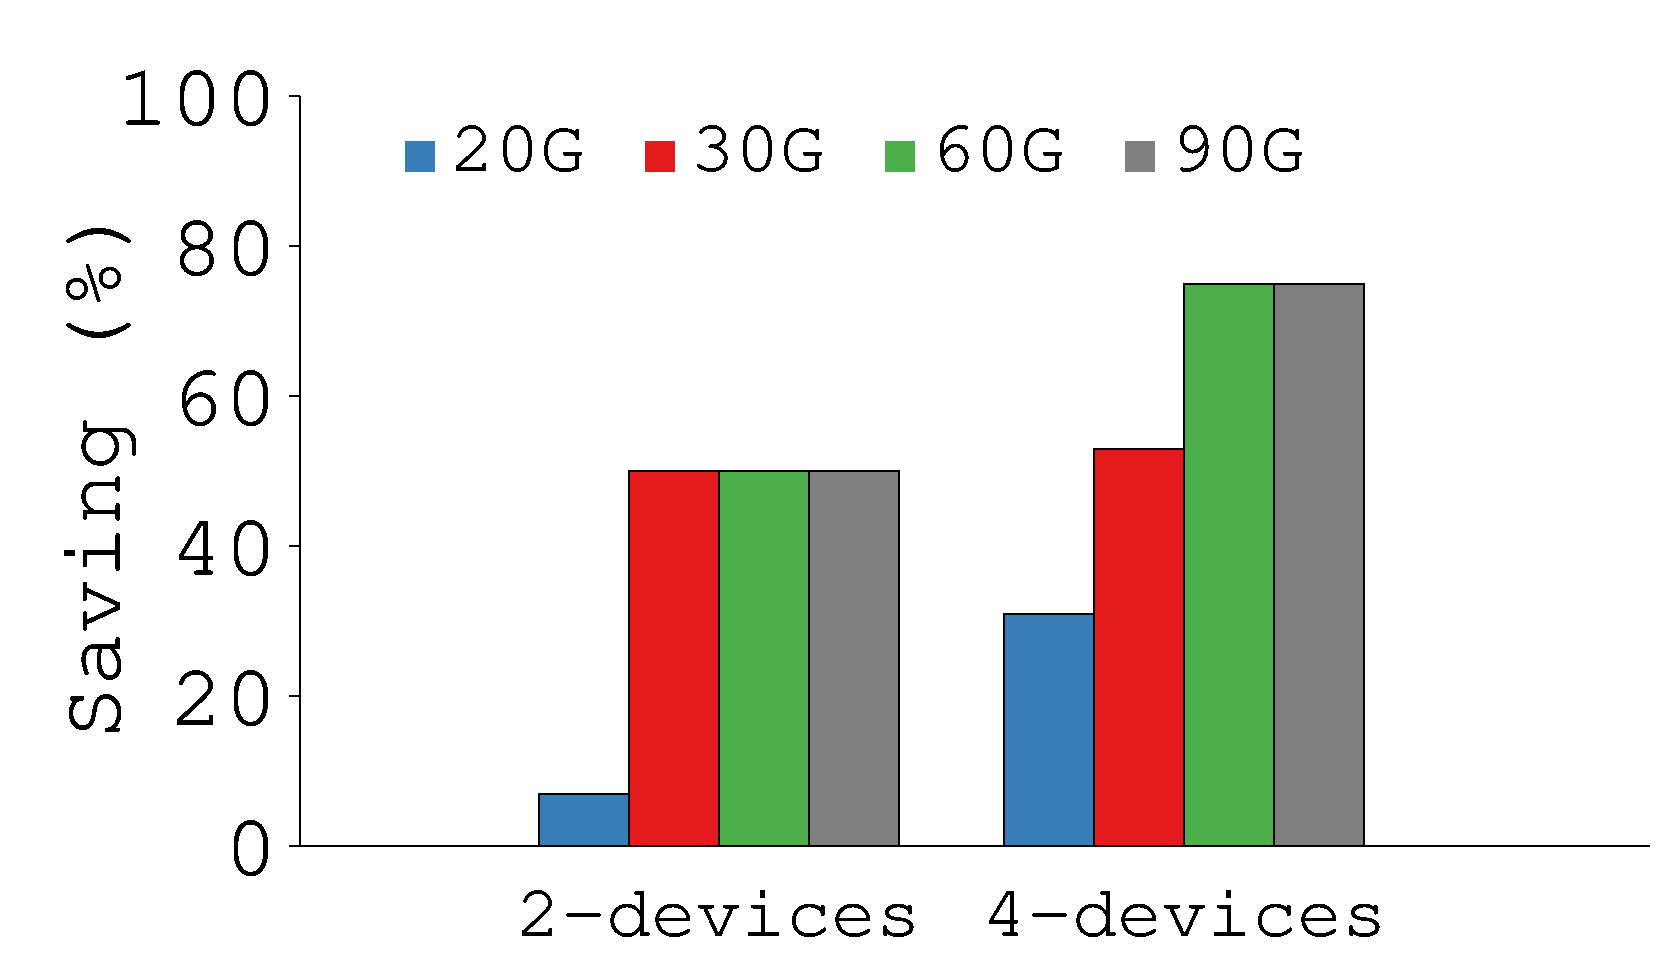
\includegraphics[width=\columnwidth]{Figures/g_plot_conslid_cost.pdf}}
\vspace{-0.1in}
\mycaption{fig-kv-cost}{Consolidation Resource Usage w/ FB KV.}
{
}
\end{center}
\end{minipage}
\vspace{-0.1in}
\end{figure*}
}
\subsection{End-to-End Application Performance and Cost with Consolidation}

To evaluate the benefit and tradeoff of consolidation, we deploy a testbed with four sender and four receiving servers with four setups:
each endhost connects to a ToR switch with 100\Gbps\ or 40\Gbps\ link (baseline, no consolidation), and four endhosts connect to an \snic, each with 100\Gbps\ or 40\Gbps\ link, and the \snic\ connects to the ToR switch with a 100\Gbps\ or 40\Gbps\ link (\snic\ consolidation).
%, and 3) four endhosts connect to an emulated multi-host NIC, each with a 25\Gbps\ link (\S\ref{sec:related}), and the multi-host NIC connects to the ToR switch with a 100\Gbps\ link. %(multi-host NIC, statically partitioned link bandwidth).
For both settings, we execute two \nt{}s, firewall and NAT, in FPGA. 
For the baseline, each endhost has its own set of \nt{}s, while %the multi-host NIC uses one set of \nt{}s in total and 
\snic\ autoscales \nt{}s as described in \S\ref{sec:policy}.
On each server, we generate traffic to follow inter-arrival and size distribution reported in the Facebook 2012 key-value store trace~\cite{Atikoglu12-SIGMETRICS}.
%the Hadoop load distribution reported in the 2015 Facebook workloads~\cite{facebook-sigcomm15}.
%Since there is no reported inter-arrival time for these workloads, we use the inter-arrival time reported by the 2012 Facebook workloads~\cite{Atikoglu12-SIGMETRICS}.
%We measure the application throughput (IOPS) every 10\ms\ time unit to evaluate the throughput changes over time.

Figure~\ref{fig-kv-consolid} reports the throughput comparison of \snic\ and the baseline.
%average IOPS and 95-percentile IOPS across all time units for the three settings. 
\snic\ only adds 1.3\% performance overhead to the baseline under 100\Gbps\ network and 18\% overhead under 40\Gbps\ network. 
We further analyze the workload and found its median and 95-percentile loads to be 24\Gbps\ and 32\Gbps.
With four senders/receivers, the aggregated load is mostly under 100\Gbps\ but often exceeds 40\Gbps.
Note that a multi-host NIC would not be able to achieve \snic's performance, as it subdivides the 100\Gbps\ or 40\Gbps\ into four 25\Gbps\ or 10\Gbps\ sub-links, which would result in each endhost exceeding its sub-link capacity.


We then calculate the amount of FPGA used for running the \nt{}s multiplied by the duration they are used for, to capture the run-time resource consumption with \snic's autoscaling mechanism. The baseline has one set of \nt{}s per endhost for the whole duration.
Figure~\ref{fig-kv-cost} shows this comparison when consolidating two and four endhosts to an \snic\ and using \nt{}s of different performance metrics.
For a slower \nt{} (\eg, one that can only sustain 20\Gbps\ max load), the \snic\ auto-scales more instances of it, resulting in less cost saving.
Our implementation of firewall \nt{} reaches 100\Gbps, while the AES \nt\ is 30\Gbps, resulting in a 64\% cost saving when deploying both of them.



%On the other hand, multi-host NIC incurs higher performance overhead, especially for the tail.
%Whenever any endhost exceeds 25\Gbps\ load, multi-host NIC will have a bottleneck link.
%On the other hand, \snic\ can sustain the peak of aggregated traffic, which is mostly under 100\Gbps, demonstrating the benefit of run-time, dynamic consolidation.

\if 0
\subsubsection{Distributed \snic{}}
To run an \nt\ at a remote \snic,
an \snic{}'s SoftCore first sends a control message to the remote \snic{} to launch the \nt{} and then installs forwarding rules to its parser. This process takes 2.3\mus\ in our testbed.
Afterwards, packets are forwarded to the remote \snic. We observe an addition of 1.3\mus\ latency when packets go through the remote \snic.
\fi

\end{document}